\documentclass[a4paper, 11pt, oneside]{report}

\usepackage{preamble}

\begin{document}

\begin{titlepage}

  \centering

  {\fontsize{50}{60}\textbf{Análisis Real}}

  \vspace{4\baselineskip}

  {\fontsize{15}{18}
  
  Universidad de Málaga

  \vspace{0.5\baselineskip}

  Grado en Matemáticas

  \vspace{0.5\baselineskip} % por algún motivo, tras la primera línea hay más espacio en blanco

  Curso 2024-2025}

  \vspace{4\baselineskip}

  \begin{figure}[H]
    \centering
    \begin{subfigure}[b]{0.49\textwidth}
      \centering
      \fbox{\includegraphics{./plot27/main.pdf}}
    \end{subfigure}
    \begin{subfigure}[b]{0.49\textwidth}
      \centering
      \fbox{\includegraphics{./plot28/main.pdf}}
    \end{subfigure}
  \end{figure}
  
  \begin{figure}[H]
    \centering
    \begin{subfigure}[b]{0.49\textwidth}
      \centering
      \fbox{\includegraphics{./plot29/main.pdf}}
    \end{subfigure}
    \begin{subfigure}[b]{0.49\textwidth}
      \centering
      \fbox{\includegraphics{./plot30/main.pdf}}
    \end{subfigure}
  \end{figure}

\end{titlepage}

\tableofcontents
\thispagestyle{empty}

\chapter{Espacios \texorpdfstring{\textit{L\textsuperscript{p}}}{\textit{Lp}}}

\section{Funciones convexas}

Puesto que las funciones convexas ya se estudiaron en la asignatura \emph{Análisis Matemático II}, las demostraciones de algunos resultados van a ser omitidas.

\begin{definition}
  Sea $I \subset \R$ un intervalo y sea $\varphi \colon I \to \R$. Decimos que $\varphi$ es \emph{convexa en $I$} (o simplemente \emph{convexa}) si para todos $x,y\in I$ con $x<y$ y todo $\lambda \in (0,1)$ se tiene que
  \[\varphi(\lambda x + (1-\lambda)y) \leq \lambda \varphi(x)+(1-\lambda) \varphi(y).\]
\end{definition}

Equivalentemente, una función $\varphi$ es convexa en $I$ si para todos $a,b,x \in I$ con $a<x<b$ se tiene que 
\[\frac{\varphi(x)-\varphi(a)}{x-a} \leq \frac{\varphi(b)-\varphi(a)}{b-a}.\]

Gráficamente, $\varphi$ es convexa si para $a,b \in I$ cualesquiera con $a<b$, la gráfica de $\varphi$ en $[a,b]$ queda por debajo del segmento que une $(a,f(a))$ con $(b,f(b))$.

\begin{figure}[H]
  \centering
  \includegraphics{./plot1/main.pdf}
  \caption{Interpretación gráfica de la convexidad.}
\end{figure}

\begin{proposition}
  Sea $I \subset \R$ un intervalo. Si $\varphi \colon I \to \R$ es convexa en $I$ y $x_0 \in \mathring{I}$, entonces existen $\varphi'_-(x_0)$ y $\varphi'_+(x_0)$. Además, $\varphi'_-(x_0) \leq \varphi'_+(x_0)$.
\end{proposition}

\begin{corollary}
  Si $I \subset \R$ es un intervalo y $\varphi \colon I \to \R$ es convexa en $I$, entonces $\varphi$ es continua en $\mathring{I}$.
\end{corollary}

\begin{definition}
  Sea $I \subset \R$ un intervalo abierto, sea $\varphi \colon I \to \R$ una función convexa en $I$ y sea $x_0 \in I$. Llamamos \emph{recta soporte de $\varphi$ en $x_0$} a cualquier recta que pase por $(x_0,\varphi(x_0))$ y cuya pendiente $m$ verifique $\varphi'_-(x_0) \leq m \leq \varphi'_+(x_0)$.
\end{definition}

La ecuación de cualquier recta soporte de $\varphi$ en $x_0$ es $y = \varphi(x_0)+m(x-x_0)$, donde $\varphi'_-(x_0) \leq m \leq \varphi'_+(x_0)$.

\begin{proposition}
  Sea $I \subset \R$ un intervalo abierto y sea $\varphi \colon I \to \R$ una función convexa en $I$. Sea $x_0 \in I$ y sea $y = \varphi(x_0)+m(x-x_0)$ una recta soporte de $\varphi$ en $x_0$. Entonces para todo $x \in I$ se verifica
  \[\varphi(x) \geq \varphi(x_0)+m(x-x_0),\]
  es decir, las rectas soporte de $\varphi$ en $x_0$ quedan por debajo de la gráfica de $\varphi$.
\end{proposition}

\begin{proof}
  Sea $x \in I$. Si $x = x_0$, se da la igualdad. Si $x < x_0$, entonces
  \[\frac{\varphi(x)-\varphi(x_0)}{x-x_0} \leq \varphi'_-(x_0) \leq m,\]
  de donde se deduce que
  \[\varphi(x) \geq \varphi(x_0) + m(x-x_0),\]
  teniendo en cuenta que $x-x_0 < 0$. Si $x>x_0$, se procede de forma totalmente análoga.
\end{proof}

\begin{example}
  Sea $\varphi \colon \R \to \R$, $\varphi(x)=|x|$. Como $\varphi'_+(0)=1$ y $\varphi'_-(0)=-1$, las rectas soporte de $\varphi$ en $0$ son las de ecuación $y = mx$ con $-1 \leq m \leq 1$.

  \begin{figure}[H]
    \centering
    \includegraphics{./plot2/main.pdf}
    \caption{Rectas soporte de la función valor absoluto.}
  \end{figure}

\end{example}

\section{Cuatro desigualdades importantes}

\begin{theorem}[Desigualdad de Jensen]\label{teo:1.2.1}
  Sea $(X,\mathcal{M},\mu)$ un espacio de probabilidad, sea $I \subset \R$ un intervalo abierto y sea $f \colon X \to I$ medible y con $\int_X |f| \, d\mu < \infty$. Si $\varphi \colon I \to \R$ es convexa en $I$, entonces
  \[\varphi\left(\int_X f \, d\mu\right) \leq \int_X \varphi \circ f \, d\mu.\]
\end{theorem}

\begin{proof}
  Obsérvese que $\varphi \circ f$ está bien definida porque $f(X) \subset I$, y es medible porque $f$ es medible y $\varphi$ es continua. Sea $x_0 = \int_X f \, d\mu$ y veamos que $x_0 \in I$. Suponemos que $I = (a,b)$ con $a,b \in \R$ (si fuese $a = -\infty$ o $b = \infty$ se razona análogamente). Sabemos que $a < f(x) < b$ para todo $x \in X$, así que
  \[\int_X a \, d\mu < \int_X f \, d\mu = x_0 < \int_X b \, d\mu.\]
  Pero $\int_X a \, d\mu = a\mu(X) = a$ y $\int_X b \, d\mu = b\mu(X) = b$, luego $a < x_0 < b$.

  Ya podemos empezar a probar la desigualdad del enunciado. Sea $y = \varphi(x_0)+m(x-x_0)$ una recta soporte de $\varphi$ en $x_0$. Por la proposición anterior, para todo $t \in I$ se verifica 
  \[\varphi(t)\geq \varphi(x_0)+m(t-x_0).\]
  En particular, si $x \in X$,
  \[\varphi(f(x))\geq \varphi(x_0)+m(f(x)-x_0).\]
  Nótese que la función dada por $x \mapsto \varphi(x_0)+m(f(x)-x_0)$, $x \in X$, es medible e integrable, ya que $f$ lo es integrable y $\mu(X) = 1$. En consecuencia, por la desigualdad anterior, $\varphi \circ f$ es integrable en sentido amplio. Además, también por dicha desigualdad,
  \[
  \begin{aligned}[t]
    \int_X \varphi \circ f (x)\, d\mu(x) &\geq \int_X \left(\varphi(x_0)+m(f(x)-x_0)\right) \, d\mu(x) \\ 
    &= \int_X \varphi(x_0)\, d\mu(x)+m\int_X f(x) \, d\mu(x)-m\int_X x_0 \, d\mu(x) \\
    &= \varphi(x_0)+mx_0 - mx_0 \\
    &= \varphi(x_0),
  \end{aligned}\]
  que es lo que queríamos probar.
\end{proof}

Se podría permitir que la función $f$ del teorema anterior tomase valores en $\overline{\R}$, pero el hecho de que sea $\int_X |f| \, d\mu < \infty$ implica que $|f| < \infty$ en casi todo punto de $X$, de ahí que se considere que toma valores finitos.

\begin{example}
  Sea $(X,\mathcal{M},\mu)$ un espacio de probabilidad y sea $f \colon X \to \R$ una función medible y con $\int_X |f| \, d\mu < \infty$.
  \begin{enumerate}
    \item La función $\varphi(x)=e^x$ es convexa en $\R$, así que la \hyperref[teo:1.2.1]{\color{c1}desigualdad de Jensen} afirma que
    \[e^{\int_X f \, d\mu} \leq \int_X e^f \, d\mu.\]
    \item La función $\varphi(x)=x^2$ es convexa en $\R$, así que la \hyperref[teo:1.2.1]{\color{c1}desigualdad de Jensen} afirma que
    \[\left(\int_X f \, d\mu\right)^2 \leq \int_X f^2 \, d\mu.\]
    \item Si $p \geq 1$, la función $\varphi(x)=x^p$ es convexa en $(0,\infty)$, y si $f(x)>0$ para todo $x \in X$, por la \hyperref[teo:1.2.1]{\color{c1}desigualdad de Jensen},
    \[\left(\int_X f \, d\mu\right)^p \leq \int_X f^p \, d\mu.\]
    \item Si $f(x)>0$ para todo $x \in X$ y $\int_X |\log f| \, d\mu < \infty$, por el primer apartado,
    \[e^{\int_X \log f \, \mu} \leq \int_X e^{\log f} \, d\mu = \int_X f \, d\mu.\]
    Tomando logaritmos,
    \[\int_X \log f \, d \mu \leq \log \int_X f \, d\mu.\]
  \end{enumerate}
\end{example}

\begin{example}
  Sean $y_1,\mathellipsis,y_n \in \R$ todos distintos y sea $I \subset \R$ un intervalo abierto que los contenga. Sea $\varphi \colon I \to \R$ una función convexa en $I$ y sean $\alpha_1,\mathellipsis,\alpha_n \in \R$ tales que $0 \leq \alpha_j \leq 1$ para todo $j \in \{1,\mathellipsis,n\}$ y $\sum_{j=1}^n \alpha_j = 1$. Veamos que
  \[\varphi\left(\, \sum_{j=1}^n \alpha_jy_j\right) \leq \sum_{j=1}^n \alpha_j \varphi(y_j).\]
  Sea $X = \{1,\mathellipsis,n\}$ y sea $\mu \colon \mathcal{P}(X) \to [0,\infty]$ la aplicación definida por $\mu(A)=\sum_{j \in A}\alpha_j$. Es claro que $(X,\mathcal{P}(X),\mu)$ es un espacio de probabilidad. Sea $f \colon X \to I$ la función definida por $f(j)=y_j$. Es claro que $f$ es medible y que $\int_X |f|\, d\mu < \infty$, así que, por la \hyperref[teo:1.2.1]{\color{c1}desigualdad de Jensen},
  \[\varphi\left(\int_X f \, d\mu\right) \leq \int_X \varphi \circ f \, d\mu.\]
  Por un lado,
  \[\int_X f \, d\mu = \sum_{i=1}^n \mu(\{j\})f(j)=\sum_{i=1}^n\alpha_jy_j,\]
  luego
  \[\varphi\left(\int_X f \, d\mu\right) = \varphi\left(\sum_{i=1}^n \alpha_jy_j\right).\]
  Por otro lado,
  \[\int_X \varphi \circ f \, d\mu = \sum_{i=1}^n \mu(\{j\})\varphi \circ f (j) = \sum_{i=1}^n \alpha_j \varphi(y_j).\]
  Llevando todo esto a la \hyperref[teo:1.2.1]{\color{c1}desigualdad de Jensen} obtenemos lo buscado:
  \[\varphi\left(\, \sum_{j=1}^n \alpha_jy_j\right) \leq \sum_{j=1}^n \alpha_j \varphi(y_j).\]
\end{example}

\begin{definition}
  Si $ p >1$, llamamos \emph{exponente conjugado de $p$} al único número real $p'$ que satisface
  \[\frac{1}{p}+\frac{1}{p'} = 1.\]
\end{definition}

De esto se deduce inmediatamente que $p'=\frac{p}{p-1}$, que $p'>1$ y que $p'$ es el exponente conjugado de $p$. Por esto último, es habitual decir que $p$ y $p'$ son exponentes conjugados, y por convenio, decimos que $1$ e $\infty$ son exponentes conjugados.

\begin{theorem}[Desigualdad de Young]\label{teo:1.2.5}
  Sean $a,b \in \R$ con $a,b\geq 0$ y sean $p$ y $p'$ exponentes conjugados con $1<p,p'<\infty$. Entonces
  \[ab \leq \frac{1}{p}a^p+\frac{1}{p'}b^{p'}.\]
\end{theorem}

\begin{proof}
  El caso de $a = 0$ o $b = 0$ es trivial, así que suponemos $a,b>0$. Sea $\varphi \colon \R \to \R$ la función definida por $\varphi(x)=e^x$. Se tiene que
  \[\begin{aligned}[t]
    ab &= e^{\log(ab)} = e^{\log(a)+\log(b)} = \varphi(\log(a)+\log(b)) = \varphi\left(\frac{1}{p}\log(a^p)+\frac{1}{p'}\log(b^{p'})\right) \\
    & \leq \frac{1}{p}\varphi(\log(a^p))+\frac{1}{p'}\varphi(\log(b^{p'})) = \frac{1}{p}a^p+\frac{1}{p'}b^{p'},
  \end{aligned}\]
  donde en la desigualdad se ha usado que $\varphi$ es convexa.
\end{proof}

\begin{theorem}[Desigualdad de Hölder]\label{teo:1.2.6}
  Sea $(X,\mathcal{M},\mu)$ un espacio de medida y sean $p$ y $p'$ exponentes conjugados con $1<p,p'<\infty$. Si $f,g \colon X \to [0,\infty]$ son medibles, entonces
  \[\int_X fg \, d\mu \leq \left(\int_X f^p \, d\mu\right)^{\frac{1}{p}}\left(\int_X g^{p'} \, d\mu\right)^{\frac{1}{p'}}.\]
\end{theorem}

\begin{proof}
  Sean
  \[A = \left(\int_X f^p \, d\mu\right)^{\frac{1}{p}} \qquad \textup{y} \qquad B = \left(\int_X g^{p'} \, d\mu\right)^{\frac{1}{p'}}.\]

  Descartemos primero los casos triviales: si $f = 0$ en casi todo punto o $g = 0$ en casi todo punto, entonces $fg = 0$ en casi todo punto y la desigualdad se verifica trivialmente. Supongamos entonces que ni $f$ ni $g$ se anulan en casi todo punto. Entonces $A,B>0$, y si fuese $A = \infty$ o $B = \infty$, entonces $AB=\infty$ y la desigualdad también se verifica trivialmente, así que suponemos que $0 < A,B < \infty$.

  Como $0 < A < \infty$, entonces $\int_X f^p \, d\mu < \infty$, luego $f^p<\infty$ en casi todo punto y por tanto $f < \infty$ en casi todo punto. Análogamente, por ser $0<B<\infty$ se tiene que $g < \infty$ en casi todo punto. Así, para casi todo $x \in X$ podemos definir las funciones
  \[F(x)=\frac{f(x)}{A} \qquad \textup{y} \qquad G(x)=\frac{g(x)}{B}.\]
  Es claro que $F$ y $G$ son medibles, no negativas y finitas, así que se puede aplicar la \hyperref[teo:1.2.5]{\color{c1}desigualdad de Young} para obtener
  \[F(x)G(x) \leq \frac{1}{p}F(x)^p +\frac{1}{p'}G(x)^{p'}.\]
  En consecuencia,
  \[\int_X FG \, d\mu \leq \frac{1}{p} \int_X F^p \, d\mu + \frac{1}{p'}\int_X G^{p'} \, d\mu.\]
  Pero
  \[\int_X FG \, d\mu = \frac{1}{AB}\int_X fg \, d\mu,\]
  mientras que
  \[\frac{1}{p} \int_X F^p \, d\mu + \frac{1}{p'}\int_X G^{p'} \, d\mu = \frac{1}{A^p p} \int_X f^p \, d\mu + \frac{1}{B^{p'}p'}\int_X g^{p'} \, d\mu = \frac{1}{p}+\frac{1}{p'} = 1.\]
  Llevando todo esto a la desigualdad anterior, tenemos
  \[\frac{1}{AB} \int_X fg \, d\mu \leq 1,\]
  es decir,
  \[\int_X fg \, d\mu \leq AB,\]
  que es precisamente la desigualdad del enunciado.
\end{proof}

Cuando $p=p' = 2$, el resultado anterior se conoce como \emph{desigualdad de Cauchy-Schwarz}.

\begin{theorem}[Desigualdad de Minkowski]\label{teo:1.2.7}
  Sea $(X,\mathcal{M},\mu)$ un espacio de medida y sean $f,g \colon X \to [0,\infty]$ funciones medibles. Si $1 \leq p < \infty$, entonces
  \[\left(\int_X (f+g)^p \, d\mu\right)^{\frac{1}{p}} \leq \left(\int_X f^p \, d\mu\right)^{\frac{1}{p}}+\left(\int_X g^{p} \, d\mu\right)^{\frac{1}{p
  }}.\]
\end{theorem}

\begin{proof}
  Sean
  \[A = \left(\int_X f^p \, d\mu\right)^{\frac{1}{p}} \qquad \textup{y} \qquad B = \left(\int_X g^{p} \, d\mu\right)^{\frac{1}{p}}.\]
  Si $A = 0$, entonces $\int_X f^p \, d\mu = 0$, luego $f = 0$ en casi todo punto y $f+g = g$ en casi todo punto, verificándose la igualdad. Si $B = 0$, estamos en las mismas. Si $A = \infty$ o $B = \infty$, la desigualdad también es trivial. Supongamos entonces que $0 < A,B< \infty$. 

  Veamos que $0 < \int_X(f+g)^p \, d\mu < \infty$. La primera desigualdad es clara por ser $A,B>0$. Para la segunda, como se verifica
  \[(f+g)^p \leq (\max\{f,g\}+\max\{f,g\})^p = 2^p(\max\{f,g\})^p = 2^p\max\{f^p,g^p\} \leq 2^p(f^p+g^p),\]
  entonces
  \[\int_X(f+g)^p \, d\mu \leq 2^p \left(\int_Xf^p \, d\mu + \int_Xg^p \, d\mu\right)< \infty,\]
  donde la última desigualdad es porque $A,B<\infty$.

  Ya se sabe que todos los números que aparecen en la desigualdad son positivos y finitos. Supongamos además que $p > 1$ (si $p=1$ también se verifica trivialmente la igualdad), y sea $p' = \frac{p}{p-1}$ su exponente conjugado. Se tiene que
  \[(f+g)^p = (f+g)(f+g)^{p-1} = f(f+g)^{p-1}+g(f+g)^{p-1}.\]
  Por tanto, integrando y usando la \hyperref[teo:1.2.6]{\color{c1}desigualdad de Hölder} con exponentes conjugados $p$ y $p'=\frac{p}{p-1}$,
  \[\begin{aligned}[t]
    \int_X(f+g)^p \, d\mu &= \int_Xf(f+g)^{p-1} \, d\mu + \int_Xg(f+g)^{p-1}\, d\mu \\
    &\leq \left(\int_Xf^p \, d\mu\right)^{\frac{1}{p}}\left(\int_X(f+g)^p \, d\mu\right)^{\frac{1}{p'}}+\left(\int_Xg^p \, d\mu\right)^{\frac{1}{p}}\left(\int_X(f+g)^p \, d\mu\right)^{\frac{1}{p'}} \\
    &= \left(\int_X(f+g)^p \, d\mu\right)^{\frac{1}{p'}}\left(\left(\int_Xf^p \, d\mu\right)^{\frac{1}{p}}+\left(\int_Xg^p \, d\mu\right)^{\frac{1}{p}}\right).
  \end{aligned}
  \]
  Como $0 < \left(\int_X(f+g)^p \, d\mu\right)^{\frac{1}{p'}} < \infty$, se puede dividir en la desigualdad anterior para obtener
  \[\left(\int_X(f+g)^p \, d\mu\right)^{1-\frac{1}{p'}} \leq \left(\int_Xf^p \, d\mu\right)^{\frac{1}{p}}+\left(\int_Xg^p \, d\mu\right)^{\frac{1}{p}}.\]
  Como $1-\frac{1}{p'} = \frac{1}{p}$, estamos ante la desigualdad del enunciado.
\end{proof}

Los dos últimos teoremas se extienden a funciones que van a parar a $\overline{\R}$ (o incluso $\C$) sin más que colocar valores absolutos (normas en el caso de $\C$) en los lugares adecuados.

\section[Espacios \texorpdfstring{$L^p$}{Lp} con \texorpdfstring{$1 \leq p < \infty$}{1<=p<∞}]{Espacios \texorpdfstring{\boldmath$L^p$}{Lp} con \texorpdfstring{\boldmath$1 \leq p < \infty$}{1<=p<∞}}

Si $(X,\mathcal{M},\mu)$ es un espacio de medida, $p$ es un número real con $1 \leq p < \infty$ y $f \colon X \to \overline{\R}$ es medible, denotamos
\[\|f\|_p = \left(\int_X |f|^p \, d\mu\right)^{\frac{1}{p}}.\]
Obsérvese que esta integral tiene perfecto sentido porque $|f|^p$ es medible y no negativa. También escribimos
\[\mathcal{L}^p(\mu) = \{f \colon X \to \overline{\R} \colon f \textup{ es medible y } \|f\|_p < \infty\}.\]
De nuevo, todo esto se puede desarrollar con funciones que van a $\C$ en lugar de $\overline{\R}$.

Si $f,g \in \mathcal{L}^p(\mu)$, entonces $|f|,|g| < \infty$ en casi todo punto de $X$, así que se puede definir $f+g$ sin demasiados inconvenientes: en los puntos donde $f$ y $g$ sean finitas, se define la suma como la de toda la vida, y en los demás puntos (que están en un conjunto de medida cero), se define la suma como $0$. 

Con esta operación y el producto por escalares usual, tenemos que $\mathcal{L}^p(\mu)$ es un espacio vectorial sobre $\R$ (y también sobre $\C$). Además, se verifican las siguientes propiedades:
\begin{enumerate}
  \item $\|f\|_p \geq 0$ siempre que $f \in \mathcal{L}^p(\mu)$.
  \item $\|f\|_p = 0$ si y solo si $|f| = 0$ en casi todo punto de $X$.
  \item $\|\lambda f\|_p = |\lambda| \|f\|_p$ siempre que $f \in \mathcal{L}^p(\mu)$, $\lambda \in \R$ (o $\lambda \in \C$ en el caso de que se considere $\mathcal{L}^p(\mu)$ como espacio vectorial sobre $\C$).
  \item $\|f+g\|_p \leq \|f\|_p+\|g\|_p$ para $f,g \in \mathcal{L}^p(\mu)$ cualesquiera (consecuencia directa de la \hyperref[teo:1.2.7]{\color{c1}desigualdad de Minkowski}).
\end{enumerate}

La aplicación $\|\cdot\|_p$ sería una norma si no fuese por la segunda propiedad, que no es exactamente lo que se quiere. Para arreglar esto, se define la siguiente relación en $\mathcal{L}^p(\mu)$: si $f,g \in \mathcal{L}^p(\mu)$,
\[f \sim g \textup{ si y solo si } f=g \textup{ en casi todo punto de } X.\]
Resulta que esta relación es de equivalencia, como se comprueba fácilmente. Para el conjunto cociente, se suele emplear la notación
\[L^p(\mu) = \bigslant{\mathcal{L}^p(\mu)}{\sim}.\]
Por motivos de comodidad, denotaremos de la misma manera a las clases de equivalencia de $L^p(\mu)$ y a sus representantes.

De nuevo, $L^p(\mu)$ es un espacio vectorial sobre $\R$ (sobre $\C$ también) y, ahora sí, tenemos que $\|\cdot\|_p$ es una norma en $L^p(\mu)$. En consecuencia, $(L^p(\mu),\|\cdot\|_p)$ es un espacio normado; más aún, es un espacio de Banach (toda sucesión de Cauchy es convergente), como veremos más adelante.

En el caso particular de $p = 2$, la norma $\|\cdot\|_p$ proviene de un producto escalar, lo que confiere al espacio normado $(L^p(\mu),\|\cdot\|_p)$ de ciertas propiedades sobre las que no se va a indagar ahora mismo. El producto escalar en cuestión viene dado por
\[\langle f,g \rangle = \int_X f(x)\overline{g(x)} \, d\mu(x), \qquad f,g \in L^2(\mu).\]

\begin{proposition}\label{pro:1.3.1}
  Sean $p$ y $p'$ exponentes conjugados con $1 < p,p' < \infty$. Si $f \in L^p(\mu)$ y $g \in L^{p'}(\mu)$, entonces $fg \in L^1(\mu)$ y $\|fg\|_1 \leq \|f\|_p \|g\|_{p'}$.
\end{proposition}

\begin{proof}
  En efecto,
  \[\int_X |fg| \, d\mu = \int_X |f\|g| \, d\mu \leq \left(\int_X |f|^p \, d\mu\right)^{\frac{1}{p}}\left(\int_X |g|^{p'} \, d\mu\right)^{\frac{1}{p'}} = \|f\|_p\|g\|_{p'} < \infty,\]
  donde en la primera desigualdad se ha usado la \hyperref[teo:1.2.6]{\color{c1}desigualdad de Hölder}.
\end{proof}

Por último, cuando se trabaja con los espacios de medida de Lebesgue $(\R^n, \mathcal{L}, m)$, se suele usar la notación $L^p(\R^n)$ o $L^p(dx)$ en lugar de $L^p(m)$.

\section[Espacios \texorpdfstring{$L^\infty$}{L∞}]{Espacios \texorpdfstring{\boldmath$L^\infty$}{L∞}}

\begin{definition}
  Sea $(X, \mathcal{M},\mu)$ un espacio de medida, sea $f \colon X \to \overline{\R}$ una función medible y sea $M \in \R$. Se dice que $M$ es una \emph{cota superior esencial de $f$} si $f(x) \leq M$ para casi todo $x \in X$, es decir, si $\mu(\{x \in X \colon f(x) > M\}) = 0$.
\end{definition}

Obsérvese que el conjunto $\{x \in X \colon f(x)>M\}$ es medible por ser $f$ medible. Además, ahora no se puede trabajar con funciones que toman valores en $\C$ porque la desigualdad $f(x)>M$ carecería de sentido.

\begin{definition}
  Sea $(X,\mathcal{M},\mu)$ un espacio de medida, sea $f \colon X \to \overline{\R}$ una función medible y sea $S = \{M \in \R \colon M \textup{ es cota superior esencial de } f\}$.
  \begin{enumerate}
    \item Si $S = \emptyset$, se dice que \emph{$f$ no es acotada superiormente esencialmente}, y definimos
    \[\supes_{x \in X} f(x) = \infty.\]
    \item Si $S \neq \emptyset$, se dice que \emph{$f$ es acotada superiormente esencialmente}, y definimos
    \[\supes_{x \in X} f(x) = \inf\, S.\]
  \end{enumerate}
\end{definition}

Lo primero que debe observarse es que el conjunto $S$ de la definición anterior es un intervalo, pues verifica la siguiente propiedad: si $x,y \in S$ y $x<y$, entonces $[x,y] \subset S$. Es más, es un intervalo no acotado superiormente, pues si $x \in S$, entonces $[x,\infty) \subset S$.

En función de si el ínfimo del conjunto $S$ es finito o infinito, se tratará de estudiar qué puede decirse acerca de $f$.
\begin{enumerate}
  \item Supongamos que $\inf \, S = -\infty$ y veamos que $f$ es constante $-\infty$ en casi todo punto de $X$. Como $S$ es un intervalo que no está acotado ni inferiormente ni superiormente, entonces $S = \R$. Así, para todo $M \in \R$ se tiene que $f(x) \leq M$ en casi todo $x \in X$, es decir, $\mu(\{x \in X \colon f(x)>M\}) = 0$ para todo $M \in \R$. Además,
  \[\{x \in X \colon f(x)> - \infty\} = \bigcup_{n \in \Z} \{x \in X \colon f(x)>n\}\]
  y hemos dicho que $\mu(\{x \in X \colon f(x)>n\}) = 0$ para todo $n \in \Z$, luego
  \[\mu(\{x \in X \colon f(x)>-\infty\}) = 0.\]
  \item Supongamos que $\inf \, S = \alpha \in \R$ y veamos que $\alpha \in S$, o sea, que $S = [\alpha,\infty)$. Hay que probar que $\mu(\{x \in X \colon f(x)> \alpha\}) = 0$. Como $\inf \, S = \alpha \in \R$, existe una sucesión $\{\alpha_n\}_{n=1}^\infty$ de elementos de $S$ tal que
  \[\alpha = \lim_{n \to \infty} \alpha_n.\]
  Además,
  \[\{x \in X \colon f(x)> \alpha\} = \bigcup_{n=1}^\infty \{x \in X \colon f(x)> \alpha_n\}.\]
  Veámoslo. Sea $x \in \bigcup_{n=1}^\infty \{x \in X \colon f(x)> \alpha_n\}$. Tenemos que $f(x) > \alpha_n$ para algún $n \in \N$, y como $\alpha_n \in S$, entonces $\alpha_n \geq \alpha = \inf \, S$. Por tanto, $f(x) > \alpha_n \geq \alpha$. Queda probado que
  \[\{x \in X \colon f(x)> \alpha\} \supset \bigcup_{n=1}^\infty \{x \in X \colon f(x)> \alpha_n\}.\]
  Y si tomamos $x \in X$ con $f(x) > \alpha$, como $\alpha_n \xrightarrow{n \to \infty} \alpha$, existe $n \in \N$ tal que $f(x)>\alpha_n$. Esto prueba que
  \[\{x \in X \colon f(x)> \alpha\} \subset \bigcup_{n=1}^\infty \{x \in X \colon f(x)> \alpha_n\},\]
  así que ambos conjuntos son iguales. Para terminar,
  \[\mu(\{x \in X \colon f(x) > \alpha\}) = \mu\left(\,\bigcup_{n =1}^\infty \{x \in X \colon f(x)>\alpha_n\}\right) \leq \sum_{n=1}^\infty \mu(\{x \in X \colon f(x)> \alpha_n\}) = 0,\]
  donde en la última igualdad debe recordarse que $\alpha_n \in S$ para todo $n \in \N$. Se concluye que $\alpha \in S$.
\end{enumerate}

Ya estamos en condiciones de definir los espacios $L^{\infty}(\mu)$. En primer lugar, si $(X,\mathcal{M},\mu)$ es un espacio de medida y $f \colon X \to \overline{\R}$ es medible, denotamos
\[\|f\|_\infty = \supes_{x \in X} |f(x)|.\]
También escribimos
\[\mathcal{L}^\infty(\mu) = \{f \colon X \to \overline{\R} \colon f \textup{ es medible y } \|f\|_\infty < \infty\}.\]
De nuevo, $\mathcal{L}^\infty(\mu)$ junto con la suma de funciones definida anteriormente y el producto por escalares habitual es un espacio vectorial sobre $\R$ (o sobre $\C$). Y si definimos la relación $\sim$ igual que antes, el espacio cociente se denota por
\[L^\infty(\mu) = \bigslant{\mathcal{L}^\infty(\mu)}{\sim}.\]
Finalmente, $(L^\infty(\mu),\|\cdot\|_\infty)$ es ni más ni menos que un espacio normado.

En cuanto a las propiedades básicas de $\|\cdot\|_{\infty}$, si $f \in L^\infty(\mu)$, es claro que $|f(x)| \leq \|f\|_\infty$ en casi todo $x \in X$. Y si $\lambda \in \R$ es tal que $\lambda < \|f\|_\infty$, entonces $\lambda \not\in S$ y en consecuencia $\mu(\{x \in X \colon |f(x)| > \lambda\}) > 0$.

En los espacios $L^\infty(\mu)$, se tiene un resultado totalmente análogo a la \hyperref[pro:1.3.1]{\color{c1}Proposición 1.3.1} que permite extenderla al caso $p = 1$, $p'=\infty$.

\begin{proposition}\label{pro:1.4.3}
  Si $f \in L^1(\mu)$ y $g \in L^{\infty}(\mu)$, entonces $fg \in L^1(\mu)$ y $\|fg\|_1 \leq \|f\|_1\|g\|_{\infty}$.
\end{proposition}

\begin{proof}
  En efecto,
  \[\int_X |fg| \, d\mu = \int_X |f\|g| \, d\mu \leq \|g\|_{\infty} \int_X|f| \, d\mu = \|g\|_{\infty}\|f\|_1 < \infty,\]
  donde en la primera desigualdad se ha usado que $|g(x)| \leq \|g\|_\infty$ para casi todo $x \in X$.
\end{proof}

\begin{corollary}\label{cor:1.4.4}
  Sean $p$ y $p'$ exponentes conjugados con $1 \leq p,p' \leq \infty$. Si $f \in L^p(\mu)$ y $g \in L^{p'}(\mu)$, entonces $fg \in L^1(\mu)$ y $\|fg\|_1 \leq \|f\|_p \|g\|_{p'}$.
\end{corollary}

Por ser un resultado más general, este corolario también será nombrado como \emph{desigualdad de Hölder}.

\section{Funciones continuas de soporte compacto}

\begin{definition}
  Si $X$ es un conjunto cualquiera y $f \colon X \to \R$, se define el \emph{soporte de $f$}, y se denota $\sop f$, como
  \[\sop f = \{x \in X \colon f(x) \neq 0\}.\]
\end{definition}

El soporte de una función $f$ también se puede escribir como $\sop f = \{x \in X \colon |f(x)| >0\}$ o como $\sop f = f^{-1}(\{0\}^c)$. 

Si $X$ es un espacio topológico, el soporte de una función $f \colon X \to \R$ se conoce popularmente como el conjunto \[\overline{\{x \in X \colon f(x) \neq 0\}},\] pero aquí se ha optado por renunciar de la adherencia para no dejar de lado aquellas funciones que no están definidas en un espacio topológico, sino en un espacio de medida cualquiera.

Por tanto, las funciones que normalmente se conocen como \emph{funciones continuas de soporte compacto} aquí son, en realidad, las del conjunto siguiente: 
\[\mathcal{C}_c(\R^n) = \{f \colon \R^n \to \R \colon f \textup{ es continua y } \overline{\sop f} \textup{ es compacto}\}.\]
Como la topología de la que se dota a $\R^n$ es la usual, resulta que $\overline{\sop f}$ es compacto si y solo si es acotado. Evidentemente, que $\overline{\sop f}$ sea compacto no implica que $\sop f$ sea compacto. De hecho, en $\R^n$, $\sop f$ es abierto siempre que $f$ sea continua, así que es imposible que sea compacto.

\begin{proposition}
  Si $1\leq p \leq \infty$, entonces $\mathcal{C}_c(\R^n) \subset L^p(\R^n)$.
\end{proposition}

\begin{proof}
  Sea $f \in \mathcal{C}_c(\R^n)$. Entonces $f$ es acotada, es decir, existe $M>0$ tal que $|f(x)| \leq M$ para todo $x \in \R^n$. Por tanto, $f \in L^\infty(\R^n)$. Si $1 \leq p < \infty$, hay que probar que $\int_X |f(x)|^p \, dx < \infty$. Llamando $K = \overline{\sop f}$, se tiene que
  \[
  \begin{aligned}[t]
  \|f\|_p^p&=\int_{\R^n} |f(x)|^p \, dx = \int_K |f(x)|^p \, dx + \int_{K^c} |f(x)|^p \, dx = \int_K |f(x)|^p \, dx \\
  &\leq \int_K \|f\|_\infty^p \, dx = \|f\|_\infty^p m(K) < \infty,
  \end{aligned}
  \]
  donde en la última desigualdad se ha usado que $m(K)<\infty$ por ser $K$ compacto. Se concluye que $f \in L^p(\R^n)$.
\end{proof}

\begin{example}
  Sea $f \colon \R \to \R$ la función definida por
  \[f(x) = \begin{cases}
    x^2 - 1 & $ si $ |x| < 1, \\
    0 & $ si $ |x| \geq 1.
  \end{cases}\]
  Se tiene que $f$ es continua, $\sop f = (-1,1)$ y $\overline{\sop f} = [-1,1]$, luego $f \in \mathcal{C}_c(\R)$.

  \begin{figure}[H]
    \centering
    \includegraphics{./plot3/main.pdf}
    \caption{Gráfica de $f$.}
  \end{figure}

\end{example}

\section[Espacios \texorpdfstring{$l^p$}{lp}]{Espacios \texorpdfstring{\boldmath$l^p$}{lp}}

Los espacios $l^p$ son los espacios $L^p$ asociados al espacio de medida $(\N, \mathcal{P}(\N),\mu)$, con $\mu$ la medida contadora. Al trabajar con las $\sigma$-álgebra $\mathcal{P}(\N)$, las funciones $f \colon \N \to \overline{\R}$ son todas medibles. Es más, son sucesiones, así que podemos denotar $f(n) = a_n$ para cada $n \in \N$. Si una función toma el valor $\infty$ o $-\infty$, entonces no está en ningún espacio $l^p$, pues el único conjunto de medida cero es el vacío. Por tanto, suponemos que $f \colon \N \to \R$. Se distinguen los siguientes casos:

\begin{enumerate}
  \item Si $1 \leq p < \infty$,
  \[\int_\N |f(n)|^p \, d\mu(n) = \int_{\bigcup_{n = 1}^\infty \{n\}} |f(n)|^p \, d\mu(n) = \sum_{n=1}^\infty |f(n)|^p = \sum_{n=1}^\infty |a_n|^p.\]
  Por tanto, $\{a_n\}_{n=1}^\infty \in l^p$ si y solo si $(\sum_{n=1}^\infty |a_n|^p)^{1/p} <\infty$.
  \item Si $p = \infty$, se tiene que $\{a_n\}_{n=1}^\infty \in l^\infty$ si y solo si $\sup_{n\in \N} |a_n| < \infty$ (como el único conjunto de medida cero es el vacío, el supremo esencial coincide con el supremo de toda la vida). En otras palabras, $\{a_n\}_{n=1}^\infty \in l^\infty$ si y solo si $\{a_n\}_{n=1}^\infty$ es una sucesión acotada.
\end{enumerate}

Nótese que hay sucesiones acotadas que no están en ningún espacio $l^p$ con $1 \leq p < \infty$. Basta tomar, por ejemplo, la sucesión constante 27.

Cuando $p$ y $p'$ son exponentes conjugados con $1 < p,p' < \infty$, la \hyperref[cor:1.4.4]{\color{c1}desigualdad de Hölder} quiere decir que
\[\sum_{n=1}^\infty |a_nb_n| \leq \left(\sum_{n=1}^\infty |a_n|^p\right)^{\frac{1}{p}}\left(\sum_{n=1}^\infty |b_n|^{p'}\right)^{\frac{1}{p'}}.\]

\begin{example}
  $\{\frac{1}{n}\}_{n=1}^\infty \in l^p$ si y solo si $p > 1$.
\end{example}

\section[Convergencia en \texorpdfstring{$L^p$}{Lp}]{Convergencia en \texorpdfstring{\boldmath$L^p$}{Lp}}

Al ser $(L^p(\mu), \|\cdot\|_p)$ un espacio normado, tiene todo el sentido del mundo hablar de sucesiones convergentes, sucesiones de Cauchy... y ese tipo de cosas.

\begin{definition}
  Sea $\{f_n\}_{n=1}^\infty$ una sucesión de funciones de $L^p(\mu)$ y sea $f \in L^p(\mu)$. Se dice que $\{f_n\}_{n=1}^\infty$ \emph{converge a $f$ en $L^p(\mu)$} si 
  \[\lim_{n \to \infty} \|f_n-f\|_p = 0.\]
\end{definition}

\begin{definition}
  Una sucesión $\{f_n\}_{n=1}^\infty$ de funciones de $L^p(\mu)$ se dice que es \emph{de Cauchy en $L^p(\mu)$} si para todo $\varepsilon>0$ existe $n_0 \in \N$ tal que $\|f_n-f_m\|_p < \varepsilon$ para todos $n,m \geq n_0$. 
\end{definition}

\begin{definition}
  Sea $\{f_n\}_{n=1}^\infty$ una sucesión de funciones de $L^p(\mu)$ y sea $f \in L^p(\mu)$. Se dice que $\{f_n\}_{n=1}^\infty$ \emph{converge a $f$ en casi todo punto} si $\lim_{n \to \infty} f_n(x) = f(x)$ para casi todo $x \in X$. 
\end{definition}

\begin{definition}
  Sea $\{f_n\}_{n=1}^\infty$ una sucesión de funciones de $L^p(\mu)$, sea $f \in L^p(\mu)$ y sea $A \in \mathcal{M}$. Se dice que $\{f_n\}_{n=1}^\infty$ \emph{converge uniformemente a $f$ en $A$} si para todo $\varepsilon > 0$ existe $n_0 \in \N$ tal que $|f_n(x)-f(x)| < \varepsilon$ para todo $n \geq n_0$ y todo $x \in A$.
\end{definition}

\begin{definition}
  Sea $A \in \mathcal{M}$. Una sucesión $\{f_n\}_{n=1}^\infty$ de funciones de $L^p(\mu)$ es \emph{uniformemente de Cauchy en $A$} si para todo $\varepsilon > 0$ existe $n_0 \in \N$ tal que $|f_n(x)-f_m(x)| < \varepsilon$ para todos $n,m \geq n_0$ y todo $x \in A$.
\end{definition}

Las tres últimas definiciones hablan de convergencia en $\R$, no en $L^p(\mu)$. Como se vio en la asignatura \emph{Análisis Matemático IV}, la convergencia uniforme equivale a la condición uniforme de Cauchy.

\begin{proposition}[Caracterización de la convergencia en \boldmath $L^\infty$]\label{pro:1.8.6}
  Sea $\{f_n\}_{n=1}^\infty$ una sucesión de funciones de $L^\infty(\mu)$ y sea $f \in L^\infty(\mu)$. Son equivalentes:
  \begin{enumerate}
    \item $\{f_n\}_{n=1}^\infty$ converge a $f$ en $L^\infty(\mu)$.
    \item Existe $E \in \mathcal{M}$ con $\mu(E)=0$ y tal que $\{f_n\}_{n=1}^\infty$ converge uniformemente a $f$ en $E^c$.
  \end{enumerate}
\end{proposition}

\begin{proof}
  Supóngase que se verifica $(i)$. Para cada $n \in \N$, sea
  \[D_n = \{x \in X \colon |f_n(x)-f(x)| > \|f_n-f\|_{\infty}\}.\]
  Por definición de $\|f_n-f\|_\infty$ es $|f_n(x)-f(x)| \leq \|f_n-f\|_{\infty}$ para casi todo $x \in X$, así que $\mu(D_n) = 0$ para todo $n \in \N$. Por tanto, llamando \[E = \bigcup_{n=1}^\infty D_n,\] se verifica $\mu(E)=0$. Por otra parte, dado $\varepsilon>0$, la convergencia de $\{f_n\}_{n=1}^\infty$ a $f$ en $L^\infty(\mu)$ proporciona un $n_0 \in \N$ tal que $\|f_n-f\|_\infty<\varepsilon$ para todo $n \geq n_0$. Ahora bien, si $x \in E^c = \bigcap_{n=1}^\infty D_n^c$ y $n \geq n_0$,
  $|f_n(x)-f(x)| \leq \|f_n-f\|_{\infty} < \varepsilon$, luego $\{f_n\}_{n=1}^\infty$ converge uniformemente a $f$ en $E^c$. 

  Supóngase ahora que se tiene $(ii)$, es decir, que existe $E\in \mathcal{M}$ con $\mu(E) = 0$ y tal que para todo $\varepsilon>0$ existe $n_0 \in \N$ de forma que $|f_n(x)-f(x)| < \varepsilon$ para todo $n \geq n_0$ y todo $x \in E^c$. Para todo $n \geq n_0$, $\varepsilon$ es cota superior esencial de $|f_n-f|$ (pues $\mu(E)=0$), así que $\|f_n-f\|_{\infty} \leq \varepsilon$ para todo $n \geq n_0$ y se concluye que $\{f_n\}_{n=1}^\infty$ converge a $f$ en $L^\infty(\mu)$.
\end{proof}

\begin{theorem}
  Si $1 \leq p \leq \infty$, $(L^p(\mu),\|\cdot\|_p)$ es un espacio de Banach, o sea, un espacio normado completo.
\end{theorem}

\begin{proof}
  Quitamos de en medio primero el caso $p = \infty$. Sea $\{f_n\}_{n=1}^\infty$ una sucesión de Cauchy en $L^\infty(\mu)$. Dados $n,m\in\N$, sea
  \[E_{n,m} = \{x \in X \colon |f_n(x)-f_m(x)| > \|f_m-f_n\|_{\infty}\}.\]
  Como $|f_n(x)-f_m(x)| \leq \|f_n-f_m\|_\infty$ para casi todo $x \in X$, entonces $\mu(E_{n,m}) = 0$. Para cada $n \in \N$, sea
  \[E_n = \{x \in X \colon |f_n(x)| > \|f_n\|_\infty\}.\]
  Igual que antes, es claro que $\mu(E_n) = 0$. Sea
  \[E = \left(\bigcup_{(n,m) \in \N \times \N} E_{n,m}\right) \cup \left(\bigcup_{n \in \N} E_n\right).\]
  Evidentemente, $\mu(E)=0$. Veamos que $\{f_n\}_{n=1}^\infty$ converge uniformemente en $E^c$.
  
  Sea $\varepsilon > 0$. Por ser $\{f_n\}_{n=1}^\infty$ de Cauchy en $L^\infty(\mu)$, existe $n_0\in\N$ tal que $\|f_n-f_m\|_\infty < \varepsilon$ para todos $n,m\geq n_0$. Por tanto, si $n,m \geq n_0$ y $x \in E^c$, $|f_n(x)-f_m(x)| \leq \|f_n-f_m\|_\infty < \varepsilon$, lo que nos dice que la sucesión $\{f_n(x)\}_{n=1}^\infty$ es de Cauchy en $\R$ (o en $\C$) para cada $x \in E^c$, luego converge. Definimos $f \colon X \to \R$ mediante \[f(x)=\chi_{E^c}\lim_{n\to\infty}f_n(x).\] Al tomar límite cuando $m \to \infty$ en la desigualdad $|f_n(x)-f_m(x)| \leq \varepsilon$
  se obtiene que $|f_n(x)-f(x)| \leq \varepsilon$ para todo $n \geq n_0$ y todo $x \in E^c$, así que $\{f_n\}_{n=1}^\infty$ converge uniformemente a $f$ en $E^c$. Para aplicar la proposición anterior, solo falta probar que $f \in L^\infty(\mu)$. Como $\{f_n\}_{n=1}^\infty$ es de Cauchy en $L^\infty(\mu)$, asociado a $\varepsilon = 1$ existe $n_0\in\N$ tal que $\|f_n-f_m\|_\infty < 1$ para todos $n,m\geq n_0$. En particular, $\|f_n-f_{n_0}\|_\infty$ para todo $n \geq n_0$. Por tanto, si $x \in E^c$ y $n \geq n_0$,
  \[|f_n(x)| \leq \|f_n\|_\infty=\|f_n-f_{n_0}+f_{n_0}\|_\infty \leq \|f_n-f_{n_0}\|_\infty+\|f_{n_0}\|_\infty < 1 + \|f_{n_0}\|_\infty.\]
  Al ser $x \in E^c$, tomando límite cuando $n \to \infty$ se llega a $|f(x)|\leq 1+\|f_{n_0}\|_\infty<\infty$, de donde se deduce que $f \in L^\infty(\mu)$. Ahora sí, por el resultado anterior, $\{f_n\}_{n=1}^\infty$ converge a $f$ en $L^\infty(\mu)$.

  Pasamos al caso $1 \leq p < \infty$. Sea $\{f_n\}_{n=1}^\infty$ una sucesión de Cauchy en $L^p(\mu)$. Para $\varepsilon = \frac{1}{2}$, existe $n_1 \in \N$ tal que $\|f_m-f_n\|_p < \frac{1}{2}$ siempre que $n,m\geq n_1$. Y asociado a $\varepsilon = \frac{1}{4}$ existe $n_2 \in \N$, que podemos tomar con $n_2 \geq n_1$, tal que $\|f_m-f_n\|_p < \frac{1}{4}$ siempre que $n,m \geq n_2$. En general, si $k \in \N$ y $\varepsilon = \frac{1}{2^{k+1}}$, existe $n_{k+1}\in \N$ tal que $\|f_m-f_n\|_p<\frac{1}{2^{k+1}}$ siempre que $n,m \geq n_{k+1} \geq n_k \geq \mathellipsis \geq n_2 \geq n_1$. En particular, $\|f_{n_{k+1}}-f_{n_k}\|_p < \frac{1}{2^k}$ para todo $k \in \N$.

  Sea $g \colon X \to \overline{\R}$ la función definida por \[g(x)= \sum_{i=1}^\infty |f_{n_{i+1}}(x)-f_{n_i}(x)|.\] Nótese que $g$ es una función medible por ser límite puntual de funciones medibles y, llamando $F_k=\sum_{i=1}^k |f_{n_{i+1}}-f_{n_i}|$ para cada $k \in \N$, se tiene que
  \[
  \begin{aligned}[t]
    \left(\int_X|g(x)|^p \, d\mu(x)\right)^{\frac{1}{p}} &= \left(\int_X \lim_{k \to \infty} |F_k(x)|^p \, d\mu(x)\right)^{\frac{1}{p}} \\ &= \left(\lim_{k \to \infty} \int_X |F_k(x)|^p \, d\mu(x)\right)^{\frac{1}{p}} \\ 
    &= \lim_{k \to \infty} \left(\int_X|F_k(x)|^p \, d\mu(x)\right)^{\frac{1}{p}} \\ &= \lim_{k \to \infty} \left|\left|\sum_{i=1}^k |f_{n_{i+1}}-f_{n_i}|\right|\right|_p \\ 
    &\leq \lim_{k \to \infty} \sum_{i=1}^k \|f_{n_{i+1}}-f_{n_i}\|_p \\
    &< \sum_{i=1}^\infty \frac{1}{2^i} \\
    &<\infty,
  \end{aligned}
  \]
  donde en la segunda igualdad se ha utilizado el teorema de la convergencia monótona. Por tanto, $g < \infty$ en casi todo punto y entonces la serie $\sum_{i=1}^\infty |f_{n_{i+1}}(x)-f_{n_i}(x)|$ es absolutamente convergente en casi todo punto, luego converge en casi todo punto.

  Sea $h(x)=f_{n_1}(x)+\sum_{i=1}^\infty (f_{n_{i+1}}(x)-f_{n_i}(x))$, función definida en los puntos donde la serie converge. Llamemos $E^c$ a este conjunto, que verifica $E \in \mathcal{M}$ y $\mu(E)=0$. Si $x \in E^c$, entonces 
  \[h(x)=\lim_{k \to \infty} \left(f_{n_1}(x)+\sum_{i=1}^k (f_{n_{i+1}}(x)-f_{n_i}(x))\right) = \lim_{k \to \infty} f_{n_{k+1}},\] 
  así que podemos definir
  \[f(x)=\begin{cases}
    \displaystyle \lim_{k \to \infty} f_{n_{k+1}}(x) & $ si $ x \in E^c, \\[10pt]
    0 & $ si $ x \in E.
  \end{cases}\]
  Veamos que $f \in L^p(\mu)$ y que $\{f_n\}_{n=1}^\infty$ converge a $f$ en $L^p(\mu)$. Si $x \in E^c$,
  \[f_{n_{k+1}}(x)=f_{n_1}(x)+\sum_{i=1}^k (f_{n_{i+1}}(x)-f_{n_i}(x)),\]
  luego
  \[
  \begin{aligned}[t]
    |f_{n_{k+1}}(x)|^p &\leq \left(|f_{n_1}(x)|+\sum_{i=1}^k|f_{n_{i+1}}(x)-f_{n_i}(x)|\right)^p \\ &\leq 2^p\left(|f_{n_1}(x)|^p + \left(\sum_{i=1}^k |f_{n_{i+1}}(x)-f_{n_i}(x)|\right)^p\right) \\
    &\leq 2^p\left(|f_{n_1}(x)|^p+g(x)^p\right),
  \end{aligned}
  \]
  donde en la segunda desigualdad se recuerda que $(a+b)^q \leq 2^q(a^q+b^q)$ para $a,b>0$ y $q\geq 1$. Tomando límite cuando $k \to \infty$, obtenemos $|f(x)|^p \leq 2^p\left(|f_{n_1}(x)|^p +g(x)^p\right)$ para todo $x \in E^c$ (en casi todo punto de $X$). En consecuencia, usando que $f_{n_1},g \in L^p(\mu)$,
  \[\int_X |f|^p \, d\mu \leq 2^p\left(\int_X|f_{n_1}|^p \, d\mu + \int_X g^p \, d\mu\right) < \infty,\]
  así que $f \in L^p(\mu)$. Resta ver que para todo $\varepsilon >0$ existe $n_0\in \N$ tal que $\|f_n-f\|_p < \varepsilon$ para todo $n \geq n_0$.

  Sea $\varepsilon>0$. Como $\{f_n\}_{n=1}^\infty$ es de Cauchy en $L^p(\mu)$, existe $n_0 \in \N$ con $\|f_m-f_n\|_p < \varepsilon$ siempre que $n,m\geq n_0$. Si $n \geq n_0$,
  \[
  \begin{aligned}[t]
  \|f_n-f\|_p^p &= \int_X |f_n(x)-f(x)|^p \, d\mu(x) \\
  &= \int_X \lim_{k \to \infty} |f_n(x)-f_{n_{k+1}}(x)|^p \, d\mu(x) \\
  &\leq \liminf_{k \to \infty} \, \int_X |f_n(x)-f_{n_{k+1}}(x)|^p \, d\mu(x) \\
  &= \liminf_{k \to \infty} \, \|f_n-f_{n_{k+1}}\|_p^p \\
  &\leq \varepsilon^p,
  \end{aligned}\]
  donde en la primera desigualdad se ha usado el lema de Fatou, y en la segunda que para $k \geq n_0$ se tiene que $n_{k+1} \geq k+1 > k \geq n_0$ y, por tanto, $\|f_n-f_{n_{k+1}}\|_p < \varepsilon$. Obtenemos de aquí que $\|f_n-f\|_p \leq \varepsilon$ para todo $n \geq n_0$, con lo que $\{f_n\}_{n=1}^\infty$ converge a $f$ en $L^p(\mu)$ y el teorema está demostrado.
\end{proof}

Estudiamos a continuación la relación entre convergencia en $L^p(\mu)$ y la convergencia en casi todo punto. Sea $\{f_n\}_{n=1}^\infty$ una sucesión de funciones de $L^p(\mu)$ y sea $f \in L^p(\mu)$ de manera que $\{f_n\}_{n=1}^\infty$ converge a $f$ en $L^p(\mu)$.
\begin{enumerate}
  \item Si $p = \infty$, existe $E \in \mathcal{M}$ con $\mu(E)=0$ y tal que $\{f_n\}_{n=1}^\infty$ converge uniformemente a $f$ en $E^c$. Como la convergencia uniforme implica la convergencia puntual, tenemos que $\{f_n\}_{n=1}^\infty$ converge a $f$ en casi todo punto.
  \item Si $1 \leq p < \infty$, en la demostración del teorema se ha visto que existe una subsucesión $\{f_{n_k}\}_{k=1}^\infty$ de $\{f_n\}_{n=1}^\infty$ que converge a $f$ en casi todo punto. No podemos decir más que eso, pues la convergencia en $L^p(\mu)$ ($p$ finito, por supuesto) no implica convergencia en casi todo punto, como muestra el ejemplo siguiente.
\end{enumerate}

\begin{example}\label{eje:1.8.8}
  Sea $\{f_n\}_{n=1}^\infty$ la sucesión dada por $f_1 = \chi_{[0,1/2)}$, $f_2 = \chi_{[1/2,1)}$, $f_3 = \chi_{[0,1/4)}$, $f_4 = \chi_{[1/4,1/2)}$, $f_5 = \chi_{[1/2,3/4)}$, $f_6 = \chi_{[3/4,1)}$, $f_7 = \chi_{[0,1/8)}$... y así sucesivamente. Si $x \in [0,1)$, entonces $\{f_n(x)\}_{n=1}^\infty$ no converge (por tanto no converge en casi todo punto), pues es una sucesión con infinitos ceros e infinitos unos. Si $1 \leq p < \infty$, entonces
  \[\|f_1\|_p = \left(\int_{[0,\frac{1}{2})} 1 \, dx\right)^{\frac{1}{p}} = \left(\frac{1}{2}\right)^\frac{1}{p}.\]
  En general,
  \[\left\{\|f_n\|_p \colon n \in \N\right\} = \left\{\left(\frac{1}{2}\right)^{\frac{1}{p}},\left(\frac{1}{2}\right)^{\frac{1}{p}},\left(\frac{1}{4}\right)^{\frac{1}{p}},\left(\frac{1}{4}\right)^{\frac{1}{p}},\left(\frac{1}{4}\right)^{\frac{1}{p}},\left(\frac{1}{4}\right)^{\frac{1}{p}},\left(\frac{1}{8}\right)^{\frac{1}{p}},\mathellipsis\right\}.\]
  Es claro que $\lim_{n \to \infty} \|f_n\|_p = 0$, luego $\{f_n\}_{n=1}^\infty$ converge a $0$ en $L^p(\R)$.

  \begin{figure}[H]
    \centering
    \begin{subfigure}[b]{0.24\textwidth}
      \centering
      \includegraphics{./plot4/main.pdf}
    \end{subfigure}
    \begin{subfigure}[b]{0.24\textwidth}
      \centering
      \includegraphics{./plot5/main.pdf}
    \end{subfigure}
    \begin{subfigure}[b]{0.24\textwidth}
      \centering
      \includegraphics{./plot6/main.pdf}
    \end{subfigure}
    \begin{subfigure}[b]{0.24\textwidth}
      \centering
      \includegraphics{./plot7/main.pdf}
    \end{subfigure}
    \caption{Gráficas de $f_1$, $f_2$, $f_3$ y $f_4$, respectivamente.}
  \end{figure}

\end{example}

Los siguientes resultados muestran más relaciones entre la convergencia en $L^p(\mu)$ y la convergencia en casi todo punto.

\begin{proposition}\label{pro:1.8.9}
  Sea $\{f_n\}_{n=1}^\infty$ una sucesión de funciones de $L^p(\mu)$ $(1 \leq p < \infty)$ y sean $f,g \in L^p(\mu)$. Si $\{f_n\}_{n=1}^\infty$ converge a $f$ en $L^p(\mu)$ y $\{f_{n_j}\}_{j=1}^\infty$ es una subsucesión de $\{f_n\}_{n=1}^\infty$ que converge a $g$ en casi todo punto, entonces $f = g$ en casi todo punto.
\end{proposition}

\begin{proof}
  Como $\{f_n\}_{n=1}^\infty$ converge a $f$ en $L^p(\mu)$, entonces $\{f_{n_j}\}_{j=1}^\infty$ también lo hace, luego, como se vio en la prueba del teorema anterior, existe una subsucesión $\{f_{n_{j_k}}\}_{k=1}^\infty$ de $\{f_{n_j}\}_{j=1}^\infty$ que converge a $f$ en casi todo punto. Pero $\{f_{n_j}\}_{j=1}^\infty$ converge a $g$ en casi todo punto, así que la unicidad del límite nos da que $f=g$ en casi todo punto (esto podría detallarse un poco más poniendo nombre a los conjuntos de medida cero en los que no funcionan las cosas).
\end{proof}

Este resultado tiene una consecuencia importante: si se quiere estudiar la convergencia en $L^p(\mu)$ de $\{f_n\}_{n=1}^\infty$, es buena idea estudiar la convergencia en casi todo punto, pues si $f(x)=\lim_{n \to \infty}f_n(x)$ para casi todo $x \in X$, la única candidada a límite de $\{f_n\}_{n=1}^\infty$ en $L^p(\mu)$ es precisamente $f$.

\begin{proposition}\label{pro:1.8.10}
  Sea $\{f_n\}_{n=1}^\infty$ una sucesión de funciones de $L^p(\mu) \cap L^q(\mu)$, con $p \neq q$, y sean $f,g \in L^p(\mu)\cap L^q(\mu)$. Si $\{f_n\}_{n=1}^\infty$ converge a $f$ en $L^p(\mu)$ y $\{f_n\}_{n=1}^\infty$ converge a $g$ en $L^q(\mu)$, entonces $f = g$ en casi todo punto.
\end{proposition}

\begin{proof}
  Como $\{f_n\}_{n=1}^\infty$ converge a $f$ en $L^p(\mu)$, existe una subsucesión $\{f_{n_j}\}_{j=1}^\infty$ de $\{f_n\}_{n=1}^\infty$ que converge a $f$ en casi todo punto (esto también es cierto si $p = \infty$). Y por ser $\{f_n\}_{n=1}^\infty$ convergente a $g$ en $L^q(\mu)$, entonces $\{f_{n_j}\}_{j=1}^\infty$ también converge a $g$ en $L^q(\mu)$, luego existe una subsucesión $\{f_{n_{j_k}}\}_{k=1}^\infty$ de $\{f_{n_j}\}_{j=1}^\infty$ que converge a $g$ en casi todo punto (de nuevo, esto también vale si $q = \infty$). Pero esta subsucesión también debe converger a $f$ en casi todo punto, así que $f=g$ en casi todo punto.
\end{proof}

Ya se ha visto que, generalmente, convergencia en $L^p(\mu)$ no implica convergencia en casi todo punto. Resulta que el recíproco tampoco es cierto, o sea, convergencia en casi todo punto no implica convergencia en $L^p(\mu)$, como muestra el ejemplo que sigue.

\begin{example}
  Sea $(\R,\mathcal{L},m)$ el espacio de medida de Lebesgue y sea $f_n = \chi_{[n,n+1]}$ para cada $n \in \N$. Dado $x \in \R$, se tiene que $\lim_{n \to \infty} f_n(x)=0$. En particular, $\{f_n\}_{n=1}^\infty$ converge a $0$ en casi todo punto. Ahora bien, si $1 \leq p < \infty$, entonces
  \[\|f_n\|_p = \left(\int_\R \chi_{[n,n+1]}(x)^p \, dx\right)^{\frac{1}{p}} = 1,\]
  luego $\{f_n\}_{n=1}^\infty$ no converge a $0$ en $L^p(\mu)$. De hecho, en el caso $p = \infty$, también es $\|f_n\|_\infty = 1$ para todo $n \in \N$, así que tampoco hay convergencia en $L^\infty(\mu)$.
\end{example}

Por último, probamos con un ejemplo que convergencia en $L^\infty(\mu)$ no implica convergencia en $L^p(\mu)$, con $1 \leq p < \infty$.
\begin{example}
  Sea $(\R,\mathcal{L},m)$ el espacio de medida de Lebesgue. Sea $f_n(x)=\frac{1}{n}\chi_{(0,n^\beta)}(x)$, donde $\beta$ es un número positivo que elegiremos adecuadamente después. Se tiene que $\|f_n\|_{\infty} = \frac{1}{n}$ para todo $n \in \N$, luego $\{f_n\}_{n=1}^\infty$ converge a $0$ en $L^\infty(\R)$. Si $1 \leq p < \infty$,
  \[\|f_n\|_p^p = \int_\R \left|\frac{1}{n}\chi_{(0,n^\beta)}(x)\right|^p \, dx = \int_0^{n^\beta} \frac{1}{n^p} \, dx = n^{\beta - p}.\]
  Basta tomar $\beta \geq p$ para que $\{f_n\}_{n=1}^\infty$ no converja a $0$ en $L^p(\R)$.
\end{example}

A continuación, se van a definir otros tipos de convergencia y se va a estudiar sus relaciones con las convergencias estudiadas hasta el momento.

\begin{definition}
  Sea $(X,\mathcal{M},\mu)$ un espacio de medida. Sea $\{f_n\}_{n=1}^\infty$ una sucesión de funciones medibles y sea $f$ una función medible. Se dice que $\{f_n\}_{n=1}^\infty$ \emph{converge a $f$ en medida} si para todo $\alpha>0$ se verifica
  \[\lim_{n \to \infty} \mu\left(\{x \in X \colon |f_n(x)-f(x)|>\alpha\}\right) = 0.\]
\end{definition}

Puede probarse sin mucho trabajo que la sucesión del \hyperref[eje:1.8.8]{\color{c1}Ejemplo 1.7.8} converge a $0$ en medida, lo que demuestra que convergencia en medida no implica convergencia en casi todo punto.

\begin{definition}
  Sea $(X,\mathcal{M},\mu)$ un espacio de medida. Sea $\{f_n\}_{n=1}^\infty$ una sucesión de funciones medibles y sea $f$ una función medible. Se dice que $\{f_n\}_{n=1}^\infty$ \emph{converge a $f$ casi uniformemente} si para todo $\delta > 0$ existe $E \in \mathcal{M}$ con $\mu(E) < \delta$ y tal que $\{f_n\}_{n=1}^\infty$ converge uniformemente a $f$ en $E^c$.
\end{definition}

Como consecuencia directa de la \hyperref[pro:1.8.6]{\color{c1}Proposición 1.7.6}, convergencia en $L^\infty(\mu)$ implica convergencia casi uniforme, pero el recíproco no es cierto, como se verá en el ejemplo siguiente.

\begin{example}
  Sea $(\R,\mathcal{L},m)$ el espacio de medida de Lebesgue y sea $f_n(x) = x^n \chi_{[0,1]}(x)$, $n \in \N$, $x \in \R$. Se tiene que $\|f_n\|_\infty= 1$ para todo $n \in \R$, pues $1$ es cota superior esencial de $f_n$ pero $M$ no lo es para cualquier $M \in (0,1)$. Por tanto, no hay convergencia en $L^\infty(\R)$, pero es fácil probar que $\{f_n\}_{n=1}^\infty$ converge casi uniformemente a $0$. También hay convergencia a $0$ en $L^p(\R)$, con $1 \leq p < \infty$:
  \[\|f_n\|_p^p = \int_\R \left|x^n \chi_{[0,1]}(x)\right|^p \, dx = \int_0^1 x^{np} \, dx = \frac{1}{np+1} \xrightarrow{n \to \infty} 0.\]

  \begin{figure}[H]
    \centering
    \includegraphics{./plot8/main.pdf}
    \caption{Gráficas de $f_1$, $f_2$, $f_3$, $f_4$ y $f_5$.}
  \end{figure}

\end{example}

Este ejemplo también prueba que convergencia en $L^p(\mu)$, con $1 \leq p < \infty$, no implica convergencia en $L^\infty(\mu)$, así que no existe implicación alguna entre convergencia en $L^p(\mu)$ y convergencia en $L^\infty(\mu)$.

\begin{theorem}
  Convergencia casi uniforme implica convergencia en medida.
\end{theorem}

\begin{proof}
  Sea $\{f_n\}_{n=1}^\infty$ una sucesión que converge a $f$ casi uniformemente. Sea $\alpha > 0$ y veamos que
  \[\lim_{n \to \infty} \mu\left(\{x \in X \colon |f_n(x)-f(x)|>\alpha\}\right) = 0.\]
  Para cada $n \in \N$, sea
  \[A_n = \{x \in X \colon |f_n(x)-f(x)| > \alpha\}.\]
  Sea $\varepsilon>0$. Por la convergencia casi uniforme, existe $E \in \mathcal{M}$ con $\mu(E)<\varepsilon$ y tal que $\{f_n\}_{n=1}^\infty$ converge uniformemente a $f$ en $E^c$. Por esto último, asociado a $\alpha$ existe $n_0\in\N$ tal que para todo $n \geq n_0$ y todo $x \in E^c$ se tiene que
  $|f_n(x)-f(x)| < \alpha$. Es decir, para todo $n \geq n_0$ y todo $x \in E^c$ se tiene que $x \not\in A_n$, lo que prueba que $E^c \subset A_n^c$, o lo que es lo mismo, que $A_n \subset E$, luego $\mu(A_n)\leq \mu(E)<\varepsilon$. Esto prueba, por definición de límite, que
  \[\lim_{n \to \infty} \mu\left(\{x \in X \colon |f_n(x)-f(x)|>\alpha\}\right) = \lim_{n \to \infty} \mu(A_n) =0,\]
  así que $\{f_n\}_{n=1}^\infty$ converge a $f$ en medida.
\end{proof}

\begin{theorem}
  Convergencia casi uniforme implica convergencia en casi todo punto.
\end{theorem}

\begin{proof}
  Sea $\{f_n\}_{n=1}^\infty$ una sucesión que converge a $f$ casi uniformemente. Hay que probar que
  \[\mu(\{x \in X \colon \{f_n(x)\}_{n=1}^\infty \textup{ no converge a } f(x)\}) = 0.\]
  Por reducción al absurdo, supongamos que
  \[\delta = \mu(\{x \in X \colon \{f_n(x)\}_{n=1}^\infty \textup{ no converge a } f(x)\}) > 0.\]
  Por la convergencia casi uniforme, asociado a $\delta$ existe $E \in \mathcal{M}$ con $\mu(E)<\delta$ y tal que $\{f_n\}_{n=1}^\infty$ converge uniformemente a $f$ en $E^c$. En particular, si $x \in E^c$, entonces $\{f_n(x)\}_{n=1}^\infty$ converge a $f(x)$, luego 
  \[E^c \subset \{x \in X \colon \{f_n(x)\}_{n=1}^\infty \textup{ no converge a } f(x)\}^c.\]
  Por tanto,
  \[\{x \in X \colon \{f_n(x)\}_{n=1}^\infty \textup{ no converge a } f(x)\} \subset E,\]
  luego
  \[\mu(\{x \in X \colon \{f_n(x)\}_{n=1}^\infty \textup{ no converge a } f(x)\}) = \delta \leq \mu(E) < \delta,\]
  que es imposible.
\end{proof}

Este teorema permite afirmar que convergencia en medida no implica convergencia casi uniforme: si hay convergencia uniforme, hay convergencia en casi todo punto, y se sabe que convergencia en medida no implica convergencia en casi todo punto.

También se obtiene con este resultado que convergencia en $L^p(\mu)$, con $1 \leq p < \infty$, no implica convergencia casi uniforme, pues si hay convergencia uniforme, hay convergencia en casi todo punto, y se sabe que converegncia en $L^p(\mu)$ no implica convergencia en casi todo punto.

\begin{theorem}
  Convergencia en $L^p(\mu)$, con $1 \leq p \leq \infty$, implica convergencia en medida.
\end{theorem}

\begin{proof}
  En el caso $p = \infty$ no hay nada que hacer, pues convergencia en $L^\infty(\mu)$ implica convergencia casi uniforme y esta última implica convergencia en medida. Supongamos entonces que $1 \leq p < \infty$, y sea $\{f_n\}_{n=1}^\infty$ una sucesión que converge a $f$ en $L^p(\mu)$. Sea $\alpha > 0$ y, dado $n \in \N$, sea
  \[A_n = \{x \in X \colon |f_n(x)-f(x)| > \alpha\}.\]
  Se tiene que
  \[\begin{aligned}[t]
    \mu(A_n) &= \int_X \chi_{A_n} \, d\mu = \int_{A_n} 1 \, d\mu \\
    &\leq \int_{A_n} \frac{|f_n(x)-f(x)|^p}{\alpha^p} \, d\mu(x) = \frac{1}{\alpha^p} \int_{A_n} |f_n(x)-f(x)|^p \, d\mu(x) \\
    &\leq \frac{1}{\alpha^p} \int_X |f_n(x)-f(x)|^p \, d\mu(x) = \frac{\|f_n-f\|_p^p}{\alpha^p},
  \end{aligned}\]
  donde en la primera desigualdad se ha usado que $|f_n(x)-f(x)|>\alpha$ para todo $x \in A_n$. El teorema del sándwich nos da que \[\lim_{n \to \infty} \mu(A_n) = 0,\]
  así que $\{f_n\}_{n=1}^\infty$ converge en medida a $f$.
\end{proof}

\section[Relaciones de inclusión entre los espacios \texorpdfstring{$L^p$}{Lp}]{Relaciones de inclusión entre los espacios \texorpdfstring{\boldmath$L^p$}{Lp}}

En general, las relaciones de inclusión entre los espacios $L^p(\mu)$ son las siguientes: ninguna. Eso será lo que se pruebe en los ejemplos siguientes, que si $1 \leq p < r \leq \infty$, puede ocurrir que $L^p(\mu) \not\subset L^r(\mu)$ y que $L^r(\mu) \not\subset L^p(\mu)$.

Antes de nada, conviene recordar que la integral $\int_0^1 \frac{1}{x^\alpha} \, dx$ es convergente si y solo si $\alpha < 1$, mientras que la integral $\int_1^\infty \frac{1}{x^\beta} \, dx$ es convergente si y solo si $\beta > 1$.

\begin{example}
  Sea $(\R,\mathcal{L},m)$ el espacio de medida de Lebesgue y sea $f(x)=\frac{1}{x^{1/r}}\chi_{(0,1)}(x)$, donde $1 \leq p < r < \infty$. Entonces
  \[\int_\R |f(x)|^p \, dx = \int_0^1\frac{1}{x^{p/r}} \, dx < \infty,\]
  luego $f \in L^p(\R)$. Evidentemente, $f \not\in L^r(\R)$, pues $\int_0^1\frac{1}{x} \, dx = \infty$.
\end{example}

\begin{example}
  Sea $(\R,\mathcal{L},m)$ el espacio de medida de Lebesgue y sea $f(x)=\frac{1}{x^{1/2p}}\chi_{(0,1)}(x)$, donde $1 \leq p < \infty$. Entonces
  \[\int_\R |f(x)|^p \, dx = \int_0^1\frac{1}{x^{1/2}} \, dx < \infty,\]
  luego $f \in L^p(\R)$. Sin embargo, $f \not\in L^\infty(\R)$, pues ningún $M \in \R$ es cota superior esencial de $f$. En efecto, si $M \in \R$, como $\lim_{x \to 0^+} f(x)=\infty$, existe $\delta > 0$ tal que para todo $x \in (0,\delta)$ es $f(x)=|f(x)| > M$. Como $m(0,\delta) = \delta > 0$, $M$ no es cota superior esencial de $f$.
\end{example}

Con estos ejemplos queda probado que $L^p(\mu) \not\subset L^r(\mu)$ siempre que $1 \leq p < r \leq \infty$. Veamos ahora que $L^r(\mu) \not\subset L^p(\mu)$.

\begin{example}
  Sea $(\R,\mathcal{L},m)$ el espacio de medida de Lebesgue y sea $f(x)=\frac{1}{x^{1/p}}\chi_{(1,\infty)}(x)$, con $1 \leq p < r < \infty$. Es claro que $f \not\in L^p(\mu)$. Sin embargo, como $\frac{r}{p}>1$,
  \[\int_\R |f(x)|^r \, dx = \int_1^\infty \frac{1}{x^{r/p}} < \infty,\]
  luego $f \in L^r(\mu)$.
\end{example}

\begin{example}
  Sea $(\R,\mathcal{L},m)$ el espacio de medida de Lebesgue y sea $f(x)=1$ para todo $x \in \R$. Si $1 \leq p< \infty$, es claro que $f\not\in L^p(\mu)$ y $f \in L^\infty(\mu)$.
\end{example}

Entre ciertos espacios $L^p$ sí que existen relaciones de inclusión, como prueba el siguiente resultado.

\begin{theorem}\label{teo:1.9.5}
  Sea $(X,\mathcal{M},\mu)$ un espacio de medida con $\mu(X)<\infty$. Si $1 \leq p <r\leq \infty$, entonces $L^r(\mu) \subset L^p(\mu)$, es decir,
  \[L^\infty(\mu) \subset \mathellipsis \subset L^r(\mu) \subset \mathellipsis \subset L^p(\mu) \subset \mathellipsis \subset L^1(\mu).\]
\end{theorem}

\begin{proof}
  Supongamos primero que $r = \infty$. Sea $f \in L^\infty(\mu)$ y veamos que $f \in L^p(\mu)$. Usando que $|f(x)| \leq \|f\|_\infty$ en casi todo $x \in X$, se tiene
  \[\int_X|f(x)|^p \, d\mu(x) \leq \int_X\|f\|_\infty^p d\mu(x) = \|f\|_\infty^p \mu(X) < \infty,\]
  luego $f \in L^p(\mu)$ y además $\|f\|_p \leq \|f\|_\infty \mu(X)^{\frac{1}{p}}$.

  Supongamos ahora que $r<\infty$. Sea $f \in L^r(\mu)$ y veamos que $f\in L^p(\mu)$. Aplicando la \hyperref[teo:1.2.6]{\color{c1}desigualdad de Hölder} con exponentes conjugados $\frac{r}{p}$ y $\frac{r}{r-p}$, se obtiene
  \[
  \begin{aligned}[t]
  \int_X|f(x)|^p \, d\mu &\leq \left(\int_X (|f(x)|^p)^{\frac{r}{p}}\, d\mu(x)\right)^\frac{p}{r}\left(\int_X1^{\frac{r}{r-p}}\, d\mu(x)\right)^{\frac{r-p}{r}} \\ &= \left(\int_X|f(x)|^r\, d\mu(x)\right)^\frac{p}{r}\mu(X)^{\frac{r-p}{r}} \\ &= \|f\|_r^p \mu(X)^{1-\frac{p}{r}} \\
  &< \infty.
  \end{aligned}
  \]
  Por tanto, $f \in L^p(\mu)$ y $\|f\|_p \leq \|f\|_r\mu(X)^{\frac{1}{p}-\frac{1}{r}}$.
\end{proof}

Al probar el teorema se ha obtenido de gratis la desigualdad \[\|f\|_p \leq \|f\|_r\mu(X)^{\frac{1}{p}-\frac{1}{r}},\] válida siempre que $f \in L^r(\mu)$, $\mu(X)<\infty$ y $1 \leq p <r\leq\infty$. Para $r = \infty$, se entiende que $\frac{1}{r} = 0$ y la desigualdad es igualmente verdadera.

\begin{theorem}
  Si $1 \leq p < r \leq \infty$, entonces $l^p \subset l^r$, es decir,
  \[l^1 \subset \mathellipsis \subset l^p \subset \mathellipsis \subset l^r \subset \mathellipsis \subset l^\infty.\]
\end{theorem}

\begin{proof}
  Primero el caso $r= \infty$: sea $\{a_n\}_{n=1}^\infty \in l^p$ y veamos que la sucesión es acotada. Como
  \[\sum_{n=1}^\infty |a_n|^p <\infty,\]
  entonces la sucesión $\{|a_n|^p\}_{n= 1}^\infty$ tiene límite cero, así que la sucesión $\{|a_n|\}_{n=1}^\infty$ también y por tanto $\{a_n\}_{n=1}^\infty$ es acotada por ser convergente.

  Supóngase ahora que $r<\infty$. Sea $\{a_n\}_{n=1}^\infty \in l^p$ y veamos que $\{a_n\}_{n=1}^\infty \in l^r$. Sea $k \in \N$. Como $\frac{p}{r}<1$, entonces
  \[\left(\sum_{n=1}^k |a_n|^r\right)^{\frac{p}{r}} \leq \sum_{n=1}^k (|a_n|^r)^{\frac{p}{r}} = \sum_{n=1}^k|a_n|^p \leq \sum_{n=1}^\infty |a_n|^p < \infty.\]
  Al tomar límites cuando $k \to \infty$ y elevar a $\frac{1}{p}$ se obtiene
  \[\left(\sum_{n=1}^\infty |a_n|^r\right)^{\frac{1}{r}} \leq \left(\sum_{n=1}^\infty |a_n|^p\right)^\frac{1}{p} < \infty,\]
  luego $\{a_n\}_{n=1}^\infty \in l^r$ y además $\|\{a_n\}_{n=1}^\infty\|_r \leq \|\{a_n\}_{n=1}^\infty\|_p$.
\end{proof}

Esta última desigualdad también es cierta en el caso $r=\infty$, como se comprueba fácilmente.

\section{Teoremas de densidad}

Aunque la densidad ya se haya estudiado en contextos topológicos, aquí solo interesa definirla en espacios normados.

\begin{definition}
  Sea $(V,\|\cdot\|)$ un espacio normado y sea $S \subset V$. Decimos que $S$ es \emph{denso en $V$} si para todo $v_0 \in V$ y todo $\varepsilon>0$ existe $v \in S$ tal que $\|v_0-v\|<\varepsilon$.
\end{definition}

Esto es claramente equivalente a que para todo $v_0 \in V$ existe una sucesión $\{v_n\}_{n=1}^\infty$ de elementos de $S$ y tal que $\lim_{n \to \infty} v_n = v_0$, es decir, $\lim_{n \to \infty} \|v_n-v_0\| = 0$.

Antes de enunciar los prometidos teoremas de densidad, es interesante estudiar cuándo una función simple pertenece a un espacio $L^p(\mu)$.

Sea $(X,\mathcal{M},\mu)$ un espacio de medida y supóngase que $1 \leq p < \infty$. Sea $\varphi \colon X \to \R$ una función medible y simple de expresión canónica $\varphi = \sum_{i=1}^n a_i \chi_{A_i}$. Descartamos el caso $p = \infty$ porque no hay nada que hacer: es evidente que $\varphi \in L^\infty(\mu)$ porque toda función simple es acotada. Veamos cuándo es $\varphi \in L^p(\mu)$. Se tiene que
\[\int_X |\varphi(x)|^p \, d\mu(x) = \sum_{i=1}^n \mu(A_i)|a_i|^p < \infty \quad \textup{ si y solo si } \quad \mu(A_i)|a_i|^p < \infty \textup{ para todo } i \in \{1,\mathellipsis,n\}.\]
Es importante remarcar que si $|a_i|^p = 0$, entonces $\mu(A_i)|a_i|^p = 0$ incluso cuando $\mu(A_i) = \infty$. O sea,
\[\varphi \in L^p(\mu) \quad \textup{ si y solo si } \quad \mu(A_i) < \infty \textup{ para todo } i \in \{1,\mathellipsis,n\} \textup{ con } a_i \neq 0,\]
es decir,
\[\varphi \in L^p(\mu) \quad \textup{ si y solo si } \quad \mu(\sop \varphi) < \infty.\]
Nótese que la condición $\mu(\sop \varphi) < \infty$ es completamente independiente de $p$.

\begin{theorem}
  Sea $(X,\mathcal{M},\mu)$ un espacio de medida. Sea
  \[S = \{\varphi \colon X \to \R \colon \varphi \textup{ es medible, simple y con } \mu(\sop \varphi) < \infty\}.\]
  Si $1 \leq p < \infty$, entonces $S$ es denso en $L^p(\mu)$.
\end{theorem}

\begin{proof}
  Sea $f \in L^p(\mu)$ y veamos que existe una sucesión $\{\varphi_n\}_{n=1}^\infty$ de elementos de $S$ tal que $\lim_{n \to \infty} \|\varphi_n - f\|_p = 0$. 
  
  Como $f$ es medible, existe una sucesión $\{\varphi_n\}_{n=1}^\infty$ de funciones medibles con $\lim_{n \to \infty} \varphi_n(x)=f(x)$ para casi todo $x \in X$ y tal que $|\varphi_n(x)| \leq |\varphi_{n+1}(x)|$ para todo $n \in \N$ y todo $x \in X$. En consecuencia, $|\varphi_n|^p \leq |f|^p $ para todo $n \in \N$, y como $f \in L^p(\mu)$, entonces $\varphi_n \in L^p(\mu)$ para todo $n \in \N$. Tal y como se ha visto antes, $\varphi_n \in L^p(\mu)$ si y solo si $\mu(\sop\varphi_n)<\infty$, luego $\varphi_n \in S$ para todo $n \in \N$. Además,
  \[\lim_{n \to \infty} \|\varphi_n -f\|_p^p = \lim_{n \to \infty} \int_X |\varphi_n(x)-f(x)|^p \, d\mu(x) = \int_X \lim_{n \to \infty} |\varphi_n(x)-f(x)|^p \, d\mu(x) = 0,\]
  donde en la segunda igualdad se ha usado que
  \[|\varphi_n-f|^p \leq (|\varphi_n|+|f|)^p \leq 2^p(|\varphi_n|^p+|f|^p) \leq 2^p(|f|^p+|f|^p) = 2^p|f|^p \in L^1(\mu).\]
  para aplicar el teorema de la convergencia dominada.
\end{proof}

Ojo: si es $\mu(X)=\infty$, entonces $S$ no es denso en $L^\infty(\mu)$, como viene a probar el sencillo ejemplo siguiente.

\begin{example}
  Sea $f$ la función constante $1$ en cualquier espacio de medida $(X,\mathcal{M},\mu)$ con $\mu(X)=\infty$. En primer lugar, $f \in L^\infty(\mu)$ y $\|f\|_\infty = 1$. Veamos que $\|f-\varphi\|_\infty \geq 1$ para toda $\varphi \in S$. Sea $\varphi \in S$. Entonces $\mu(\sop \varphi) < \infty$, luego, por ser $\mu(X)=\infty$, se tiene
  \[\mu(X\setminus\sop \varphi) = \mu(\{x \in X \colon \varphi(x)=0\}) = \infty.\]
  Si $x \in X\setminus \sop \varphi$, entonces $|f(x)-\varphi(x)| = 1$, luego cualquier cota superior esencial de $f-\varphi$ debe ser mayor o igual que $1$. Por tanto, $\|f-\varphi\|_\infty \geq 1$.
\end{example}

\begin{example}
  Pongamos cara y ojos al conjunto $S$ en los espacios $l^p$. Una función $\varphi \colon \N \to \R$ dada por $\varphi(n)=a_n$ es simple si toma un número finito de valores, es decir, si $\#\{a_n \colon n \in \N\} < \infty$. Además, $\mu(\{n \in \N \colon a_n \neq 0\}) < \infty$ si y solo si existe $n_0 \in \N$ tal que $a_n = 0$ para todo $n \geq n_0$. Por tanto, $S$ es el conjunto de sucesiones de $l^p$ que son constantamente $0$ de un lugar en adelante.
\end{example}

\begin{theorem}
  Si $1 \leq p < \infty$, entonces $\mathcal{C}_c(\R^n)$ es denso en $L^p(\R^n)$.
\end{theorem}

\begin{proof}
  Sea $f \in L^p(\R^n)$ y sea $\varepsilon>0$. El objetivo es encontrar $h \in \mathcal{C}_c(\R^n)$ con $\|f-h\|_p < \varepsilon$. Como $S$ es denso en $L^p(\R^n)$, existe $\varphi \colon \R^n \to \R$ medible, simple y con $m(\sop \varphi) < \infty$ de forma que
  \[\|f-\varphi\|_p<\frac{\varepsilon}{2}.\]
  El problema se reduce entonces a encontrar $h \in \mathcal{C}_c(\R^n)$ tal que $\|h-\varphi\|<\frac{\varepsilon}{2}$. Sea $\varphi= \sum_{i=1}^ka_i\chi_{A_i}$ la expresión canónica de $\varphi$. Si se desprecian los sumandos nulos, se puede considerar que $a_i \neq 0$ para todo $i \in \{1,\mathellipsis,k\}$. Por tanto, $\sop \varphi = \bigcup_{i=1}^k A_i$, de donde
  \[\mu(\sop f) = \sum_{i=1}^k m(A_i) < \infty.\]
  Conviene recordar que para todo $E \in \mathcal{L}$ se verifica
  \[m(E)=\sup\,\{m(K) \colon K \subset E, \, K \textup{ compacto}\} = \inf\,\{m(G) \colon E \subset G, \, G \textup{ abierto}\}.\]
  Fijemos un $\varepsilon'>0$ que escogeremos adecuadamente después. Para cada $i \in \{1,\mathellipsis,k\}$, existe un compacto $K_i$ con $K_i \subset A_i$ y tal que $\mu(A_i \setminus K_i) < \varepsilon' $. Y también existe un abierto $G_i$ con $K_i \subset G_i$ y tal que $m(G_i \setminus K_i) < \varepsilon'$. Nótese que por ser los $K_i$ compactos y disjuntos (disjuntos porque los $A_i$ lo son), entonces se pueden escoger los $G_i$ acotados y disjuntos.

  Sea $h \colon \R^n \to \R$ la función definida por
  \[h(x)=\sum_{i=1}^k a_i \frac{d(x,G_i^c)}{d(x,K_i)+d(x,G_i^c)}.\]
  Se tiene que $h$ está bien definida (pues $d(x,K_i)$ y $d(x,G_i^c)$ no se anulan simultáneamente porque $K_i \subset G_i$), es continua (las funciones $d(\cdot, A)$ son continuas para cualquier $A \in \mathcal{L}$) y $\sop h \subset \bigcup_{i=1}^k G_i$ (si $x \not\in \bigcup_{i=1}^kG_i$, entonces $h(x)=0$). Pero $\bigcup_{i=1}^k G_i$ es acotado por serlo $G_i$ para cada $i \in \{1,\mathellipsis,k\}$, luego $\sop h$ es también acotado, es decir, $\overline{\sop h}$ es compacto. Todo esto nos dice que $h \in \mathcal{C}_c(\R^n)$. Llamando $C = \sum_{i=1}^k |a_i|$, se tiene que
  \[|\varphi(x)| \leq \sum_{i=1}^k |a_i| = C,\]
  y además,
  \[|h(x)| \leq \sum_{i=1}^k |a_i|\underbracket{\left|\frac{d(x,G_i^c)}{d(x,K_i)+d(x,G_i^c)}\right|}_{\leq 1} \leq \sum_{i=1}^k |a_i|=C.\]
  En consecuencia,
  \[\begin{aligned}[t]
    \|h-\varphi\|_p^p &= \int_{\R^n} |\varphi(x)-h(x)|^p \,dx \\
    &= \int_{\left(\bigcup_{i=1}^k G_i\right) \cup \left(\bigcup_{i=1}^k A_i\right)}|\varphi(x)-h(x)|^p \, dx + \cancel{\int_{\left(\left(\bigcup_{i=1}^k G_i\right) \cup \left(\bigcup_{i=1}^k A_i\right)\right)^c}|\varphi(x)-h(x)|^p \, dx} \\
    &= \cancel{\int_{\bigcup_{i=1}^k K_i} |h(x)-\varphi(x)|^p \, dx} + \int_{\left(\left(\bigcup_{i=1}^k G_i\right) \cup \left(\bigcup_{i=1}^k A_i\right)\right) \setminus \bigcup_{i=1}^k K_i} |h(x)-\varphi(x)|^p \, dx \\
    &= \int_{\bigcup_{i=1}^k \left((G_i \setminus K_i) \cup (A_i \setminus K_i)\right)} |h(x)-\varphi(x)|^p \, dx \\
    &\leq (2C)^p m\left(\bigcup_{i=1}^k \left((G_i \setminus K_i) \cup (A_i \setminus K_i)\right)\right) \\
    &\leq (2C)^p \sum_{i=1}^k m\left((G_i \setminus K_i) \cup (A_i \setminus K_i)\right) \\
    &\leq (2C)^p \sum_{i=1}^k \left(m(G_i \setminus K_i)+m(A_i \setminus K_i)\right) \\
    &< (2C)^p \sum_{i=1}^k 2\varepsilon' \\
    &= 2k\varepsilon'(2C)^p. 
  \end{aligned}\]
  Basta tomar
  \[\varepsilon' = \frac{(\frac{\varepsilon}{2})^p}{2k(2C)^p} > 0\]
  para concluir que $\|h-\varphi\|_p^p \leq \left(\frac{\varepsilon}{2}\right)^p$ y, por tanto, que $\|f-h\|_p \leq \|f-\varphi\|_p+\|\varphi-h\|_p < \frac{\varepsilon}{2}+\frac{\varepsilon}{2} = \varepsilon$.
\end{proof}

\section{Lema de las traslaciones}

Antes de enunciar el resultado que bautiza a esta sección, se introduce la notación siguiente: si $f \colon \R^n \to \R$ e $y \in \R^n$, definimos la función
\[\begin{aligned}[t]
  \tau_yf \colon \R^n &\longrightarrow \R, \\
  x &\longmapsto f(x-y).
\end{aligned}\]
La proposición que sigue recoge algunas propiedades sencillas de este tipo de funciones.

\begin{proposition}
  Sea $f \colon \R^n \to \R$ y sea $y \in \R^n$. Se verifican las siguientes propiedades:
  \begin{enumerate}
    \item Si $f$ es medible-Lebesgue, entonces $\tau_yf$ también.
    \item Si $f \in L^p(\R^n)$ con $1 \leq p \leq \infty$, entonces $\tau_yf \in L^p(\R^n)$ y $\|\tau_yf\|_p = \|f\|_p$.
    \item $\tau_y(f+g) = \tau_yf + \tau_yg$.
    \item $\tau_y(\lambda f) = \lambda \tau_y f$.
    \item Si $z \in \R^n$, $\tau_{y+z}f = \tau_y \circ \tau_zf = \tau_z \circ \tau_yf$.
  \end{enumerate}
\end{proposition}

\begin{proof}
  \hfill
  \begin{enumerate}
    \item Basta observar que $\tau_yf = f \circ s_y$, donde $s_y \colon \R^n \to \R$ es la función dada por $s_y(x)=x-y$, y la medida de Lebesgue es invariante frente a traslaciones.
    \item Si $p = \infty$,
    \[\|\tau_yf\|_\infty = \supes_{x \in \R^n} |f(x-y)| = \supes_{x \in \R^n} |f(x)| = \|f\|_{\infty}.\]
    Y si $p < \infty$,
    \[\|\tau_yf\|_p^p = \int_{\R^n}|f(x-y)|^p \, dx = \int_{\R^n} |f(z)|^p \, dz = \|f\|_p^p.\]
  \end{enumerate}
  El resto de propiedades son inmediatas.
\end{proof}

\begin{theorem}[Lema de las traslaciones]\label{teo:1.11.2}
  Si $1 \leq p < \infty$ y $f \in L^p(\R^n)$, entonces la aplicación
  \[\begin{aligned}[t]
  \tau \colon \R^n &\longrightarrow L^p(\R^n),\\
  y &\longmapsto \tau_yf,
  \end{aligned}\]
  es uniformemente continua respecto de $|\cdot|$ (la norma euclídea) y $\|\cdot\|_p$.
\end{theorem}

\begin{proof}
  Hay que probar que
  \[\textup{\emph{para todo }} \varepsilon > 0 \textup{\emph{ existe }} \delta > 0 \textup{\emph{ tal que }} \|\tau_yf - \tau_zf\|_p < \varepsilon \textup{\emph{ para todos }} y,z\in \R^n \textup{\emph{ con }} |y-z|<\delta,\]
  o lo que es lo mismo, llamando $h=z-y$, que
  \[\textup{\emph{para todo }} \varepsilon > 0 \textup{\emph{ existe }} \delta > 0 \textup{\emph{ tal que }} \|\tau_yf - \tau_{y+h}f\|_p < \varepsilon \textup{\emph{ para todo }} h\in \R^n \textup{\emph{ con }} |h|<\delta.\]
  Ahora bien,
  \[\|\tau_yf - \tau_{y+h}f\|_p = \|\tau_yf - \tau_y \circ \tau_h f\|_p = \|\tau_y(f - \tau_hf)\|_p = \|f - \tau_hf\|_p,\]
  así que lo que hay que demostrar en realidad es que
  \[\textup{\emph{para todo }} \varepsilon > 0 \textup{\emph{ existe }} \delta > 0 \textup{\emph{ tal que }} \|f-\tau_hf\|_p < \varepsilon \textup{\emph{ para todo }} h\in \R^n \textup{\emph{ con }} |h|<\delta.\]
  Nótese que la $y$ en esta última afirmación ha desaparecido por completo. Lo que hay que probar entonces es que
  \[\lim_{h \to 0} \|\tau_hf - f\|_p = 0.\]
  Comienza la demostración como tal. Se distinguen dos casos:
  \begin{enumerate}
    \item $f \in \mathcal{C}_c(\R^n)$. Como $\overline{\sop f}$ es compacto, existe $N > 0$ tal que $\sop f \subset \overline{B(0,N)}$. Veamos que si $h \in \R^n$ y $|h|<1$, entonces $\sop|\tau_hf-f| \subset \overline{B(0,N+1)}$, o sea, $\overline{B(0,N+1)}^c \subset \sop|\tau_hf - f|^c$.
    
    Si $x \not\in \overline{B(0,N+1)}$, entonces $x \not\in \sop f$ y $f(x)=0$. Lo que hay que probar entonces es que $\tau_hf(x) = f(x-h)=0$. Si fuese $f(x-h)\neq 0$, entonces $x-h \in \sop f \subset \overline{B(0,N)}$, luego
    \[|x| = |x-h+h| \leq |x-h|+|h| < N+1,\]
    que es una contradicción porque $x \not\in \overline{B(0,N+1)}$.

    Usando todo esto, se obtiene
    \[
    \begin{aligned}[t]
    \lim_{h \to 0} \|\tau_hf - f\|_p^p &= \lim_{h \to 0} \int_{\R^n}|\tau_hf(x)-f(x)|^p \, dx \\
    &= \lim_{h \to 0} \int_{\R^n} |f(x-h) - f(x)|^p \, dx \\
    &= \lim_{h \to 0} \int_{\R^n} |f(x-h)-f(x)|^p \chi_{\overline{B(0,N+1)}}(x) \, dx.
    \end{aligned}
    \]
    Por otra parte, como $f$ es acotada, existe $M>0$ tal que $|f(z)| \leq M$ para todo $z \in \R^n$, luego
    \[|f(x-h)-f(x)|^p \chi_{\overline{B(0,N+1)}}(x) \leq (2M)^p \chi_{\overline{B(0,N+1)}}(x).\]
    Como $(2M)^p \chi_{\overline{B(0,N+1)}}(x)$ define una función integrable, por el teorema de la convergencia dominada,
    \[\lim_{h \to 0} \int_{\R^n} |f(x-h)-f(x)|^p \chi_{\overline{B(0,N+1)}}(x) \, dx = \int_{\R^n} \lim_{h \to 0} |f(x-h)-f(x)|^p \chi_{\overline{B(0,N+1)}}(x) \, dx = 0,\]
    donde en la segunda igualdad se ha usado que $f$ es continua en $\R^n$. Al unir las igualdades anteriores se obtiene la continuidad uniforme de $\tau$.
    \item $f \in L^p(\R^n)$ (el caso general). Sea $\varepsilon > 0$. Por la densidad de $\mathcal{C}_c(\R^n)$, existe $g \in \mathcal{C}_c(\R^n)$ tal que $\|f-g\|_p = \|\tau_hf-\tau_hg\| < \frac{\varepsilon}{3}$. Por lo probado anteriormente,
    \[\lim_{h \to 0}\|\tau_hg-g\|_p = 0,\]
    luego existe $\delta > 0$ tal que para todo $h \in \R^n$ con $|h| < \delta$ se tiene que $\|\tau_hg-g\|_p < \frac{\varepsilon}{3}$. En consecuencia, para todo $h \in \R^n$ con $|h|<\delta$,
    \[\|\tau_hf - f\|_p \leq \|\tau_hf-\tau_hg\|_p+\|\tau_hg-g\|_p+\|g-f\|_p < \frac{\varepsilon}{3}+\frac{\varepsilon}{3}+\frac{\varepsilon}{3} = \varepsilon,\]
    lo que prueba que \[\lim_{h \to 0}\|\tau_hf-f\|_p = 0\]
    y, por tanto, que $\tau$ es uniformemente continua. \qedhere
  \end{enumerate}
\end{proof}

\chapter{Convolución}

El espacio de medida en el que se trabajará a lo largo de este tema será el espacio de medida de Lebesgue en $\R^n$, es decir, $(\R^n, \mathcal{L}, m)$.

\begin{definition}
  Sean $f,g \colon \R^n \to \overline{\R}$ funciones medibles. Se define la \emph{convolución de $f$ con $g$}, y se denota $f \ast g$, como
  \[f \ast g (x)=\int_{\R^n} f(x-y)g(y) \, dy,\]
  para todos los $x \in \R^n$ en los que la integral anterior tenga sentido.
\end{definition}

Como siempre, no habría ningún problema en trabajar con funciones que toman valores en $\C$ en lugar de $\overline{\R}$.

\section{Propiedades elementales de la convolución}

La definición anterior presenta ciertas ambigüedades que deben ser abarcadas. En primer lugar, fijado $x \in \R^n$, hay que observar que la función $h_x \colon \R^n \to \R$ definida por $h_x(y) = f(x-y)g(y)$ es medible, pues es producto de funciones medibles (la función $y \mapsto f(x-y)$, $y \in \R^n,$ es medible por ser composición de una función medible, $f$, con una traslación). 

Una vez justificado que $h_x$ es medible, lo siguiente que cabe preguntarse es cuándo su integral tiene sentido. Antes de ello, resultará conveniente estudiar algunas propiedades sencillas de la convolución.

En primer lugar, si $f = \widetilde{f}$ en casi todo punto y $g = \widetilde{g}$ en casi todo punto, entonces, fijado $x \in \R^n$, $f(x-y)g(y)=\widetilde{f}(x-y)\widetilde{g}(y)$ en casi todo $y \in \R^n$, luego $f \ast g (x)$ tiene sentido si y solo si $\widetilde{f} \ast \widetilde{g}(x)$ tiene sentido. Gracias a esto, se puede hablar de convolución de funciones en los espacios $L^p$ (la convolución no depende del representante de la clase de equivalencia).

Por otra parte, si $f,g \geq 0$, entonces $f\ast g (x)$ está definida en todo $x \in \R^n$ y, por el teorema de Tonelli, la función $f \ast g \colon \R^n \to [0,+\infty]$ dada por
\[f \ast g(x)=\int_{\R^n} f(x-y)g(y)\, dy\]
es medible.

Teniendo en cuenta que $f = f^+ - f^-$ y $g = g^+ - g^-$, de lo anterior se deduce que siempre que $f \ast g$ esté definida en $\R^n$, es una función medible.

\begin{proposition}
  Siempre que la convolución tenga sentido, se verifica:
  \begin{enumerate}
    \item $f \ast g = g \ast f$.
    \item $(\lambda f) \ast g = \lambda (f \ast g)$ para todo $\lambda \in \R$.
    \item $f \ast (g+h) = f \ast g + f \ast h$.
    \item $f \ast (g \ast h) = (f \ast g) \ast h$.
  \end{enumerate}
\end{proposition}

\begin{proof}
  \hfill
  \begin{enumerate}
    \item Para cada $x \in \R^n$,
    \[f \ast g(x) = \int_{\R^n} f(x-y) g(y) \, dy = \int_{\R^n} f(z)g(x-z) \, dz = g \ast f(x),\]
    donde en la segunda igualdad se ha realizado el cambio de variable $x - y = z$, $dy = dz$.
    \item En efecto,
    \[(\lambda f) \ast g(x) = \int_{\R^n} \lambda f(x-y)g(y) \, dy = \lambda \int_{\R^n}f(x-y)g(y) \, dy = \lambda (f \ast g(x)).\]
    \item Tan trivial como el apartado anterior.
    \item Supongamos que $f,g,h \geq 0$ para aplicar el teorema de Tonelli sin mucha preocupación. Entonces
    \[
    \begin{aligned}[t]
    f \ast (g \ast h)(x) &= \int_{\R^n} f(x-y)(g \ast h(y)) \, dy \\
    &= \int_{\R^n} f(x-y)\biggl(\int_{\R^n} g(y-z)h(z) \, dz\biggr) \, dy \\
    &= \int_{\R^n}\biggl(\int_{\R^n} f(x-y) g(y-z) \, dy\biggr) h(z) \, dz \\
    &= \int_{\R^n}\biggl(\int_{\R^n} f(x-t-z)g(t) \, dt\biggr) h(z) \, dz \\
    &= \int_{\R^n} (f \ast g(x-z))h(z) \, dz \\
    &= (f \ast g) \ast h(x),
    \end{aligned}
    \]
    donde en la tercera igualdad se ha usado el teorema de Tonelli y en la siguiente se ha realizado el cambio de variable $y-z = t$, $dy = dt$. El caso general se deja como ejercicio. \qedhere
  \end{enumerate}
\end{proof}

\begin{proposition}\label{pro:2.1.2}
  Siempre que la convolución tenga sentido, $\sop(f \ast g) \subset \sop f + \sop g$.  
\end{proposition}

\begin{proof}
  Sea $x \in \sop(f \ast g)$. Entonces
  \[\int_{\R^n} f(x-y) g(y) \, dy \neq 0,\]
  luego existe $y \in \R^n$ tal que $f(x-y)g(y) \neq 0$ y, por tanto, $f(x-y) \neq 0$ y $g(y) \neq 0$, luego $x -y \in \sop f$ e $y \in \sop g$. En consecuencia, $x = x-y+y \in \sop f + \sop g$.
\end{proof}

\begin{corollary}\label{cor:2.1.3}
  Si $\overline{\sop f}$ y $\overline{\vphantom{f}\sop g}$ son compactos, entonces $\overline{\sop (f \ast g)}$ es compacto, siempre que la convolución tenga sentido.
\end{corollary}

Ya se dispone de los preparativos necesarios para estudiar bajo qué circunstancias se puede omitir la coletilla de \emph{siempre que la convolución tenga sentido}.

\begin{theorem}\label{teo:2.1.4}
  Sean $p$ y $p'$ exponentes conjugados con $1 \leq p,p' \leq \infty$, sea $f \in L^p(\R^n)$ y sea $g \in L^{p'}(\R^n)$. Entonces:
  \begin{enumerate}
    \item $f \ast g$ está definida en todo $\R^n$.
    \item $|f \ast g (x) | \leq \|f\|_p\|g\|_{p'}$ para todo $x \in \R^n$.
    \item $f \ast g \in L^{\infty}(\R^n)$.
    \item $\|f \ast g\|_\infty \leq \|f\|_p\|g\|_{p'}$.
  \end{enumerate}
\end{theorem}

\begin{proof}
  Veamos que para todo $x \in \R^n$ se tiene que $h_x \in L^1(\R^n)$, es decir, que
  \[\int_{\R^n} |f(x-y)| |g(y)| \, dy < \infty,\]
  o lo que es lo mismo, que
  \[\int_{\R^n} |f(y)| |g(x-y)| \, dy < \infty.\]
  Supongamos primero que $p = 1$ y $p' = \infty$. Entonces 
  \[\int_{\R^n} |f(y)| |g(x-y)| \, dy \leq \int_{\R^n} |f(y)|\|g\|_{\infty} \, dy = \|g\|_\infty \|f\|_1 < \infty, \]
  lo que prueba que $h_x \in L^1(\R^n)$. Además,
  \[|f \ast g(x)| = \biggl|\int_{\R^n}f(y) g(x-y) \, dy\biggr| \leq \int_{\R^n} |f(y)\|g(x-y)| \, dy \leq \|f\|_1 \|g\|_\infty < \infty\]
  para todo $x \in \R^n$, lo que demuestra todos los apartados del teorema. 
  
  Supongamos ahora que $1 <p,p'<\infty$. Entonces
  \[\begin{aligned}[t]
    \int_{\R^n} |f(y)\|g(x-y)| \, dy &\leq \biggl(\int_{\R^n}|f(y)|^p \, dy\biggr)^{\frac{1}{p}}\biggl(\int_{\R^n} |g(x-y)|^{p'} \, dy\biggr)^{\frac{1}{p'}} \\
    &= \biggl(\int_{\R^n}|f(y)|^p \, dy\biggr)^{\frac{1}{p}}\biggl(\int_{\R^n} |g(z)|^{p'} \, dz\biggr)^{\frac{1}{p'}} \\
    &= \|f\|_p\|g\|_{p'} \\
    &< \infty,
  \end{aligned}\]
  lo que prueba que $h_x \in L^1(\R^n)$. Además, dado $x \in \R^n$,
  \[|f \ast g(x)| = \biggl|\int_{\R^n}f(y) g(x-y) \, dy\biggr| \leq \int_{\R^n} |f(y)\|g(x-y)| \, dy \leq \|f\|_p \|g\|_p' < \infty,\]
  de donde se obtienen inmediatamente el resto de apartados del teorema.
\end{proof}

\section{Propiedades de regularidad de la convolución}

\begin{theorem}\label{teo:2.2.1}
  Sean $p$ y $p'$ exponentes conjugados con $1 \leq p,p' \leq \infty$. Si $f \in L^p(\R^n)$ y $g \in L^{p'}(\R^n)$, entonces $f \ast g$ es uniformemente continua en $\R^n$.
\end{theorem}

\begin{proof}
  Sin pérdida de generalidad, supongamos que $1 \leq p < \infty$. Si $x,h \in \R^n$, se tiene que
  \[\begin{aligned}[t]
    |f\ast g(x+h) - f\ast g(x) | &= \left|\int_{\R^n} f(x+h-y)g(y) \, dy - \int_{\R^n}f(x-y)g(y) \, dy\right| \\
    &\leq \int_{\R^n} |g(y)|\left|f(x+h-y)-f(x-y)\right| \, dy \\
    &= \int_{\R^n} |g(y)| \left|\tau_{-h}f(x-y) - f(x-y)\right| \, dy \\
    &\leq \|g\|_{p'} \left(\int_{\R^n} \left|\tau_{-h}f(x-y) - f(x-y)\right|^p \, dy\right)^{\frac{1}{p}} \\
    &= \|g\|_{p'} \left(\int_{\R^n} \left|(\tau_{-h}f- f)(z)\right|^p \, dz\right)^{\frac{1}{p}} \\
    &= \|g\|_{p'} \|\tau_{-h}f - f\|_p,
  \end{aligned}\]
  donde en la segunda desigualdad se ha usado la \hyperref[cor:1.4.4]{\color{c1}desigualdad de Hölder}. Como $1 \leq p < \infty$, el \hyperref[teo:1.11.2]{\color{c1}lema de las traslaciones} permite afirmar que
  \[\lim_{h \to 0} \|\tau_{-h}f - f\|_p = 0,\]
  de donde se obtiene inmediatamente la continuidad uniforme de $f \ast g$.
\end{proof}

\begin{theorem}
  Sean $p$ y $p'$ exponentes conjugados con $1 \leq p,p' < \infty$. Si $f \in L^p(\R^n)$ y $g \in L^{p'}(\R^n)$, entonces $f \ast g \in \mathcal{C}_0(\R^n)$, es decir,
  \[\lim_{|x| \to \infty} f \ast g (x) = 0.\]
\end{theorem}

\begin{proof}
  Hay que probar que para todo $\varepsilon >0$ existe $M >0$ tal que para todo $x \in \R^n$ con $|x|>M$ se tiene que $|f \ast g(x)| < \varepsilon$ (nótese que se está denotando de la misma manera a la norma euclídea de $\R^n$ y $\R$).

  Se distinguen dos casos:
  \begin{enumerate}
    \item Supongamos que $f,g \in \mathcal{C}_c(\R^n)$. Entonces $\overline{\sop (f \ast g)}$ es compacto, luego existe $M >0$ tal que $\sop(f \ast g) \subset B(0,M)$. En consecuencia, para todo $x \in \R^n$ con $|x| > M$ es $f \ast g(x)=0$.
    \item El caso general: supongamos que $f \in L^p(\R^n)$, $g \in L^{p'}(\R^n)$. Como $1 \leq p,p' < \infty$, entonces $\mathcal{C}_c(\R^n)$ es denso tanto en $L^p(\R^n)$ como en $L^{p'}(\R^n)$, así que existen sucesiones $\{f_k\}_{k=1}^\infty$ y $\{g_k\}_{k=1}^\infty$ en $\mathcal{C}_c(\R^n)$ tales que $\{f_k\}_{k=1}^\infty$ converge a $f$ en $L^p(\R^n)$ y $\{g_k\}_{k=1}^\infty$ converge a $g$ en $L^{p'}(\R^n)$.
    
    Sea $\varepsilon>0$. Para todo $x \in \R^n$ y todo $k \in \N$ se tiene
    \[|f \ast g(x)| = |f \ast g(x) - f_k \ast g_k(x) + f_k \ast g_k(x)| \leq |f \ast g(x) - f_k(x) \ast g_k(x)| + |f_k \ast g_k(x)|.\]
    Acotemos el primer sumando:
    \[\begin{aligned}[t]
      |f \ast g(x) - f_k(x) \ast g_k(x)| &= |(f-f_k)\ast g(x) - f_k \ast(g_k - g)(x)| \\
      &\leq |(f-f_k)\ast g(x)|+|f_k \ast (g_k-g)(x)| \\
      &\leq \|f-f_k\|_p\|g\|_{p'} + \|f_k\|_p\|g_k-g\|_{p'}.
    \end{aligned}\]
    Tomando límites, se obtiene
    \[\lim_{k \to \infty} |f \ast g(x) - f_k(x) \ast g_k(x)| = 0,\]
    luego existe $k_0 \in \N$ tal que
    \[|f \ast g(x) - f_{k_0}(x) \ast g_{k_0}(x)| < \varepsilon,\]
    y en consecuencia,
    \[|f \ast g(x)| \leq \varepsilon + |f_{k_0} \ast g_{k_0}(x)|.\]
    Ahora bien, como $f_{k_0}, g_{k_0} \in \mathcal{C}_c(\R^n)$, por el caso anterior, existe $M >0$ tal que para todo $x \in \R^n$ con $|x|>M$ es $f_{k_0} \ast g_{k_0}(x) = 0$, de donde se deduce que $|f \ast g(x)| \leq \varepsilon$ para todo $x \in \R^n$ con $|x|>M$. \qedhere
  \end{enumerate}
\end{proof}

El ejemplo que sigue demuestra que el resultado anterior no es válido cuando $p = 1$ y $p' = \infty$.

\begin{example}
  Sea $g$ la función constante $1$ (evidentemente $g \in L^\infty(\R^n)$) y sea $f \in L^1(\R^n)$ tal que $\int_{\R^n} f(x) \, dx \neq 0$ (por ejemplo, $f = \chi_{B(0,1)}$). Entonces
  \[\lim_{|x| \to \infty} f \ast g(x)=\lim_{|x| \to \infty} \int_{\R^n} f(y) \, dy =  \int_{\R^n} f(y) \, dy \neq 0.\]
\end{example}

\begin{example}
  Se trata de hallar explícitamente $f \ast g$, donde $f = \chi_{[-1,1]}$ y $g = \chi_{[-2,2]}$. Para todo $x \in \R$,
  \[\begin{aligned}[t]
    f \ast g(x) &= \int_\R f(x-y)g(y) \, dy \\
    &= \int_\R \chi_{[-1,1]}(x-y)\chi_{[-2,2]}(y) \, dy \\
    &= \int_{\R}\chi_{[x-1,x+1]}(y)\chi_{[-2,2]}(y) \, dy \\
    &= \int_{\R} \chi_{[x-1,x+1] \cap [-2,2]}(y) \, dy \\
    &= m([x-1,x+1] \cap [-2,2]),
  \end{aligned}\]
  donde en la tercera igualdad se observa que $-1 \leq x-y \leq 1$ si y solo si $x-1 \leq y \leq x+1$. Teniendo en cuenta que $[x-1,x+1]$ es un intervalo de longitud $2$, pueden realizarse las siguientes distinciones:
  \begin{enumerate}
    \item Si $x+1 < -2$, es decir, si $x < -3$, entonces $[x-1,x+1] \cap [-2,2] = \emptyset$ y por tanto $f \ast g(x) = 0$.
    \item Si $x-1 < -2 \leq x+1$, es decir, si $-3 \leq x < -1$, entonces $[x-1,x+1] \cap [-2,2] = [-2,x+1]$ y por tanto $f \ast g(x) = x+3$.
    \item Si $-2 \leq x-1 < x+1 < 2$, es decir, si $-1 \leq x < 1$, entonces $[x-1,x+1] \cap [-2,2] = [x-1,x+1]$ y por tanto $f \ast g(x)=2$.
    \item Si $x-1 < 2 \leq x+1$, es decir, si $1 \leq x < 3$, entonces $[x-1,x+1] \cap [-2,2] = [x-1,2]$ y por tanto $f \ast g(x)=3-x$.
    \item Si $2 \leq x-1$, es decir, si $x \leq 3$, entonces $[x-1,x+1] \cap [-2,2] = \emptyset$ y por tanto $f\ast g(x)=0$.
  \end{enumerate}
  En resumen,
  \[f \ast g(x)= \begin{cases}
    0 & $ si $ x < -3, \\
    x+3 & $ si $ -3 \leq x < -1, \\
    2 & $ si $ -1 \leq x < 1, \\
    3-x & $ si $ 1 \leq x < 3, \\
    0 & $ si $ 3 \leq x.
  \end{cases}\]
  Como era de esperar, se observa que $f \ast g$ es continua (uniformemente, de hecho) y también que $\sop(f \ast g) \subset \sop f + \sop g = [-3,3]$.
  \begin{figure}[H]
    \centering
    \begin{subfigure}[b]{0.32\textwidth}
      \centering
      \includegraphics{./plot10/main.pdf}
    \end{subfigure}
    \begin{subfigure}[b]{0.32\textwidth}
      \centering
      \includegraphics{./plot11/main.pdf}
    \end{subfigure}
    \begin{subfigure}[b]{0.32\textwidth}
      \centering
      \includegraphics{./plot9/main.pdf}
    \end{subfigure}
    \caption{Gráficas de $f$, $g$ y $f \ast g$, respectivamente.}
  \end{figure}
\end{example}

Antes de enunciar y demostrar el resultado sobre la diferenciabilidad de la convolución, se introduce la notación siguiente: si $k \in \N$,
\[\mathcal{C}^k_c(\R^n) = \{f \colon \R^n \to \R \colon f \in \mathcal{C}^k(\R^n) \textup{ y } \overline{\sop f} \textup{ es compacto}\}.\]
Además,
\[\mathcal{C}^\infty_c(\R^n) = \{f \colon \R^n \to \R \colon f \in \mathcal{C}^\infty(\R^n) \textup{ y } \overline{\sop f} \textup{ es compacto}\}.\]

\begin{theorem}
  Si $f \in L^p(\R^n)$ con $1 \leq p \leq \infty$ y $g \in \mathcal{C}^1_c(\R^n)$, entonces $f \ast g \in \mathcal{C}^1(\R^n)$ y
  \[\frac{\partial (f \ast g)}{\partial x_i} = f \ast \frac{\partial g}{\partial x_i}\]
  para todo $i \in \{1,2,\mathellipsis,n\}$.
\end{theorem}

\begin{proof}
  En primer lugar, se observa que $f \ast g$ está bien definida en todo $\R^n$ porque $f \in L^p(\R^n)$ y $g \in \mathcal{C}^1_c(\R^n) \subset \mathcal{C}_c(\R^n) \subset L^{p'}(\R^n)$. Además, $\overline{\sop \frac{\partial g}{\partial x_i}}$ es compacto por serlo $\overline{\sop g}$ (si $g = 0$ en el abierto $\overline{\sop g}^{\, c}$, entonces $\frac{\partial g}{\partial x_i} = 0$ en dicho abierto). Como además $\frac{\partial g}{\partial x_i}$ es continua, entonces $\frac{\partial g}{\partial x_i} \in L^{p'}(\R^n)$ y por tanto $f \ast \frac{\partial g}{\partial x_i}$ está bien definida en $\R^n$ y es continua (pues es uniformemente continua). 

  Para ver que $f \ast g$ tiene derivadas parciales y verifica la igualdad del enunciado, se va a emplear el teorema de derivación bajo el signo integral.

  Por lo razonado anteriormente, existe $M >0$ tal que $\sop g \subset B(0,M)$, y, en consecuencia, tal que $\sop \frac{\partial g}{\partial x_i} \subset B(0,M)$. Por otra parte, como $\frac{\partial g}{\partial x_i} \in \mathcal{C}_c(\R^n)$, entonces es acotada, es decir, existe $K>0$ tal que
  \[\left|\frac{\partial g}{\partial x_i}(z)\right| \leq K\]
  para todo $z \in \R^n$.

  Fijemos $R>0$ y veamos que $f \ast g$ tiene derivadas parciales de primer orden y que $\frac{\partial (f \ast g)}{\partial x_i}(x) = f \ast \frac{\partial g}{\partial x_i}(x)$ para todo $x \in B(0,R)$. Para cada $y \in \R^n$, sea $h_y \colon B(0,R) \to \R$ la función dada por $h_y(x)= f(y)g(x-y)$. Nótese que $h_y$ es integrable y tiene derivadas parciales de primer orden por ser $g \in \mathcal{C}^1(\R^n)$. Además, para todo $x \in B(0,R)$,
  \[\frac{\partial h_y}{\partial x_i}(x)= f(y)\frac{\partial g}{\partial x_i}(x-y) = f(y)\chi_{B(0,R+M)}(y)\frac{\partial g}{\partial x_i}(x-y), \]
  donde en la segunda igualdad se debe tener en cuenta que $\sop \frac{\partial g}{\partial x_i} \subset B(0,M) \subset B(0,R+M)$ y que $x-y \in B(0,M)$ si y solo si $y \in B(x,M) \subset B(0,R+M)$. Por tanto,
  \[\left|\frac{\partial h_y}{\partial x_i}(x)\right| = \left| f(y)\chi_{B(0,R+M)}(y)\frac{\partial g}{\partial x_i}(x-y)\right| \leq K |f(y)| \chi_{B(0,R+M)}(y).\]
  Las funciones dadas por $K|f(y)|$ y $\chi_{B(0,R+M)}(y)$ son de $L^p(\R^n)$ y $L^{p'}(\R^n)$, respectivamente, así que la función dada por $K|f(y)|\chi_{B(0,R+M)}(y)$ es de $L^1(\R^n)$ por la \hyperref[cor:1.4.4]{\color{c1}desigualdad de Hölder}. En estas circunstancias, el teorema de derivación bajo el signo integral dice que la función $f \ast g \colon B(0,R) \to \R$ dada por
  \[f \ast g(x)=\int_{\R^n} h_y(x) \, dy\]
  tiene derivadas parciales con respecto de $x_i$ para todo $i \in \{1,2,\mathellipsis,n\}$, y además,
  \[\frac{\partial (f \ast g)}{\partial x_i}(x)=\int_{\R^n} \frac{\partial h_y}{\partial x_i}(x) \, dy = \int_{\R^n} f(y)\frac{\partial g}{\partial x_i} (x-y) \, dy = f \ast \frac{\partial g}{\partial x_i}(x)\]
  para todo $x \in B(0,R)$. Como $R$ es arbitrario, el teorema está demostrado.
\end{proof}

A partir de este teorema se obtienen de forma inmediata resultados más generales sobre la diferenciabilidad de la convolución.

\begin{corollary}
  Si $f \in L^p(\R^n)$ con $1 \leq p \leq \infty$ y $g \in \mathcal{C}^k_c(\R^n)$, entonces $f \ast g \in \mathcal{C}^k(\R^n)$.
\end{corollary}

\begin{corollary}\label{cor:2.2.7}
  Si $f \in L^p(\R^n)$ con $1 \leq p \leq \infty$ y $g \in \mathcal{C}^\infty_c(\R^n)$, entonces $f \ast g \in \mathcal{C}^\infty(\R^n)$.
\end{corollary}

\begin{corollary}
  Si $f,g \in \mathcal{C}^1_c(\R^n)$, entonces $f \ast g \in \mathcal{C}^2_c(\R^n)$ y
  \[\frac{\partial^2(f \ast g)}{\partial x_j x_i} = \frac{\partial f}{\partial x_j} \ast \frac{\partial g}{\partial x_i}\]
  para $i,j \in \{1,2,\mathellipsis,n\}$ cualesquiera.
\end{corollary}

\section{Aproximaciones de la identidad}

En un resultado anterior se dio una condición suficiente para que $f \ast g$ esté definida en todo $\R^n$. A continuación damos una condición suficiente un poco más débil para que $f \ast g$ esté definida en casi todo punto de $\R^n$.

\begin{theorem}\label{teo:2.3.1}
  Si $f \in L^p(\R^n)$ con $1 \leq p \leq \infty$ y $g \in L^1(\R^n)$, entonces $f \ast g$ está definida en casi todo punto de $\R^n$, y tras extenderla a $\R^n$, se tiene que $f \ast g \in L^p(\R^n)$ y \[\|f \ast g\|_p  \leq \|f\|_p\|g\|_1.\]
\end{theorem}

\begin{proof}
  El caso $p = \infty$ ya está probado en el teorema anterior, así que suponemos $1 \leq p < \infty$. Hay que probar que la función $h_x \colon \R^n \to \R$ dada por $h_x(y)=f(x-y)g(y)$ es de $L^1(\R^n)$ para casi todo $x \in \R^n$. Veamos que
  \[\int_{\R^n} \left(\int_{\R^n} |f(x-y)\|g(y)| \, dy\right)^p dx < \infty.\]
  Se distinguen los siguientes casos:
  \begin{enumerate}
    \item Supongamos que $p = 1$. Por el teorema de Tonelli,
    \[\begin{aligned}[t]
      \int_{\R^n}\left(\int_{\R^n} |f(x-y)\|g(y)|\, dy\right) \, dx &= \int_{\R^n} |g(y)| \left(\int_{\R^n} |f(x-y)|\, dx\right) \, dy \\
      &= \int_{\R^n} |g(y)| \left(\int_{\R^n} |f(z)| \, dz\right) \, dy \\
      &= \|f\|_1 \|g\|_1 \\
      &< \infty,
    \end{aligned}\]
    lo que prueba que $\int_{\R^n} |h_x(y)|\, dy < \infty$ para casi todo $x \in \R^n$, es decir, $f \ast g$ está definida en casi todo punto de $\R^n$. Además,
    \[\int_{\R^n} |f \ast g(x)| \, dx \leq \int_{\R^n} \left(\int_{\R^n} |f(x-y)\|g(y)| \, dy\right) \, dx \leq \|f\|_1 \|g\|_1,\]
    lo que prueba que $f \ast g \in L^1(\R^n)$ y que $\|f \ast g\|_1 \leq \|f\|_1\|g\|_1$.
    \item Supongamos que $1 < p < \infty$. Usando la \hyperref[teo:1.2.6]{\color{c1}desigualdad de Hölder},
    \[\begin{aligned}[t]
      \int_{\R^n} |f(x-y)\|g(y)| \, dy &= \int_{\R^n} |f(x-y)| |g(y)|^{\frac{1}{p}} |g(y)|^{\frac{1}{p'}} \, dy \\
      &\leq \left(\int_{\R^n} |f(x-y)|^p|g(y)| \, dy\right)^{\frac{1}{p}} \left(\int_{\R^n} |g(y)| \, dy\right)^{\frac{1}{p'}} \\
      &= \|g\|_1^{\frac{1}{p'}}\left(\int_{\R^n} |f(x-y)|^p|g(y)| \, dy\right)^{\frac{1}{p}},
    \end{aligned}\]
    En consecuencia,
    \[\begin{aligned}[t]
      \int_{\R^n} \left(\int_{\R^n} |f(x-y)\|g(y)| \, dy\right)^p dx &\leq \|g\|_1^{\frac{p}{p'}}\int_{\R^n} \left(\int_{\R^n} |f(x-y)|^p |g(y)| \, dy\right) \, dx \\
      &= \|g\|_1^{\frac{p}{p'}} \int_{\R^n} |g(y)| \left(\int_{\R^n}|f(x-y)|^p \, dx\right) \, dy \\
      &= \|g\|_1^{\frac{p}{p'}}\|g\|_1\|f\|_p^p \\
      &< \infty,
    \end{aligned}\]
    luego $\left(\int_{\R^n}|h_x(y)| \, dy\right)^p < \infty$ para casi todo $x \in \R^n$, es decir, $\int_{\R^n}|h_x(y)| \, dy < \infty$ para casi todo $x \in \R^n$ y por tanto $f\ast g$ está definida en casi todo punto de $\R^n$. Además,
    \[\begin{aligned}[t]
      \int_{\R^n} |f \ast g(x)|^p \, dx &= \int_{\R^n} \left|\int_{\R^n} f(x-y)g(y) \, dy\right|^p dx \\
      &\leq \int_{\R^n} \left(\int_{\R^n} |f(x-y)\|g(y)| \, dy\right)^p dx \\
      &\leq \|g\|_1^{\frac{p}{p'}}\|g\|_1\|f\|_p^p \\
      &< \infty,
    \end{aligned}\]
    lo que prueba que $f \ast g \in L^p(\R^n)$ y también que \[\|f \ast g\|_p^p \leq \|g\|_1^{\frac{p}{p'}} \|g\|_1\|f\|_p^p,\]
    de donde se obtiene inmediatamente la desigualdad del enunciado. \qedhere
  \end{enumerate}
\end{proof}

La desigualdad que propone el enunciado del teorema también se conoce como \emph{desigualdad de Young}. 

El resultado anterior para $p=1$ viene a decir que si $f,g \in L^1(\R^n)$, entonces $f \ast g \in L^1(\R^n)$, es decir, $\ast$ define una operación interna en $L^1(\R^n)$. Dicha operación se conoce como \emph{producto de convolución}, y anteriormente se ha probado que verifica la propiedad asociativa, la conmutativa y la distributiva (respecto de la suma de funciones). Sería una auténtica lástima que el producto de convolución no tuviese un elemento neutro...

\begin{proposition}
  El producto de convolución no tiene un elemento neutro.
\end{proposition}

\begin{proof}
Por reducción al absurdo, sea $g \in L^1(\R^n)$ tal que $f \ast g = f$ para toda $f \in L^1(\R^n)$. Sea $f = \chi_B$, con $B=B(0,1)$. Evidentemente $f\in L^1(\R^n)$. Además, $f\in L^{\infty}(\R^n)$, y como $g \in L^1(\R^n)$, entonces $f \ast g = f$ es uniformemente continua. Veamos que esto es imposible, es decir, que no puede existir una función $h$ uniformemente continua en $\R^n$ con $h = f$ en casi todo punto (se recuerda que los elementos de $L^1(\R^n)$ son clases de equivalencia, y $f = \chi_B$ quiere decir en realidad que coinciden en casi todo punto; que $\chi_B$ no sea continua en $\R^n$ no implica, en principio, que $f$ tampoco lo sea). 

Sea $x_0 \in \R^n$ con $|x_0|=1$. Para cada $k \in \N$ se tiene que $m(B \cap B(x_0,\frac{1}{k}))>0$ y $m(B^c \cap B(x_0,\frac{1}{k}))>0$. Como $f = h$ en casi todo punto, existen $x_k \in B\cap B(x_0,\frac{1}{k})$ e $y_k \in B\cap B(x_0,\frac{1}{k})$ tales que $f(x_k) = h(x_k) = 1$ y $f(y_k) = h(y_k) = 0$. Se obtienen así dos sucesiones, $\{x_k\}_{k=1}^\infty$ e $\{y_k\}_{k=1}^\infty$, ambas convergente a $x_0$. Por la continuidad de $h$, las sucesiones $\{h(x_k)\}_{k=1}^\infty$ y $\{h(y_k)\}_{k=1}^\infty$ convergen a $h(x_0)$. Pero $h(x_k) = 1$ y $h(y_k) = 0$ para cada $k \in \N$, así que tendría que ser $h(x_0) = 1$ y $h(x_0) = 0$, lo cual es imposible.
\end{proof}

Aunque no haya un elemento identidad para el producto de convolución, nos podemos inventar una noción que va a jugar un papel similar. 

\begin{definition}
  Sea $k \in L^1(\R^n)$ y sea $\varepsilon>0$. La \emph{dilatación de $k$ por $\varepsilon$} es la función $k_\varepsilon \colon \R^n \to \R$ dada por
  \[k_e(x)=\frac{1}{\varepsilon^n}k\left(\frac{x}{\varepsilon}\right).\]
\end{definition}

Es claro que $k_\varepsilon$ es medible y que $k_\varepsilon \in L^1(\R^n)$ para todo $\varepsilon >0$. Además,
\[\int_{\R^n} k_\varepsilon(x) \, dx = \int_{\R^n} \frac{1}{\varepsilon^n}k\left(\frac{x}{\varepsilon}\right) \, dx = \int_{\R^n}\frac{1}{\varepsilon^n}k(z)\varepsilon^n \, dz = \int_{\R^n} k(z) \, dz,\]
donde en la segunda igualdad se ha realizado el cambio de variable $\frac{x}{\varepsilon} = z$, $dx = \varepsilon^n \, dz$. Se tiene entonces $\|k_\varepsilon\|_1 = \|k\|_1$.

\begin{example}
  Sea $k = \frac{\chi_{B(0,1)}}{m(B(0,1))}$ y sea $\varepsilon > 0$. Entonces
  \[k_\varepsilon(x)=\frac{1}{\varepsilon^n}k\left(\frac{x}{\varepsilon}\right) = \frac{\chi_{B(0,1)}(\frac{x}{\varepsilon})}{\varepsilon^n m(B(0,1))} = \frac{\chi_{B(0,\varepsilon)}(x)}{\varepsilon^nm(B(0,1))} = \frac{\chi_{B(0,\varepsilon)}(x)}{m(\varepsilon B(0,1))} = \frac{\chi_{B(0,\varepsilon)}(x)}{m(B(0,\varepsilon))}.\]
\end{example}

\begin{theorem}\label{teo:2.3.5}
  Sea $k \in L^1(\R^n)$, sea $A = \int_{\R^n} k(x) \, dx$ y sea $f \in L^p(\R^n)$ con $1 \leq p < \infty$. Entonces $f \ast k_\varepsilon \in L^p(\R^n)$ para todo $\varepsilon > 0$ y $\{f \ast k_\varepsilon\}_{\varepsilon > 0}$ converge a $Af$ en $L^p(\R^n)$, es decir,
  \[\lim_{\varepsilon \to 0^+} \|f \ast k_\varepsilon - Af\|_p = 0.\]
\end{theorem}

\begin{proof}
  Para todo $x \in \R^n$,
  \[\begin{aligned}[t]
    f \ast k_\varepsilon(x) - Af(x) &= \int_{\R^n}f(x-y) k_\varepsilon(y) \, dy - \int_{\R^n} f(x)k_\varepsilon(y) \, dy \\
    &= \int_{\R^n} k_\varepsilon(y)\left(f(x-y) - f(x)\right) \, dy \\
    &= \int_{\R^n} \frac{1}{\varepsilon^n} k\left(\frac{y}{\varepsilon}\right)\left(f(x-y)-f(x)\right) \, dy \\
    &= \int_{\R^n} k(z) \left(f(x-\varepsilon z) - f(x)\right) \, dz \\
    &= \int_{\R^n} k(z)(\tau_{\varepsilon z}f(x) - f(x)) \, dz,
  \end{aligned}\]
  donde en la primera igualdad se tiene en cuenta que $A = \int_{\R^n}k(x) \, dx = \int_{\R^n}k_\varepsilon(x) \, dx$ y en la cuarta se ha realizado el cambio de variable $\frac{y}{\varepsilon} = z$, $dy = \varepsilon^n \, dz$. Por tanto,
  \[|f \ast k_\varepsilon (x) - Af(x)| \leq \int_{\R^n} |k(z)| |\tau_{\varepsilon z}f(x) - f(x)| \, dz.\]
  Se distinguen los siguientes casos:
  \begin{enumerate}
    \item Si $p = 1$,
    \[\begin{aligned}[t]
      \|f \ast k_\varepsilon - Af\|_1 &= \int_{\R^n} |f \ast k_\varepsilon(x) - Af(x)| \, dx \\
      &\leq \int_{\R^n}\left(\int_{\R^n}|k(z)| |\tau_{\varepsilon z}f(x) - f(x)| \, dz\right) \, dx \\
      &= \int_{\R^n}|k(z)|\left(\int_{\R^n} |\tau_{\varepsilon z}f(x) - f(x)| \, dx\right) \, dz \\
      &=  \int_{\R^n}|k(z)|\|\tau_{\varepsilon z}f - f\|_1 \, dz,
    \end{aligned}\]
    donde en la segunda igualdad se ha usado el teorema de Tonelli.
    \item  Si $1 < p < \infty$ y $p'$ es el exponente conjugado de $p$,
    \[\begin{aligned}[t]
      \|f \ast k_\varepsilon - Af\|_p^p &= \int_{\R^n} |f \ast k_\varepsilon(x) - Af(x)|^p \, dx \leq \int_{\R^n}\left(\int_{\R^n}|k(z)| |\tau_{\varepsilon z}f(x) - f(x)| \, dz\right)^p dx.
    \end{aligned}\]
    Acotemos la segunda integral mediante la \hyperref[teo:1.2.6]{\color{c1}desigualdad de Hölder}:
    \[\begin{aligned}[t]
      \int_{\R^n}|k(z)| |\tau_{\varepsilon z}f(x) - f(x)| \, dz &= \int_{\R^n}|k(z)|^{\frac{1}{p}}|k(z)|^{\frac{1}{p'}} |\tau_{\varepsilon z}f(x) - f(x)| \, dz \\
      &\leq \left(\int_{\R^n} |k(z)\|\tau_{\varepsilon z}f(x) - f(x)|^p \, dz\right)^\frac{1}{p}\left(\int_{\R^n} |k(z)| \, dz\right)^{\frac{1}{p'}} \\
      &= \|k\|_1^{\frac{1}{p'}}\left(\int_{\R^n} |k(z)\|\tau_{\varepsilon z}f(x) - f(x)|^p \, dz\right)^\frac{1}{p}.
    \end{aligned}\]
    Por tanto,
    \[\begin{aligned}[t]
      \|f \ast k_\varepsilon - Af\|_p^p &\leq \int_{\R^n} \|k\|_1^{\frac{p}{p'}}\left(\int_{\R^n} |k(z)\|\tau_{\varepsilon z}f(x) - f(x)|^p \, dz\right) \, dx \\
      &= \|k\|_1^{p-1} \int_{\R^n} |k(z)| \left(\int_{\R^n} |\tau_{\varepsilon z}f(x) - f(x)|^p \, dx\right) \, dz \\
      &= \|k\|_1^{p-1} \int_{\R^n} |k(z)| \|\tau_{\varepsilon z}f - f\|_p^p \, dz, \\
    \end{aligned}\]
    donde en la primera igualdad se ha usado el teorema de Tonelli y que $\frac{1}{p}+\frac{1}{p'} = 1$.
  \end{enumerate}
  En cualquier caso, tanto si $p = 1$ como si $1 < p <\infty$, se tiene que
  \[0 \leq \|f \ast k_\varepsilon - Af\|_p^p \leq \|k\|_1^{p-1} \int_{\R^n} |k(z)| \|\tau_{\varepsilon z}f - f\|_p^p \, dz.\]
  Si la integral de la derecha tuviese límite $0$ cuando $\varepsilon \to 0^+$, se acabaría la demostración. Para todo $z \in \R^n$,
  \[|k(z)| \|\tau_{\varepsilon z}f-f\|_p^p \leq |k(z)| \left(\|\tau_{\varepsilon z}f\|_p + \|f\|_p\right)^p = 2^p |k(z)| \|f\|_p^p.\]
  Como $k \in L^1(\R^n)$, entonces la función dada por $2^p |k(z)| \|f\|_p^p$ también es de $L^1(\R^n)$. Por el teorema de la convergencia dominada,
  \[\lim_{\varepsilon \to 0^+} \int_{\R^n} |k(z)| \|\tau_{\varepsilon z}f - f\|_p^p \, dz = \int_{\R^n} \lim_{\varepsilon \to 0^+}|k(z)| \|\tau_{\varepsilon z}f - f\|_p^p \, dz.\]
  Ahora bien, por el \hyperref[teo:1.11.2]{\color{c1}lema de las traslaciones},
  \[\lim_{\varepsilon  \to 0^+}\|\tau_{\varepsilon z} - f\|_p = 0,\]
  para todo $z \in \R^n$, así que
  \[\int_{\R^n} \lim_{\varepsilon \to 0^+}|k(z)| \|\tau_{\varepsilon z}f - f\|_p^p \, dz = 0\]
  y se concluye que
  \[\lim_{\varepsilon \to 0^+}\|f \ast k_\varepsilon - Af\|_p^p = 0,\]
  por medio del teorema del sándwich.
\end{proof}

\begin{corollary}[Aproximaciones de la identidad]\label{cor:2.3.6}
  Sea $k \in L^1(\R^n)$ con $\int_{\R^n} k(x) \, dx = 1$ y sea $f \in L^1(\R^n)$. Entonces $f \ast k_\varepsilon \in L^1(\R^n)$ para todo $\varepsilon > 0$ y $\{f \ast k_\varepsilon\}_{\varepsilon > 0}$ converge a $f$ en $L^1(\R^n)$, es decir,
  \[\lim_{\varepsilon \to 0^+} \|f \ast k_\varepsilon - f\|_1 = 0.\]
\end{corollary}

Ya se ha visto que la operación $\ast$ en $L^1(\R^n)$ no disfruta de un elemento identidad, así que habrá que conformarse con la familia de dilataciones $\{k_\varepsilon\}_{\varepsilon > 0}$ que protagonizan el corolario anterior, pues cumplen una función relativamente similar.

\begin{example}
  Sea $k = \frac{\chi_{B(0,1)}}{m(B(0,1))}$, que verifica $\int_{\R^n}k(x) \, dx = 1$. En el ejemplo anterior se vio que
  \[k_\varepsilon(x) = \frac{\chi_{B(0,\varepsilon)}(x)}{m(B(0,\varepsilon))}\]
  para todo $\varepsilon > 0$ y todo $x \in \R^n$. Si $1 \leq p < \infty$ y $f \in L^p(\R^n)$, entonces, por el teorema anterior,
  \[\lim_{\varepsilon \to 0^+} \|f \ast k_\varepsilon - f\|_p = 0.\]
  Si $x \in \R^n$,
  \[\begin{aligned}[t]
    f \ast k_\varepsilon(x) &= \int_{\R^n} f(y) k_\varepsilon(x-y) \, dy \\
    &=\frac{1}{m(B(0,\varepsilon))} \int_{\R^n} f(y) \chi_{B(0,\varepsilon)}(x-y) \, dy \\
    &=\frac{1}{m(B(0,\varepsilon))} \int_{\R^n} f(y) \chi_{B(x,\varepsilon)}(y) \, dy \\
    &= \frac{1}{m(B(0,\varepsilon))} \int_{B(x,\varepsilon)} f(y) \, dy.
  \end{aligned}\]
  Se observa que $f \ast k_\varepsilon(x)$ es una especie de \emph{media} de los valores de $f$ en $B(x,\varepsilon)$, y cuando $\varepsilon \to 0^+$, dicha media converge a $f$ en $L^p(\R^n)$. 
\end{example}

\section{Más teoremas de densidad}

\begin{theorem}
  Si $1 \leq p < \infty$, entonces $\mathcal{C}^\infty_c(\R^n)$ es denso en $L^p(\R^n)$.
\end{theorem}

\begin{proof}
  Sea $f \in L^p(\R^n)$ y sea $\delta > 0$. Hay que probar que existe $h \in \mathcal{C}^\infty_c(\R^n)$ con $\|f-h\|_p < \delta$. 
  
  Como $\mathcal{C}_c(\R^n)$ es denso en $L^p(\R^n)$, existe $g \in \mathcal{C}_c(\R^n)$ tal que $\|f - g\|_p < \frac{\delta}{2}$. El teorema se reduce entonces a encontrar $h \in \mathcal{C}^\infty_c(\R^n)$ con $\|h - g\|_p < \frac{\delta}{2}$. Sea $F \colon \R^n \to \R$ la función definida por
  \[F(x)=\begin{cases}
    e^{-\frac{1}{1-|x|^2}} & $ si $ |x| < 1, \\
    0 & $ si $ |x| \geq 1.
  \end{cases}\]
  Como $\overline{\sop F}$ es compacto (pues $\sop F = B(0,1)$) y $F \in \mathcal{C}^\infty(\R^n)$ (se deja como ejercicio probarlo), entonces $F \in \mathcal{C}^\infty_c(\R^n)$. 
  
  Sea $A = \int_{\R^n} F(x) \, dx$. Al ser $0 < A < \infty$, se puede definir una función $k \colon \R^n \to \R$ mediante \[k(x)=\frac{F(x)}{A}.\] Es claro que $k \in \mathcal{C}^\infty_c(\R^n)$ y que $\int_{\R^n} k(x) \, dx = 1$. Por el \hyperref[teo:2.3.5]{\color{c1}Teorema 2.3.5}, para todo $\varepsilon > 0$ es $g \ast k_\varepsilon \in L^p(\R^n)$ y además
  \[\lim_{\varepsilon \to 0^+} \|g \ast k_\varepsilon - g\|_p = 0,\]
  luego existe $\varepsilon_0 > 0$ tal que $\|g \ast k_{\varepsilon_0} - g\|_p < \frac{\delta}{2}$. 
  
  Sea $h = g \ast k_{\varepsilon_0}$. Como $g \in \mathcal{C}_c(\R^n) \subset L^p(\R^n)$ y $k_{\varepsilon_0} \in \mathcal{C}^\infty_c(\R^n)$ (esto último se prueba fácilmente), por el \hyperref[cor:2.2.7]{\color{c1}Corolario 2.2.7}, se tiene que $h \in \mathcal{C}^\infty(\R^n)$. Y $\overline{\sop h}$ es compacto por el \hyperref[cor:2.1.3]{\color{c1}Corolario 2.1.3},luego $h \in \mathcal{C}^\infty_c(\R^n)$ y además $\|h-g\|_p < \frac{\delta}{2}$, así que $\|f - h\|_p \leq \|f - g\|_p+\|g-h\|_p < \frac{\delta}{2}+\frac{\delta}{2} = \delta$.
\end{proof}

\begin{theorem}
  Si $K$ es un compacto de $\R^n$ y $G$ es un abierto de $\R^n$ con $K \subset G$, entonces existe una función $\varphi \colon \R^n \to \R$ verificando las siguientes propiedades:
  \begin{enumerate}
    \item $\varphi \in \mathcal{C}^\infty_c(\R^n)$.
    \item $0 \leq \varphi(x) \leq 1$ para todo $x \in \R^n$.
    \item $\varphi(x)=0$ para todo $x \in G^c$ (o sea, $\sop \varphi \subset G$).
    \item $\varphi(x)=1$ para todo $x \in K$.
  \end{enumerate}
\end{theorem}

\begin{proof}
  Sin pérdida de generalidad, se va a suponer que $G$ es acotado (si no lo fuese, bastaría desarrollar la demostración tomando $\widetilde{G} = G \cap B$, con $B$ una bola abierta conteniendo a $K$).

  Como $d(K,G^c) > 0$, existe $r > 0$ tal que $0 < 2r < d(K,G^c)$. Sea $V = \{x \in \R^n \colon d(x,K)<r\}$ y sea $W = \{x \in \R^n \colon d(x,K) < 2r\}$. Entonces $K \subset V \subset \overline{V} \subset W \subset \overline{W} \subset G$.

  Sea $\varphi = H_r \ast \chi_V$, donde $H \colon \R^n \to \R$ es la función dada por $H(x)=\frac{F(x)}{\int_{\R^n} F(y) \, dy}$ y $F \colon \R^n \to \R$ es la función dada por
  \[F(x)=\begin{cases}
    e^{-\frac{1}{1-|x|^2}} & $ si $ |x| < 1, \\
    0 & $ si $ |x| \geq 1.
  \end{cases}\]
  Ya se razonó anteriormente que $H$ está bien definida y que $H_r \in \mathcal{C}^\infty_c(\R^n)$. Además, cmo $V \subset G$ y $G$ es acotado, entonces $\chi_V \in L^1(\R^n)$. Por el \hyperref[cor:2.2.7]{\color{c1}Corolario 2.2.7}, $\varphi \in \mathcal{C}^\infty(\R^n)$, y por la \hyperref[pro:2.1.2]{\color{c1}Proposición 2.1.2},
  \[\sop \varphi \subset \sop H_r + \sop \chi_V = B(0,r) + V \subset W \subset G,\]
  donde en la igualdad se recuerda que $\sop H = \sop F = B(0,1)$ y en la segunda contención se usa que si $x+y \in B(0,r)+V$, entonces $d(x+y,K) < 2r$, como se comprueba fácilmente. De nuevo, por ser $G$ acotado, $\sop \varphi$ también lo es, luego $\overline{\sop \varphi}$ es compacto. Con esto quedan probados el primer apartado y el tercero.

  Sea $x \in \R^n$ y veamos que $ 0 \leq \varphi(x) \leq 1$. La primera desigualdad es clara, pues $H_r(x-y) \geq 0$ y $\chi_V(y) \geq 0$ para todo $y \in \R^n$ y por tanto
  \[\varphi(x) = \int_{\R^n} H_r(x-y) \chi_V(y) \, dy \geq 0.\]
  Por otro lado, como $H_r \in L^1(\R^n)$ y $\chi_V \in L^\infty(\R^n)$, por el \hyperref[teo:2.1.4]{\color{c1}Teorema 2.1.4},
  \[|\varphi(x)| = |H_r \ast \chi_V(x)| \leq \|H_r\|_1 \|\chi_V\|_{\infty} = \|H_r\|_1 = \int_{\R^n} H_r(y) \, dy = \int_{\R^n} H(y) \, dy = 1.\]
  Solo falta el último apartado. Si $x \in K$,
  \[\begin{aligned}[t]
    \varphi(x) &= \int_{\R^n} H_r(y) \chi_V(x-y) \, dy = \int_{B(0,r)} H_r(y) \chi_V(x-y) \, dy = \int_{B(0,r)} H_r(y) \, dy =\int_{\R^n} H_r(y) \, dy = 1,\\
  \end{aligned}\]
  donde se ha usado que $\sop H_r = B(0,r)$ y que $x-y \in V$ para todo $x \in K$ y todo $y \in B(0,r)$, como se comprueba fácilmente.
\end{proof}

\chapter{Transformada de Fourier}

Al igual que en el tema anterior, el espacio de medida en el que se va a trabajar será el de Lebesgue, $(\R^n, \mathcal{L},m)$. Concretamente, tendrán especial relevancia los espacios $L^1(\R^n)$ y $L^2(\R^n)$.

Por otro lado, en este tema aparecerán funciones tomando valores en $\C$ en lugar de $\overline{\R}$. Como ya se ha advertido anteriormente, todo lo estudiado hasta ahora es válido para este tipo de funciones.

\section[Transformada de Fourier para funciones de \texorpdfstring{$L^1$}{L1}]{Transformada de Fourier para funciones de \texorpdfstring{\boldmath$L^1$}{L1}}

\begin{definition}
  Sea $f \colon \R^n \to \C$ una función de $L^1(\R^n)$. La \emph{transformada de Fourier de $f$} es la función $\widehat{f} \colon \R^n \to \C$ dada por
  \[\widehat{f}(x)=\int_{\R^n} f(y) e^{-2\pi ix y}\, dy,\]
  donde $xy$ denota al producto escalar usual de $x$ por $y$ en $\R^n$.
\end{definition}

Nótese que esta definición tiene perfecto sentido porque $f(y)e^{-2\pi i xy}$ define una función medible y con el mismo módulo que $f$, que es de $L^1(\R^n)$.

La primera propiedad de la transformada de Fourier es tan elemental que no merece ni una triste proposición: si $f \in L^1(\R^n)$, entonces $\widehat{f}$ es acotada, pues
\[|\widehat{f}(x)| \leq \int_{\R^n} |f(y)e^{-2\pi i xy}| \, dy = \int_{\R^n} |f(y)| \, dy = \|f\|_1\]
para todo $x \in \R^n$. Antes de afirmar que $\widehat{f} \in L^\infty(\R^n)$, habrá que asegurarse de que $\widehat{f}$ es medible. Esto es inmediato a partir del resultado siguiente.

\begin{theorem}
  Si $f \in L^1(\R^n)$, entonces $\widehat{f}$ es uniformemente continua.
\end{theorem}

\begin{proof}
  Hay que probar que para todo $\varepsilon > 0$ existe $\delta > 0$ tal que para todo $h \in \R^n$ con $|h|<\delta$ se verifica $|\widehat{f}(x+h)-\widehat{f}(x)|$ para todo $x \in \R^n$. 
  
  Se tiene que
  \[\begin{aligned}[t]
    |\widehat{f}(x+h)-\widehat{f}(x)| &= \left|\int_{\R^n}f(y)\left(e^{-2\pi i (x+h)y}-e^{-2\pi i xy}\right) \, dy\right| \\
    &= \left|\int_{\R^n}f(y)\left(e^{-2\pi ixy}e^{-2\pi i hy}-e^{-2\pi i xy}\right) \, dy\right| \\
    &= \left|\int_{\R^n}f(y)e^{-2\pi ixy}\left(e^{-2\pi i hy}-1\right) \, dy\right| \\
    &\leq \int_{\R^n} |f(y)| |e^{-2\pi i hy} - 1| \, dy
  \end{aligned}\]
  para $x, h \in \R^n$ cualesquiera. En este último término ha desaparecido la $x$, así que bastaría probar que dicha integral tiene límite $0$ cuando $h \to 0$. Para ello, se va a utilizar el teorema de la convergencia dominada: si $y \in \R^n$,
  \[|f(y)\|e^{-2\pi i hy} - 1| \leq 2|f(y)|.\]
  Como $2f \in L^1(\R^n)$, entonces
  \[\lim_{h \to 0}\int_{\R^n} |f(y)| |e^{-2\pi i hy} - 1| \, dy = \int_{\R^n}\lim_{h \to 0}|f(y)| |e^{-2\pi i hy} - 1| \, dy = 0, \]
  de donde se obtiene inmediatamente la continuidad uniforme de $\widehat{f}$.
\end{proof}

\begin{corollary}\label{cor:3.1.3}
  Si $f \in L^1(\R^n)$, entonces $\widehat{f} \in L^\infty(\R^n)$ y $\|\widehat{f}\|_\infty \leq \|f\|_1$.
\end{corollary}

\begin{example}\label{eje:3.1.4}
  Sea $f = \chi_{[-\frac{1}{2},\frac{1}{2}]}$, que evidentemente es de $L^1(\R)$, y hallemos $\widehat{f}$. Si $x \neq 0$,
  \[\widehat{f}(x)
    = \int_{-\frac{1}{2}}^{\frac{1}{2}} e^{-2\pi i x y} \, d
    = \left[-\frac{1}{2\pi i x}e^{-2\pi i x y}\right]_{y = -\frac{1}{2}}^{y = \frac{1}{2}}
    = \frac{1}{2\pi i x}\left(e^{\pi i x} - e^{-\pi i x}\right)
    = \frac{\sen(\pi x)}{\pi x}.\]
  Por otro lado, es claro que $\widehat{f}(0)=1$. Por tanto,
  \[\widehat{f}(x) = \begin{cases}
    \displaystyle \frac{\sin(\pi x)}{\pi x} & $ si $ x \neq 0, \\[10pt]
    1 & $ si $ x = 0.
  \end{cases}\]
  Como no podía ser de otra manera, $\widehat{f}$ es acotada y uniformemente continua.

  \begin{figure}[H]
    \centering
    \includegraphics{./plot12/main.pdf}
    \caption{Gráficas de $f$ y $\widehat{f}$.}
  \end{figure}

\end{example}

Como consecuencia del corolario anterior, si se define la aplicación $T \colon L^1(\R^n) \to L^\infty(\R^n)$ mediante $T(f)=\widehat{f}$, se tiene que $T$ es lineal (por la linealidad de la integral) y $\|T(f)\|_\infty \leq \|f\|_1$, lo que implica que $T$ es continua.

Por ser $T$ una aplicación lineal continua, tiene sentido considerar su norma, que no es más que
\[\|T\| = \sup_{\|f\|_1 > 0} \frac{\|T(f)\|_\infty}{\|f\|_1} = \sup_{\|f\|_1 \leq 1} \|T(f)\|_\infty = \sup_{\|f\|_1 = 1} \|T(f)\|_\infty.\]
De la desigualdad $\|T(f)\|_\infty \leq \|f\|_1$ también se obtiene que $\|T\| \leq 1$. De hecho, es $\|T\|=1$; vamos a comprobarlo.

Sea $f \colon \R^n \to [0,\infty)$ una función cualquiera tal que $f \in L^1(\R^n)$ y $\|f\|_1 >0$ (por ejemplo, $f = \chi_{B(0,1)}$). Entonces
\[\widehat{f}(0) = \int_{\R^n} f(y) \, dy = \int_{\R^n} |f(y)| \, dy = \|f\|_1,\]
luego $\|f\|_1 = |\widehat{f}(0)| \leq \|\widehat{f}\|_\infty \leq \|f\|_1$ y por tanto $\|\widehat{f}\|_\infty = \|f\|_1$, es decir,
\[\frac{\|T(f)\|_\infty}{\|f\|_1} = 1,\]
concluyéndose que $\|T\|=1$.

Antes de exponer más propiedades relacionadas con la transformada de Fourirer, se recuerda (y en algunos casos se introduce) la notación siguiente:
\[\tau_af(x)=f(x-a), \quad f_\lambda(x)= \frac{1}{\lambda^n}f\left(\frac{x}{\lambda}\right), \quad \delta_\lambda f(x) = f(\lambda x), \quad \rho_a(x) = e^{2\pi i xa}, \quad \widetilde{f}(x)=f(-x),\]
siendo $f \colon \R^n \to \C$, $a \in \R^n$ y $\lambda > 0$.

\begin{proposition}\label{pro:3.1.5}
  Sean $f,g\colon \R^n \to \C$ funciones de $L^1(\R^n)$, sea $a \in \R^n$ y sea $\lambda >0$. Se verifican las siguientes propiedades:
  \begin{enumerate}
    \item $\tau_af\in L^1(\R^n)$ y, para todo $x \in \R^n$,
    \[\widehat{\tau_af}(x) = \rho_{-a}(x)\widehat{f}(x).\]
    \item $\rho_a f \in L^1(\R^n)$ y, para todo $x \in \R^n$,
    \[\widehat{\rho_af}(x) = \tau_a\widehat{f}(x).\]
    \item $\delta_\lambda f \in L^1(\R^n)$ y, para todo $x \in \R^n$,
    \[\widehat{\delta_\lambda f}(x) = \widehat{f}_\lambda(x).\]
    \item $f \ast g \in L^1(\R^n)$ y, para todo $x\in \R^n$,
    \[\widehat{f \ast g}(x) = \widehat{f}(x)\widehat{g}(x).\]
    \item $\bar{\tilde{f}}\in L^1(\R^n)$ y, para todo $x \in \R^n$,
    \[\hat{\bar{\tilde{f}}}(x)=\bar{\hat{f}}(x).\]
    \item $\widehat{f}g, f\widehat{g}\in L^1(\R^n)$ y
    \[\int_{\R^n} \widehat{f}(x)g(x) \, dx = \int_{\R^n} f(x)\widehat{g}(x) \, dx.\]
  \end{enumerate}
\end{proposition}

\begin{proof}
  \hfill
  \begin{enumerate}
    \item Es claro que $\tau_af \in L^1(\R^n)$. Si $x \in \R^n$, realizando el cambio de variable $y-a = z$, $dy = dz$,
    \[\begin{aligned}[t]
      \widehat{\tau_af}(x) &= \int_{\R^n} \tau_af(y)e^{-2\pi i xy} \, dy \\
      &= \int_{\R^n}f(y-a)e^{-2\pi i xy} \, dy \\
      &= \int_{\R^n}f(z)e^{-2\pi i x(z+a)}\, dz \\
      &= e^{-2\pi i xa} \int_{\R^n}f(z)e^{-2\pi i xz} \, dz \\
      &= \rho_{-a}(x) \widehat{f}(x),
    \end{aligned}\]
    \item Es claro que $\rho_af \in L^1(\R^n)$ (tiene el mismo módulo que $f$). Si $x \in \R^n$,
    \[\begin{aligned}[t]
      \widehat{\rho_af}(x) &= \int_{\R^n} \rho_a(y)f(y)e^{-2\pi i xy} \, dy \\
      &=\int_{\R^n} f(y)e^{-2\pi i(x-a)y} \, dy \\
      &= \widehat{f}(x-a) \\
      &= \tau_a\widehat{f}(x).
    \end{aligned}\]
    \item Es claro que $\delta_\lambda f \in L^1(\R^n)$ (basta realizar el cambio de variable $\lambda y = z$, $dy = \frac{1}{\lambda^n} \, dz$). Si $x \in \R^n$, volviendo a usar este cambio de variable,
    \[
    \begin{aligned}[t]
      \widehat{\delta_\lambda f}(x) &= \int_{\R^n} \delta_\lambda f(y)e^{-2\pi i xy} \, dy \\
      &= \int_{\R^n} f(\lambda y) e^{-2\pi i xy} \, dy \\
      &= \frac{1}{\lambda^n} \int_{\R^n} f(z)e^{-2\pi i x\frac{z}{\lambda}} \, dz \\
      &= \frac{1}{\lambda^n} \widehat{f}\left(\frac{x}{\lambda}\right) \\
      &= \widehat{f}_\lambda(x),
    \end{aligned}
    \]
    \item Ya se sabe por el \hyperref[teo:2.3.1]{\color{c1}Teorema 2.3.1} que  $f \ast g \in L^1(\R^n)$. Si $x \in \R^n$,
    \[
    \begin{aligned}[t]
      \widehat{f \ast g}(x)
      &= \int_{\R^n} e^{-2\pi i xy}\left(\int_{\R^n} f(y-z)g(z) \, dz\right) \, dy \\
      &= \int_{\R^n} g(z)\left(\int_{\R^n}f(y-z)e^{-2\pi i xy} \, dy\right) \, dz \\
      &= \int_{\R^n} g(z)\left(\int_{\R^n}\tau_{z}f(y)e^{-2\pi i xy} \, dy\right) \, dz \\
      &= \int_{\R^n} g(z)\widehat{\tau_zf}(x) \, dz \\
      &= \int_{\R^n} g(z)e^{-2\pi i xz}\widehat{f}(x) \, dz \\
      &= \widehat{f}(x) \widehat{g}(x),
    \end{aligned}
    \]
    donde en la segunda igualdad el intercambio de las integrales está justificado por el teorema de Fubini, ya que, usando el teorema de Tonelli,
    \[
    \begin{aligned}[t]
      \int_{\R^n \times \R^n} |e^{-2\pi i xy} f(y-z)g(z)| \, dy \, dz &= \int_{\R^n \times \R^n} |f(y-z)\|g(z)| \, dy \, dz \\
      &= \int_{\R^n} |g(z)| \left(\int_{\R^n}|f(y-z)| \, dy\right) \, dz \\
      &= \int_{\R^n} |g(z)| \left(\int_{\R^n}|f(x)| \, dx \right) \, dz \\
      &= \|f\|_1 \|g\|_1 \\
      &< \infty,
    \end{aligned}
    \]
    realizándose una vez más el clásico cambio de variable $y - z = x$, $dy = dx$.
    \item Es claro que $\widetilde{f} \in L^1(\R^n)$ y, por tanto, que $\bar{\tilde{f}} \in L^1(\R^n)$. Si $x \in \R^n$,
    \[
    \begin{aligned}[t]
    \hat{\bar{\tilde{f}}}(x) &= \int_{\R^n} \bar{\tilde{f}}(y)e^{-2\pi i xy } \, dy \\
    &= \int_{\R^n} \overline{\widetilde{f}(y)e^{2\pi i xy }} \, dy \\
    &= \overline{\int_{\R^n}\widetilde{f}(y)e^{2\pi i xy} \, dy} \\
    &= \overline{\int_{\R^n}f(-y)e^{2\pi i xy} \, dy} \\
    &= \overline{\int_{\R^n}f(z)e^{-2\pi i xz} \, dz} \\
    &= \bar{\hat{f}}(x). \\
    \end{aligned}
    \]
    \item Como $f,g \in L^1(\R^n)$ y $\widehat{f}, \widehat{g} \in L^\infty(\R^n)$, entonces, por la \hyperref[cor:1.4.4]{\color{c1}desigualdad de Hölder}, $\widehat{f}g,f\widehat{g} \in L^1(\R^n)$. Además,
    \[
    \begin{aligned}[t]
    \int_{\R^n} \widehat{f}(x)g(x) \, dx &= \int_{\R^n} g(x) \left(\int_{\R^n} f(y)e^{-2\pi i xy} \, dy\right) \, dx \\
    &= \int_{\R^n}f(y) \left( \int_{\R^n} g(x)e^{-2\pi i xy} \, dx\right) \, dy \\
    &= \int_{\R^n}f(y) \widehat{g}(y) \, dy,
    \end{aligned}
    \]
    donde en la segunda igualdad el intercambio de la integral lo permite el teorema de Fubini, ya que
    \[\begin{aligned}[t]
      \int_{\R^n \times \R^n} |g(x)f(y)e^{-2\pi i xy}| \, dy \, dx &= \int_{\R^n \times \R^n} |g(x)\|f(y)| \, dy \, dx \\
      &= \int_{\R^n} |g(x)| \left(\int_{\R^n} |f(y)| \, dy\right) \, dx \\
      &= \|f\|_1\|g\|_1 \\
      &< \infty,
    \end{aligned}\]
    utilizándose en la segunda igualdad el teorema de Tonelli. \qedhere
  \end{enumerate}
\end{proof}

Antes de enunciar el próximo resultado sobre la derivabilidad de la transformada de Fourier, va a resultar conveniente introducir la notación que sigue: si $k \in \{1,\mathellipsis,n\}$, se define la función
\begin{align*}
  p_k \colon \R^n &\longrightarrow \C \\
  y &\longmapsto y_k
\end{align*}
Si $n = 1$, $p_k$ no es más que la inclusión de $\R$ en $\C$.

\begin{theorem}\label{teo:3.1.6}
  Sea $f \in L^1(\R^n)$ y sea $k \in \{1,\mathellipsis,n\}$. Si $fp_k \in L^1(\R^n)$, entonces existe $\frac{\partial \widehat{f}}{\partial x_k}$ en $\R^n$ y
  \[\frac{\partial \widehat{f}}{\partial x_k}(x) = -2\pi i \widehat{fp_k}(x)\]
  para todo $x \in \R^n$.
\end{theorem}

\begin{proof}
  Evidentemente, la clave va a estar en emplear el teorema de derivación bajo el signo integral. 
  
  En primer lugar, la función $y \mapsto f(y)e^{-2\pi i xy}$, $y \in \R^n$, tiene derivadas parciales con respecto de $x_k$. Además, para todo $y \in \R^n$,
  \[\frac{\partial }{\partial x_k}(f(y)e^{-2\pi i xy}) = -2\pi i y_kf(y)e^{-2\pi i xy},\]
  luego
  \[\left|\frac{\partial }{\partial x_k}(f(y)e^{-2\pi i xy})\right| = 2 \pi |y_k\|f(y)| = 2\pi |p_k(y)f(y)|.\]
  Como, por hipótesis, $fp_k \in L^1(\R^n)$, entonces $2\pi p_kf \in L^1(\R^n)$ y estamos en condiciones de aplicar el teorema de derivación bajo el signo integral, que afirma que $\widehat{f}$ tiene derivada parcial respecto de $x_k$ y
  \[\frac{\partial \widehat{f}}{\partial x_k}(x) = \int_{\R^n}\frac{\partial }{\partial x_k}(f(y)e^{-2\pi i xy}) \, dy = -2\pi i \int_{\R^n} fp_k(y)e^{-2\pi i xy} \, dy = -2\pi i \widehat{fp_k}(x)\]
  para todo $x \in \R^n$.
\end{proof}

Bajo las hipótesis del teorema anterior, de la continuidad uniforme de $\widehat{fp_k}$ se obtiene de forma inmediata el siguiente resultado:

\begin{corollary}
  Si $f \in L^1(\R^n)$, $k \in \{1,\mathellipsis,n\}$ y $fp_k \in L^1(\R^n)$, entonces $\frac{\partial \widehat{f}}{\partial x_k}$ es uniformemente continua y $\widehat{f} \in \mathcal{C}^1(\R^n)$.
\end{corollary}

Una vez estudiada la derivabilidad de la transformada de Fourier, resulta natural interesarse sobre la transformada de Fourier de la derivada. 

\begin{theorem}\label{teo:3.1.8}
  Sea $f \in L^1(\R^n) \cap \mathcal{C}^1(\R^n)$ y sea $k \in \{1,\mathellipsis,n\}$. Si $\frac{\partial f}{\partial x_k} \in L^1(\R^n)$, entonces
  \[\widehat{\frac{\partial f}{\partial x_k}}(x) = 2 \pi i p_k(x)\widehat{f}(x)\]
  para todo $x \in \R^n$.
\end{theorem}

\begin{proof}
  Se distinguen los siguientes casos:
  \begin{enumerate}
    \item Supongamos que $n = 1$. Si $x \in \R$,
    \[\begin{aligned}[t]
      \widehat{f'}(x) &= \int_{\R^n} f'(y)e^{-2\pi i xy} \, dy \\
      &= \int_\R \lim_{M \to \infty} \chi_{[-M,M]}(y)f'(y)e^{-2\pi i xy} \, dy \\
      &= \lim_{M \to \infty} \int_{-M}^M f'(y) e^{-2\pi i xy} \, dy \\
      &= \lim_{M \to \infty} \left([f(y)e^{-2\pi i xy}]_{y=-M}^{y = M} + 2\pi i x\int_{-M}^M f(y)e^{-2\pi i xy} \, dy\right) \\
      &= \lim_{M \to \infty} \left(f(M)e^{-2\pi i xM} - f(-M)e^{2\pi i x M} + 2\pi i x \int_{-M}^Mf(y)e^{-2\pi i xy} \, dy\right),
    \end{aligned}\]
    donde el intercambio de la integral y el límite en la tercera igualdad está justificado por el teorema de la convergencia dominada, ya que $f' \in L^1(\R^n)$ y
    \[|\chi_{[-M,M]}(y)f'(y)e^{-2\pi i xy}| \leq |f'(y)|\]
    para todo $y \in \R^n$ y todo $M \in \N$. Examinemos el límite cuando $M \to \infty$ de cada uno de los tres sumandos anteriores. En primer lugar, usando de nuevo el teorema de la convergencia dominada (acotando ahora por $|f| \in L^1(\R^n)$), se tiene
    \[\lim_{M \to \infty} 2\pi i x\int_{-M}^M f(y)e^{-2\pi i xy} \, dy = 2\pi i x\int_{\R^n} \lim_{M \to \infty}\chi_{[-M,M]} f(y)e^{-2\pi i xy} \, dy = 2 \pi i x \widehat{f}(x)\]
    Veamos que
    \[\lim_{M \to \infty} f(M)e^{-2\pi i x M} = 0,\]
    o lo que es lo mismo, que
    \[\lim_{M \to \infty} f(M)= 0.\]
    Primero se probará la existencia del límite. Como $f' \in L^1(\R)$, entonces $\int_0^\infty f'(y) \, dy \in \C$, luego
    \[\int_0^\infty f'(y) \, dy = \lim_{M \to \infty} \int_0^M f'(y) \, dy = \lim_{M \to \infty} (f(M)-f(0)) = \lim_{M \to \infty} f(M) - f(0) \in \C,\]
    lo que prueba que el límite existe. Por reducción al absurdo, supongamos que \[\lim_{M \to \infty} f(M) \neq 0,\] es decir, que \[\delta = \lim_{M \to \infty} |f(M)| > 0.\] Entonces existe $K > 0$ tal que para todo $x > K$ se tiene que $|f(x)| > \frac{\delta}{2}$. pero
    \[\int_\R |f(x)| \, dx \geq \int_K^\infty |f(x)| \, dx > \int_K^\infty \frac{\delta}{2} \, dx = \frac{\delta}{2}m((K,\infty)) = \infty,\]
    lo que contradice que $f \in L^1(\R)$. Esto demuestra que
    \[\lim_{M \to \infty} f(M)= 0.\]
    De forma totálmente análoga se prueba que
    \[\lim_{M \to \infty} f(-M)= \lim_{M \to \infty} f(-M)e^{2\pi i xM} = 0.\]
    En consecuencia, rescatando las igualdades del principio, para todo $x \in \R$ es
    \[\begin{aligned}[t]
      \widehat{f'}(x) &= \lim_{M \to \infty} \left(f(M)e^{-2\pi i xM} - f(-M)e^{2\pi i x M} + 2\pi i x \int_{-M}^Mf(y)e^{-2\pi i xy} \, dy\right) \\
      &= \lim_{M \to \infty} f(M)e^{-2\pi i x M} - \lim_{M \to \infty} f(-M)e^{2\pi i xM} + \lim_{M \to \infty} 2\pi i x\int_{-M}^M f(y)e^{-2\pi i xy }\, dy \\
      &= 2\pi i x\widehat{f}(x).
    \end{aligned}\]
    \item Supongamos que $n > 1$. Si $x \in \R^n$,
    \[\begin{aligned}[t]
      \widehat{\frac{\partial f}{\partial x_k}}(x) &= \int_{\R^n} \frac{\partial f}{\partial y_k}(y)e^{-2\pi i xy } \, dy \\
      &= \int_{\R^n} \frac{\partial f}{\partial y_k}(y)\prod_{j=1}^n e^{-2\pi i x_jy_j} \, dy \\
      &= \int_{\R^{n-1}}\prod_{\substack{j = 1 \\ j \neq k}}^n e^{-2\pi i x_jy_j} \left(\int_\R \frac{\partial f}{\partial y_k}(y)e^{-2\pi i x_k y_k} \, dy_k\right) \, dy_1 \, \mathellipsis \, dy_{k-1} \, dy_{k+1} \, \mathellipsis \, dy_n,
    \end{aligned}\]
    donde en la tercera igualdad se ha usado que el integrando es de $L^1(\R^n)$ y por tanto el orden de integración no importa. Fijados $y_1,\mathellipsis,y_{k-1},y_{k+1},\mathellipsis,y_n \in \R$, la función $g \colon \R \to \C$ dada por $g(z) = f(y_1,\mathellipsis,y_{k-1}, z, y_{k+1},\mathellipsis,y_n)$ es de $L^1(\R)$ (porque $f \in L^1(\R^n)$), es derivable (porque $f$ tiene derivada parcial respecto de $y_k$) y $g' \in L^1(\R)$ (porque $\frac{\partial f}{\partial y_k} \in L^1(\R^n)$). Por el caso anterior,
    \[\widehat{g'}(x_k) = 2\pi i x_k\widehat{g}(x_k),\]
    es decir,
    \[\int_{\R} g'(z) e^{-2\pi i x_k z} \, dz = 2\pi i x_k\widehat{g}(x_k),\]
    o lo que es lo mismo,
    \[\int_{\R} \frac{\partial f}{\partial y_k}(y_1,\mathellipsis,y_{k-1},z,y_{k+1},\mathellipsis,y_n)e^{-2\pi i x_k z} \, dz = 2\pi i x_k \widehat{g}(x_k)\]
    Si a la variable respecto de la que se integra se le llama $y_k$ en vez de $z$, lo que se tiene es
    \[\int_{\R} \frac{\partial f}{\partial y_k}(y)e^{-2\pi i x_k y_k} \, dy_k = 2\pi i x_k \widehat{g}(x_k)\]
    En consecuencia, 
    \[\begin{aligned}[t]
      \widehat{\frac{\partial f}{\partial x_k}}(x) &=  \int_{\R^{n-1}}\prod_{\substack{j = 1 \\ j \neq k}}^n e^{-2\pi i x_jy_j} 2\pi i x_k \widehat{g}(x_k) \, dy_1 \, \mathellipsis \, dy_{k-1} \, dy_{k+1} \, \mathellipsis \, dy_n \\
      &= 2 \pi i x_k \int_{\R^{n-1}}\prod_{\substack{j = 1 \\ j \neq k}}^n e^{-2\pi i x_jy_j}\left(\int_{\R}g(y_k)e^{-2\pi ix_ky_k} \, dy_k\right) \, dy_1 \, \mathellipsis \, dy_{k-1} \, dy_{k+1} \, \mathellipsis \, dy_n \\
      &= 2 \pi i x_k \int_{\R^{n-1}}\left( \int_\R f(y)e^{-2\pi i xy} \, dy_k\right)\, dy_1 \, \mathellipsis \, dy_{k-1} \, dy_{k+1} \, \mathellipsis \, dy_n \\
      &= 2\pi i x_k \int_{\R} f(y)e^{-2\pi i xy} \, dy \\
      &= 2\pi i p_k(x)\widehat{f}(x),
    \end{aligned}\]
    donde en la penúltima igualdad se ha vuelto a intercambiar el orden de integración sin ningún tipo de preocupación por estar integrando una función de $L^1(\R^n)$. \qedhere
  \end{enumerate}
\end{proof}

Si $f \in \mathcal{C}^\infty_c(\R^n)$, entonces cualquier derivada parcial de $f$ de cualquier orden es también de clase infinito y soporte compacto. En particular, $f$ y todas sus derivadas parciales son de $L^1(\R^n)$, así que el teorema anterior proporciona el siguiente resultado:

\begin{corollary}\label{cor:3.1.9}
  Si $f \in \mathcal{C}^\infty_c(\R^n)$ y $\alpha = (\alpha_1,\alpha_2,\mathellipsis,\alpha_n) \in \N^n$, entonces
  \[\widehat{\frac{\partial^{[\alpha]}f}{\partial x^\alpha}}(x) = (2\pi i)^{[\alpha]}x^\alpha \widehat{f}(x)\]
  para todo $x \in \R^n$, donde se está denotando $[\alpha] = \alpha_1+\mathellipsis+\alpha_n$ y $x^\alpha = x^{\alpha_1}\mathellipsis x^{\alpha_n}$.
\end{corollary}

Ojo: no debe confundirse $[\alpha] = \alpha_1+\mathellipsis+\alpha_n$ con $|\alpha| = \sqrt{\alpha_1^2+\mathellipsis+\alpha_n^2}$.

\begin{proposition}
  Si $f \in \mathcal{C}^\infty_c(\R^n)$, entonces
  \[\lim_{|x| \to \infty} \widehat{f}(x) = 0.\]
\end{proposition}

\begin{proof}
  Por el teorema anterior, si $k \in \{1,\mathellipsis,n\}$ y $x \in \R^n$,
  \[\widehat{\frac{\partial f}{\partial x_k}}(x) = 2\pi i x_k\widehat{f}(x),\]
  luego
  \[x_k\widehat{f}(x) = \frac{1}{2\pi i}\widehat{\frac{\partial f}{\partial x_k}}(x),\]
  es decir, $x_k\widehat{f}(x) = \widehat{h_k}(x)$ para una cierta función $h_k \in \mathcal{C}^\infty_c(\R^n)$ (nótese que $\frac{\partial f}{\partial x_k} \in \mathcal{C}^\infty_c(\R^n)$). Por tanto,
  $x_k^2\widehat{f}(x) = x_k\widehat{h_k}(x) = \widehat{x_kh_k}(x) = \widehat{H_k}(x)$ para una cierta función $H_k \in \mathcal{C}^\infty_c(\R^n)$. Así,
  \[x_1^2\widehat{f}(x)+\mathellipsis+x_n^2\widehat{f}(x) = \widehat{H_1}(x)+\mathellipsis+\widehat{H_n}(x),\]
  donde $H_i \in \mathcal{C}^\infty_c(\R^n)$ para todo $i \in \{1,\mathellipsis,n\}$. Sumando $\widehat{f}(x)$ a ambos lados de la igualdad,
  \[\widehat{f}(x)(1+x_1^2+\mathellipsis+x_n^2)= \widehat{H_1}(x)+\mathellipsis+\widehat{H_n}(x) + \widehat{f}(x) = \widehat{H}(x),\]
  donde $H = H_1+\mathellipsis+H_n+f \in \mathcal{C}^\infty_c(\R^n)$. En consecuencia,
  \[\widehat{f}(x) = \frac{\widehat{H}(x)}{1+|x|^2},\]
  luego
  \[|\widehat{f}(x)| = \frac{|\widehat{H}(x)|}{1+|x|^2} \leq \frac{\|\widehat{H}\|_{\infty}}{1+|x|^2}\]
  para todo $x \in \R^n$. Y como
  \[\lim_{|x| \to \infty}\frac{\|\widehat{H}\|_{\infty}}{1+|x|^2} = 0,\]
  el teorema del sándwich finiquita la demostración.
\end{proof}

Utilizando la densidad de $\mathcal{C}^\infty_c(\R^n)$ en $L^1(\R^n)$, el resultado anterior se puede generalizar sin muchas complicaciones.

\begin{theorem}[Lema de Riemann-Lebesgue]\label{teo:3.1.11}
  Si $f \in L^1(\R^n)$, entonces
  \[\lim_{|x| \to \infty} \widehat{f}(x) = 0.\]
\end{theorem}

\begin{proof}
  Sea $\varepsilon > 0$. Por la densidad de $\mathcal{C}^\infty_c(\R^n)$ en $L^1(\R^n)$, existe $g \in \mathcal{C}^\infty_c(\R^n)$ con $\|f-g\|_1< \frac{\varepsilon}{2}$. Además, por la proposición anterior,
  \[\lim_{|x| \to \infty} \widehat{g}(x) = 0,\]
  luego existe $M>0$ tal que para todo $x \in \R^n$ con $|x|>M$ se tiene que $|\widehat{g}(x)|<\frac{\varepsilon}{2}$. Así,
  \[|\widehat{f}(x)| \leq |\widehat{f}(x) - \widehat{g}(x)| + |\widehat{g}(x)| = |\widehat{f-g}(x)| + |\widehat{g}(x)| \leq \|f-g\|_1 + |\widehat{g}(x)| < \frac{\varepsilon}{2}+\frac{\varepsilon}{2} = \varepsilon\] 
  para todo $x \in \R^n$ con $|x|>M$.
\end{proof}


En otras palabras, el resultado anterior dice que la aplicación
\[\begin{aligned}[t]
  T \colon L^1(\R^n) &\longrightarrow L^\infty(\R^n) \\
  f &\longmapsto \widehat{f}
\end{aligned}\]
verifica $T(L^1(\R^n)) \subset \mathcal{C}_0(\R^n)$.

\section{Teorema de inversión}

El teorema que da nombre a esta sección va a permitir recuperar una función de $L^1(\R^n)$ a partir de su transformada de Fourier. Este resultado va a jugar un papel fundamental a la hora de definir la transformada de Fourier para funciones de $L^2(\R^n)$, pero antes de enunciarlo y demostrarlo se necesitan ciertos preliminares.

\begin{proposition}
  Considérese la función
  \[
  \begin{aligned}[t]
  \rho \colon \R^n &\longrightarrow \C \\
  x &\longmapsto e^{-\pi |x|^2}
  \end{aligned}
  \]
  Se verifican las siguientes propiedades:
  \begin{enumerate}
    \item $\rho \in L^1(\R^n)$ y $\|\rho\|_1 = 1$.
    \item $\widehat{\rho}(x) = \rho(x)$ para todo $x \in \R^n$.
  \end{enumerate}
\end{proposition}

\begin{proof}
\hfill
\begin{enumerate}
  \item Es claro que $\rho$ es medible (pues es continua), y además,
  \[\begin{aligned}[t]
    \int_{\R^n} |\rho(x)| \, dx &= \int_{\R^n} e^{-\pi(x_1^2+x_2^2\mathellipsis+x_n^2)} \, dx_1 \, dx_2 \, \mathellipsis \, dx_n \\
    &= \int_{\R^n} e^{-\pi x_1^2}e^{-\pi x_2^2}\mathellipsis e^{-\pi x_n^2} \, dx_1 \, dx_2 \, \mathellipsis \, dx_n \\
    &=  \int_{\R} e^{-\pi x_1^2} \, dx_1 \int_{\R} e^{-\pi x_2^2} \, dx_2  \mathellipsis \int_\R e^{-\pi x_n^2} \, dx_n \\
    &= \left(\int_{\R} e^{-\pi t^2} \, dt\right)^n,
  \end{aligned}\]
  donde en la tercera igualdad se ha usado el teorema de Tonelli. Veamos que esta última integral es finita. Como el integrando define una función par, basta ver que $\int_0^\infty e^{-\pi t^2}\, dt < \infty$. Claramente $\int_0^1 e^{-\pi t^2} \, dt < \infty$. Si $t \geq 1$, entonces $t^2\geq t$, luego $-\pi t^2 \leq -\pi t$ y por tanto $e^{-\pi t^2} \leq e^{-\pi t}$. Así,
  \[\int_1^\infty e^{-\pi t^2} \, dt \leq \int_1^\infty e^{-\pi t} \, dt = \lim_{n \to \infty} \left[-\frac{1}{\pi}e^{-\pi t}\right]_{t=1}^{t = n} = \frac{1}{\pi}e^{-\pi} < \infty.\]
  De todo esto se deduce que $\rho \in L^1(\R^n)$ y
  \[\|\rho\|_1 = \left(\int_{\R} e^{-\pi t^2} \, dt\right)^n.\]
  Hallemos $\|\rho\|_1$ para $n = 2$:
  \[
    \int_{\R^2} e^{-\pi(x^2+y^2)} \, dx \, dy = \int_0^{2\pi}\left(\int_0^\infty re^{-\pi r^2} \, dr\right) \, d\theta 
    = \int_0^{2\pi} \lim_{n \to \infty} \left[-\frac{1}{2\pi}e^{-\pi r^2}\right]_{r = 0}^{r = n} \, d\theta 
    = 1,\]
  donde en la primera igualdad se ha realizado el cambio de variable a coordenadas polares. En consecuencia,
  \[\|\rho\|_1 = \left(\int_{\R} e^{-\pi t^2} \, dt\right)^2 = 1,\]
  de donde
  \[\int_{\R} e^{-\pi t^2} \, dt = 1,\]
  y de aquí se obtiene que para cualquier $n \in \N$,
  \[\|\rho\|_1 = \left(\int_{\R} e^{-\pi t^2} \, dt\right)^n = 1.\]
  \item Veámoslo primero para $n = 1$. Es fácil probar que $p_1\rho \in L^1(\R)$, luego, por el \hyperref[teo:3.1.6]{\color{c1}Teorema 3.1.6}, $\widehat{\rho}$ es derivable y
  \[\widehat{\rho}'(t) = -2\pi i \widehat{ p_1\rho}(t) \tag{$\ast$}\]
  para todo $t \in \R$. Por otra parte, $\rho$ es derivable y $\rho'(t) = -2\pi t e^{-\pi t^2}$. También es fácil ver que $\rho'\in L^1(\R^n)$, así que el \hyperref[teo:3.1.8]{\color{c1}Teorema 3.1.8} dice que
  \[\widehat{\rho'}(t) = 2\pi i p_1(t)\widehat{\rho}(t) = 2\pi i t\widehat{\rho}(t) \tag{$\ast\ast$}\]
  para todo $t \in \R$. Por otro lado,
  \[\rho'(t) = -2\pi t e^{-\pi t^2} = -2\pi t \rho(t) = -2\pi p_1(t)\rho(t) = -\frac{1}{i}2\pi i p_1(t)\rho(t) = -\frac{1}{i}2\pi i (p_1\rho)(t),\]
  luego
  \[\widehat{\rho'}(t) = -\frac{1}{i}2\pi i \widehat{p_1\rho}(t),\]
  es decir, usando ($\ast$),
  \[\widehat{\rho'}(t) = \frac{1}{i}\widehat{\rho}'(t),\]
  y usando ahora ($\ast\ast$),
  \[2\pi i t \widehat{\rho}(t) = \frac{1}{i}\widehat{\rho}'(t),\]
  de donde
  \[\widehat{\rho}'(t) = -2\pi t \widehat{\rho}(t)\]
  para todo $t \in \R$. Esto no es más que una ecuación diferencial ordinaria lineal homogénea de de primer orden, cuya solución es
  \[\widehat{\rho}(t) = ce^{\int -2\pi t \, dt} = ce^{-\pi t^2} = c\rho(t)\]
  para alguna constante $c \in \R$. Pero
  \[\widehat{\rho}(0) = \int_{\R} \rho(s)e^{-2\pi i 0s} \, ds = \int_{\R} \rho(s) \, ds = \int_{\R} |\rho(s)| \, ds = 1,\]
  donde en la tercera igualdad se usa que $\rho(s) > 0$ para todo $s \in \R$. Tenemos entonces que $c = 1$ y la conclusión es que $\widehat{\rho}(t) = \rho(t)$ para todo $t \in \R$.

  Evidentemente, para probar el caso $n > 1$ se va a utilizar lo ya probado para $n = 1$. Llamemos $\rho_1 \colon \R \to \C$ a la función dada por $\rho_1(t) = e^{-\pi t^2}$. Por lo demostrado anteriormente, $\widehat{\rho_1}(t) = \rho_1(t)$ para todo $t \in \R$.
  
  Si $x \in \R^n$, se tiene
  \[\begin{aligned}[t]
    \widehat{\rho}(x) &= \int_{\R^n} \rho(y)e^{-2 \pi i xy} \, dy \\
    &= \int_{\R^n} e^{-\pi(y_1^2+y_2^2+\mathellipsis+y_n^2)}e^{-2\pi i x_1y_1}e^{-2\pi i x_2y_2} \mathellipsis e^{-2\pi i x_ny_n} \, dy_1 \, dy_2 \, \mathellipsis \, dy_n \\
    &= \left(\int_\R e^{-\pi y_1^2}e^{-2\pi i x_1y_1} \, dy_1\right)\left(\int_\R e^{-\pi y_2^2}e^{-2\pi i x_2y_2} \, dy_2\right)\mathellipsis\left(\int_\R e^{-\pi y_n^2}e^{-2\pi i x_ny_n} \, dy_n\right) \\
    &= \left(\int_\R \rho_1(y_1)e^{-2\pi i x_1y_1} \, dy_1\right)\left(\int_\R \rho_1(y_2)e^{-2\pi i x_2y_2} \, dy_2\right)\mathellipsis\left(\int_\R \rho_1(y_n)e^{-2\pi i x_ny_n} \, dy_n\right) \\
    &= \widehat{\rho_1}(x_1) \widehat{\rho_1}(x_2) \mathellipsis \widehat{\rho_n}(x_n) \\
    &= \rho_1(x_1)\rho_1(x_2) \mathellipsis \rho_n(x_n) \\
    &= e^{-\pi x_1^2}e^{-\pi x_2^2} \mathellipsis e^{-\pi x_n^2} \\
    &= e^{-\pi(x_1^2+x_2^2+\mathellipsis+x_n^2)} \\
    &= \rho(x), 
  \end{aligned}\]
  donde en la tercera igualdad el teorema de Fubini permite integral en el orden de integración que se desee porque el integrando tiene el mismo módulo que $\rho$, que es de $L^1(\R^n)$. \qedhere
\end{enumerate}
\end{proof}

Estas propiedades de la función $\rho$ se pueden utilizar para demostrar de forma más sencilla un resultado ya probado anteriormente.

\begin{proposition}
  El producto de convolución no tiene un elemento neutro.
\end{proposition}

\begin{proof}
  Por reducción al absurdo, supongamos que existe $g \in L^1(\R^n)$ tal que $f \ast g = f$ para toda $f \in L^1(\R^n)$. En particular, $\rho \ast g = \rho$. Como $\rho$ y $\rho \ast g$ son continuas e iguales en casi todo punto, entonces son iguales en todo $\R^n$. Por tanto, 
  \[\widehat{\rho \ast g}(x) = \widehat{\rho}(x) \tag{$\ast$}\] para todo $x \in \R^n$. Pero $\widehat{\rho \ast g}(x) = \widehat{\rho}(x) \widehat{g}(x) = \rho(x)\widehat{g}(x)$ y $\widehat{\rho}(x) = \rho(x)$. Volviendo a ($\ast$), lo que se tiene es
  \[\rho(x)\widehat{g}(x) = \rho(x).\]
  Como $\rho(x) \neq 0$ para todo $x \in \R^n$, debe ser $\widehat{g}(x) = 1$ para todo $x \in \R^n$, que es imposible por el \hyperref[teo:3.1.11]{\color{c1}lema de Riemann-Lebesgue}.
\end{proof}

\begin{theorem}[Teorema de inversión]\label{teo:3.2.3}
  Si $f \in L^1(\R^n)$ y $\widehat{f} \in L^1(\R^n)$, entonces
  \[f(x) = \hat{\hat{f}}(-x)\]
  en casi todo $x \in \R^n$.
\end{theorem}

\begin{proof}
  La función $\rho$ que protagoniza los resultados precedentes verifica $\rho \in L^1(\R^n)$ y $\int_{\R^n} \rho(x) \, dx = 1$. Como $f \in L^1(\R^n)$, el resultado sobre \hyperref[cor:2.3.6]{\color{c1}aproximaciones de la identidad} afirma que $\{f \ast \rho_\varepsilon\}_{\varepsilon > 0}$ converge a $f$ en $L^1(\R^n)$.

  Por otro lado, si $x \in \R^n$ y $\varepsilon > 0$,
  \[\begin{aligned}[t]
    f \ast \rho_\varepsilon(x) &= \int_{\R^n} f(x-y)\rho_\varepsilon(y) \, dy 
    = \int_{\R^n} f(x-y)\frac{1}{\varepsilon^n}\rho\left(\frac{y}{\varepsilon}\right) \, dy \\ 
    &= \int_{\R^n} f(x-\varepsilon z) \rho(z) \, dz = \int_{\R^n} f(x-\varepsilon z) \widehat{\rho}(z) \, dz,
  \end{aligned}\]
  donde en la tercera igualdad se ha realizado el cambio de variable $\frac{y}{\varepsilon}= z$, $dy = \varepsilon^n\,dz$. Consideremos la función $h \colon \R^n \to \C$ dada por $h(z) = f(x-\varepsilon z)$. Como $f \in L^1(\R^n)$, entonces $h\in L^1(\R^n)$, luego, por el último apartado de la \hyperref[pro:3.1.5]{\color{c1}Proposición 3.1.5},
  \[f \ast \rho_\varepsilon(x) = \int_{\R^n} h(z) \widehat{\rho}(z) \, dz = \int_{\R^n} \widehat{h}(z) \rho(z) \, dz. \tag{$\ast$}\]
  Ahora bien,
  \[\begin{aligned}[t]
    \widehat{h}(z) &= \int_{\R^n}h(u)e^{-2\pi i zu} \, du \\
    &= \int_{\R^n} f(x - \varepsilon u)e^{-2\pi i zu} \, du \\
    &= \frac{1}{\varepsilon^n}\int_{\R^n} f(v)e^{-2\pi iz(\frac{x-v}{\varepsilon})} \, dv \\
    &= \frac{e^{-2\pi iz \frac{x}{\varepsilon}}}{\varepsilon^n} \int_{\R^n} f(v) e^{2\pi i z \frac{v}{\varepsilon}} \, dv \\
    &= \frac{e^{-2\pi i z\frac{x}{\varepsilon}}}{\varepsilon^n} \widehat{f}\left(-\frac{z}{\varepsilon}\right),
  \end{aligned}\]
  donde en la segunda igualdad se ha hecho el cambio de variable $x - \varepsilon u = v$, $du = \frac{1}{\varepsilon^n} \, dv$.
  Por tanto, regresando a ($\ast$),
  \[f \ast \rho_\varepsilon(x) = \int_{\R^n}\frac{e^{-2\pi i z\frac{x}{\varepsilon}}}{\varepsilon^n} \widehat{f}\left(-\frac{z}{\varepsilon}\right) \rho(z) \, dz = \int_{\R^n} e^{2\pi i xy}\widehat{f}(y)\rho(-\varepsilon y) \, dy =\int_{\R^n} \widehat{f}(y)e^{2\pi i xy} e^{-\pi \varepsilon^2|y|^2} \, dy, \]
  donde el cambio de variable de la segunda igualdad ahora es $-\frac{z}{\varepsilon} = y$, $dz = \varepsilon^n \, dy$. Ya se ve por dónde van los tiros:
  \[\lim_{\varepsilon \to 0^+} f \ast \rho_\varepsilon(x) = \int_{\R^n} \lim_{\varepsilon \to 0^+} \widehat{f}(y)e^{2\pi i xy} e^{-\pi \varepsilon^2 |y|^2} \, dy = \int_{\R^n} \widehat{f}(y)e^{2\pi i xy}\, dy = \hat{\hat{f}}(-x),\]
  donde en la primera igualdad el intercambio de la integral con el límite lo justifica el teorema de la convergencia dominada, pues para todo $y \in \R^n$ y todo $\varepsilon > 0$ se tiene
  \[|\widehat{f}(y)e^{2\pi i xy}e^{-\pi \varepsilon^2 |y|^2}| = |\widehat{f}(y)| e^{-\pi \varepsilon^2|y|^2} \leq |\widehat{f}(y)|,\]
  y, por hipótesis, $\widehat{f} \in L^1(\R^n)$. En resumen, se tiene que 
  \[\{f \ast \rho_\varepsilon\}_{\varepsilon > 0} \xrightarrow{\varepsilon \to 0^+} f \textup{ en } L^1(\R^n), \qquad \qquad \{f \ast \rho_\varepsilon\}_{\varepsilon > 0} \xrightarrow{\varepsilon \to 0^+} \tilde{\hat{\hat{f}}} \textup{ puntualmente.}\] 
  Por la \hyperref[pro:1.8.9]{\color{c1}Proposición 1.7.9} (adaptada convenientemente para que el parámetro sea $\varepsilon > 0$ en lugar de $n \in \N$), se tiene que
  \[f(x) = \tilde{\hat{\hat{f}}}(x) = \hat{\hat{f}}(-x)\]
  en casi todo $x \in \R^n$. 
\end{proof}

Bajo las hipótesis del teorema anterior, de la continuidad de $\tilde{\hat{\hat{f}}}$ en $\R^n$ se deduce que $f(x_0) = \hat{\hat{f}}(-x_0)$ para todo $x_0 \in \R^n$ en el que $f$ sea continua.

\begin{corollary}
  Si $f \in L^1(\R^n)$ y $\widehat{f}\in L^1(\R^n)$, existe una función $g \colon \R^n \to \C$ uniformemente continua tal que $f = g$ en casi todo punto.
\end{corollary}

\begin{corollary}
  Si $f \in L^1(\R^n)$ y $\widehat{f} = 0$, entonces $f = 0$ en casi todo punto.
\end{corollary}

\begin{corollary}\label{cor:3.2.6}
  Si $f,g \in L^1(\R^n)$ y $\widehat{f} = \widehat{g}$, entonces $f = g$ en casi todo punto.
\end{corollary}

En otros términos, este corolario dice que la aplicación
\[\begin{aligned}[t]
  T \colon L^1(\R^n) &\longrightarrow \mathcal{C}_0(\R^n) \\
  f &\longmapsto \widehat{f}
\end{aligned}\]
no solo es lineal y continua, sino que también es inyectiva. Por desgracia, no es sobreyectiva; la demostración se deja como ejercicio.

Por último, al unir el \hyperref[teo:3.1.11]{\color{c1}lema de Riemann-Lebesgue} con el \hyperref[teo:3.2.3]{\color{c1}teorema de inversión} se obtiene el resultado siguiente:

\begin{corollary}
  Si $f \in L^1(\R^n)$ y $\widehat{f}\in L^1(\R^n)$, entonces
  \[\lim_{|x| \to \infty}f(x) = 0.\]
\end{corollary}

Para terminar con las transformadas de Fourier para funciones de $L^1(\R^n)$, damos una aplicación práctica de todo esto a ecuaciones en derivadas parciales.

\begin{example}
  Consideremos la ecuación del calor,
  \[\frac{\partial^2 u}{\partial x^2}(x,t) = \frac{\partial u}{\partial t}(x,t), \qquad x \in \R, \ t >0. \tag{$\ast$}\]
  La solución de la ecuación es una función $u \colon \R \times [0,\infty) \to \R$ a la que se le pedirá lo siguiente:
  \begin{enumerate}
    \item Que $u \in \mathcal{C}^2(\R \times (0,\infty))$.
    \item Que $u(x,0) = f(x)$ para todo $x \in \R$, con $f \in \mathcal{C}^2(\R)$ una función dada.
    \item Que para todo $t>0$, la función $x \mapsto \frac{\partial^2 u}{\partial x^2}(x,t)$, $x \in \R$, sea de $L^1(\R)$.
  \end{enumerate}
  Generalmente, si $g \colon \R \times [0,\infty) \to \C$ es una función verificando $g^t \in L^1(\R^n)$ para $t > 0$ fijo, vamos a denotar
  \[\widehat{g}(x,t) = \widehat{g^t}(x).\]
  Así, por el \hyperref[cor:3.1.9]{\color{c1}Corolario 3.1.9},
  \[\widehat{\frac{\partial^2 u}{\partial x^2}}(x,t) = (2\pi i)^2 x^2\widehat{u}(x,t) = -4\pi^2 x^2\widehat{u}(x,t), \tag{$\ast\ast$}\]
  mientras que, por definición,
  \[\widehat{\frac{\partial u}{\partial t}}(x,t) = \int_{\R} \frac{\partial u}{\partial t}(y,t)e^{-2\pi i xy} \, dy = \frac{\partial }{\partial t}\int_\R u(y,t) e^{-2\pi i xy} \, dy = \frac{\partial}{\partial t}\widehat{u}(x,t), \tag{$\ast\ast\ast$}\]
  donde en la segunda igualdad se usa el teorema de derivación bajo el signo integral... cuyas hipótesis requieren que exista una función $g \in L^1(\R)$ tal que
  \[\left|\frac{\partial u}{\partial t}(y,t)e^{-2\pi i xy} \right| = \left|\frac{\partial u}{\partial t}(y,t) \right| \leq g(y)\]
  para todo $y \in \R$ y todo $t > 0$. Esto, en principio, no está asegurado, así que le pedimos otra cosa más a la solución de la ecuación:
  \begin{enumerate}
    \item[(\textit{iv})] Que exista $g \in L^1(\R)$ tal que
    \[\left|\frac{\partial u}{\partial t}(y,t) \right| \leq g(y)\]
    para todo $y \in \R$ y todo $t > 0$.
  \end{enumerate}
  Total, que al unir ($\ast$), ($\ast\ast$) y ($\ast\ast\ast$) lo que se obtiene es
  \[\frac{\partial}{\partial t}\widehat{u}(x,t) = -4\pi^2x^2\widehat{u}(x,t).\]
  Esto no es más que una ecuación diferencial ordinaria lineal homogénea de primer orden, cuya solución es, para $x \in \R$ fijo,
  \[\widehat{u}(x,t) = c(x)e^{\int-4\pi^2x^2 \, dt} = c(x)e^{-4\pi^2x^2t}, \qquad t > 0,\]
  para cualquier constante $c(x) \in \C$. Observamos que
  \[\lim_{t \to 0^+} \widehat{u}(x,t) = c(x),\]
  así que podemos extender $\widehat{u}(x,t)$ por continuidad a $t = 0$ mediante $\widehat{u}(x,0) = c(x)$. Como $c(x) \in \C$ es arbitrario y se necesita que $u(x,0) = f(x)$, podemos tomar $c(x) = \widehat{f}(x)$... siempre que $\widehat{f}$ tenga sentido. Pedimos otra hipótesis más:
  \begin{enumerate}
    \item[(\textit{v})] Que $f \in L^1(\R)$.
  \end{enumerate} 
  En resumen, para todo $x \in \R$ y todo $t \geq 0$ se tiene que
  \[\widehat{u}(x,t) = \widehat{f}(x)e^{-4\pi^2x^2t} = \widehat{f}(x)\rho(\lambda x) = \widehat{f}(x)\widehat{\rho}(\lambda x) = \widehat{f}(x)\widehat{\rho_\lambda}(x) = \widehat{f \ast \rho_\lambda}(x),\]
  donde $\lambda = \sqrt{4 t}$ y la igualdad $\widehat{\rho}(\lambda x) = \widehat{\rho_\lambda}(x)$ se prueba fácilmente. Por el \hyperref[cor:3.2.6]{\color{c1}Corolario 3.2.6}, para casi todo $x \in \R$ y para todo $t \geq 0$ se tiene que \[u(x,t) = f \ast \rho_\lambda(x).\] 
  Como ambas funciones son continuas (nótese que $\rho_\lambda \in L^\infty(\R)$ y se puede utilizar el \hyperref[teo:2.2.1]{\color{c1}Teorema 2.2.1}), entonces esta igualdad se da para todo $x \in \R$ y todo $t \geq 0$.
\end{example}

\section[Transformada de Fourier para funciones de \texorpdfstring{$L^2$}{L2}]{Transformada de Fourier para funciones de \texorpdfstring{\boldmath$L^2$}{L2}}

Si $f \in L^2(\R^n)$ pero $f \not\in L^1(\R^n)$, entonces \[\int_{\R^n} f(y)e^{-2\pi i xy} \, dy\] carece de sentido. El objetivo de esta sección es definir la transformada de Fourier para funciones de $L^2(\R^n)$ de manera que dicha definición coincida con la que ya se ha estudiado para funciones de $L^1(\R^n) \cap L^2(\R^n)$.

Es bien sabido que $\mathcal{C}^\infty_c \subset L^1(\R^n) \cap L^2(\R^n) \subset L^2(\R^n)$ y que $\mathcal{C}^\infty_c$ es denso en $L^2(\R^n)$, así que $L^1(\R^n) \cap L^2(\R^n)$ también es denso en $L^2(\R^n)$. Si tomamos $f \in L^1(\R^n) \cap L^2(\R^n)$, la transformada de Fourier de $f$ ya está definida. Y si tomamos $f \in L^2(\R^n)$, por la densidad, existe una sucesión $\{f_k\}_{k=1}^\infty$ de funciones de $L^1(\R^n) \cap L^2(\R^n)$ que converge a $f$ en $L^2(\R^n)$. Como $\widehat{f_k}$ está definida para todo $k \in \N$, resulta tentador definir la transformada de Fourier de $f$ como el límite en $L^2(\R^n)$ de la sucesión $\{\widehat{f_k}\}_{k=1}^\infty$. Ahora bien, ¿ese límite existe? En caso de que exista, ¿depende de la sucesión elegida? Todas estas preguntas tendrán respuesta dentro de un par de teoremas.

\begin{proposition}
  Sea
  \[P = \{f \in L^1(\R^n) \colon \widehat{f} \in L^1(\R^n)\}.\]
  Se verifican las siguientes propiedades:
  \begin{enumerate}
    \item Si $f \in P$, entonces $\widehat{f} \in P$.
    \item Si $f \in P$, entonces $\widehat{f} \in L^2(\R^n)$.
    \item $P \subset L^1(\R^n) \cap L^2(\R^n)$.
    \item Si $f \in P$, entonces $f,\widehat{f} \in L^2(\R^n)$ y $\|f\|_2 = \|\widehat{f}\|_2$.
  \end{enumerate}
\end{proposition}

\begin{proof}
  \hfill
  \begin{enumerate}
    \item Si $f \in P$, por el \hyperref[teo:3.2.3]{\color{c1}teorema de inversión}, $\hat{\hat{f}} = \widetilde{f} \in L^1(\R^n)$, luego $\widehat{f} \in P$.
    \item Si $f \in P$, entonces
    \[\int_{\R^n} |\widehat{f}(x)|^2 \, dx = \int_{\R^n} |\widehat{f}(x)\|\widehat{f}(x)| \, dx \leq \|\widehat{f}\|_\infty\int_{\R^n} |\widehat{f}(x)| \, dx = \|\widehat{f}\|_\infty \|\widehat{f}\|_1 < \infty,\]
    luego $\widehat{f} \in L^2(\R^n)$.
    \item Si $f \in P$, entonces $f \in L^1(\R^n)$ por definición de $P$. Además, por el apartado primero, $\widehat{f} \in P$, y por el apartado segundo, $\hat{\hat{f}} \in L^2(\R^n)$. Pero $\hat{\hat{f}} = \widetilde{f}$, luego $\widetilde{f} \in L^2(\R^n)$ y por tanto $f \in L^2(\R^n)$. En consecuencia, $f \in L^1(\R^n) \cap L^2(\R^n)$.
    \item Si $f \in P$, entonces, por el apartado primero $\widehat{f} \in P$, y como $P \subset L^1(\R^n) \cap L^2(\R^n)$, entonces $f,\widehat{f} \in L^2(\R^n)$. Además,
    \[\begin{aligned}[t]
      \int_{\R^n} |f(x)|^2 \, dx &= \int_{\R^n} f(x)\overline{f(x)} \, dx \\
      &= \int_{\R^n} \hat{\hat{f}}(-x)\overline{f(x)} \, dx \\
      &= \int_{\R^n} \overline{f(x)} \left(\int_{\R^n} \widehat{f}(y)e^{2\pi i xy} \, dy\right) \, dx \\
      &= \int_{\R^n} \widehat{f}(y) \left(\int_{\R^n} \overline{f(x)}e^{2\pi i xy} \, dx\right) \, dy \\
      &= \int_{\R^n} \widehat{f}(y) \left(\int_{\R^n} \overline{f(x)e^{-2\pi i xy}} \, dx\right) \, dy \\
      &= \int_{\R^n} \widehat{f}(y) \overline{\left(\int_{\R^n} f(x)e^{-2\pi i xy} \, dx\right)} \, dy \\
      &= \int_{\R^n} \widehat{f}(y) \overline{\widehat{f}(y)} \, dy \\
      &= \int_{\R^n} |\widehat{f}(y)|^2 \, dy,
    \end{aligned}\]
    donde en la segunda igualdad se usa el teorema de inversión y en la cuarta el teorema de Fubini, válido porque
    \[\int_{\R^n \times \R^n}|\overline{f(x)}\widehat{f}(y)e^{2\pi i xy}| \, dx \, dy = \int_{\R^n \times \R^n} |f(x)\|\widehat{f}(y)| \, dx \, dy = \|f\|_1  \|\widehat{f}\|_{1} < \infty,\]
    empleándose en la segunda igualdad el teorema de Tonelli. \qedhere
  \end{enumerate}
\end{proof}

\begin{theorem}\label{teo:3.3.2}
  $P$ es denso en $L^2(\R^n)$.
\end{theorem}

\begin{proof}
  Como $P \subset L^1(\R^n) \cap L^2(\R^n)$ y $L^1(\R^n) \cap L^2(\R^n)$ es denso en $L^2(\R^n)$, basta probar que $P$ es denso en $L^1(\R^n) \cap L^2(\R^n)$.

  Sea $f \in L^1(\R^n) \cap L^2(\R^n)$ y sea $\delta > 0$. Hay que encontrar $g \in P$ con $\|f-g\|_2 < \delta$. Consideremos, una vez más, la función
  \[
    \begin{aligned}[t]
    \rho \colon \R^n &\longrightarrow \C \\
    x &\longmapsto e^{-\pi |x|^2}
    \end{aligned}
  \]
  Se sabe que $\rho \in L^1(\R^n)$ y $\int_{\R^n} \rho(x) \, dx = 1$, luego, por el \hyperref[teo:2.3.5]{\color{c1}Teorema 2.3.5}, $\{f \ast \rho_\varepsilon\}_{\varepsilon > 0}$ converge a $f$ en $L^2(\R^n)$.

  Veamos que $f \ast \rho_\varepsilon \in P$ para todo $\varepsilon > 0$. En efecto, como se tiene que $\widehat{f} \in L^\infty(\R^n)$ y $\widehat{\rho_\varepsilon} \in L^1(\R^n)$ (pues $\widehat{\rho_\varepsilon}(x) = \widehat{\rho}(\varepsilon x) = \rho(\varepsilon x)$ para todo $x \in \R^n$ y $\rho \in L^1(\R^n)$), entonces, por la \hyperref[cor:1.4.4]{\color{c1}desigualdad de Hölder}, $\widehat{f \ast \rho_\varepsilon}  = \widehat{f} \widehat{\vphantom{f}\rho_\varepsilon} \in L^1(\R^n)$.

  La demostración está prácticamente terminada: como $\{f \ast \rho_\varepsilon\}_{\varepsilon > 0}$ converge a $f$ en $L^2(\R^n)$, existe $\varepsilon_0 > 0$ tal que $\|f - f \ast \rho_{\varepsilon_0}\|_2 < \delta$. Y, por lo anterior, $f \ast \rho_{\varepsilon_0} \in P$.
\end{proof}

Gracias a la densidad de $P$ en $L^1(\R^n) \cap L^2(\R^n)$, la propiedad de que $\|f\|_2=\|\widehat{f}\|_2$ para toda $f \in P$ puede ser extendida a $L^1(\R^n) \cap L^2(\R^n)$.

\begin{theorem}
  Si $f \in L^1(\R^n) \cap L^2(\R^n)$, entonces $\widehat{f} \in L^2(\R^n)$ y $\|f\|_2=\|\widehat{f}\|_2$.
\end{theorem}

\begin{proof}
  Sea $f \in L^1(\R^n) \cap L^2(\R^n)$. Tal y como se razonó en la demostración del teorema anterior, se tiene que $f \ast \rho_\varepsilon \in P$ para todo $\varepsilon > 0$. Veamos que la familia $\{\widehat{f \ast \rho_\varepsilon}\}_{\varepsilon > 0}$ es de Cauchy en $L^2(\R^n)$, o sea, que para todo $\delta > 0$ existe $\varepsilon_0 > 0$ tal que para todos $\varepsilon, \varepsilon' > 0$ con $\varepsilon, \varepsilon' \leq \varepsilon_0 $ es $\|\widehat{f \ast \rho_\varepsilon} - \widehat{f \ast \rho_{\varepsilon'}}\|_2 < \delta$.

  Si $\varepsilon, \varepsilon' > 0$, entonces
  \[\|\widehat{f \ast \rho_\varepsilon} - \widehat{f \ast \rho_{\varepsilon'}}\|_2 = \|\widehat{f \ast \rho_\varepsilon - f \ast \rho_{\varepsilon'}}\|_2 = \|f \ast \rho_\varepsilon - f \ast \rho_{\varepsilon'}\|_2,\]
  usándose en la segunda igualdad que $f\ast \rho_\varepsilon - f \ast \rho_{\varepsilon'} \in P$. Como $\{f \ast \rho_\varepsilon\}_{\varepsilon > 0}$ converge a $f$ en $L^2(\R^n)$, entonces es de Cauchy, de donde se deduce inmediatamente que $\{\widehat{f \ast \rho_\varepsilon}\}_{\varepsilon > 0}$ también lo es.

  Por la completitud de $L^2(\R^n)$, la familia $\{\widehat{f \ast \rho_\varepsilon}\}_{\varepsilon > 0}$ converge en $L^2(\R^n)$ a una función $F \in L^2(\R^n)$. Por tanto,
  \[\lim_{\varepsilon \to 0^+} \|\widehat{f \ast \rho_\varepsilon}\|_2 = \|F\|_2.\]
  Y como $\|\widehat{f \ast \rho_\varepsilon}\|_2 = \|{f \ast \rho_\varepsilon}\|_2$ para todo $\varepsilon > 0$ (de nuevo, se usa que $f  \ast \rho_\varepsilon \in P$), entonces
  \[\lim_{\varepsilon \to 0^+} \|f \ast \rho_\varepsilon\|_2 = \|F\|_2.\]
  Pero también se tiene que
  \[\lim_{\varepsilon \to 0^+} \|f \ast \rho_\varepsilon\|_2 = \|f\|_2,\]
  así que $\|f\|_2 = \|F\|_2$. 
  
  Veamos que $F = \widehat{f}$ en casi todo punto, lo que terminaría la demostración. Como $\{f \ast \rho_\varepsilon\}_{\varepsilon > 0}$ converge a $f$ en $L^1(\R^n)$ y la aplicación
  \[\begin{aligned}[t]
    T \colon L^1(\R^n) &\longrightarrow \mathcal{C}_0(\R^n) \\
    f &\longmapsto \widehat{f}
  \end{aligned}\]
  es continua, entonces $\{\widehat{f \ast \rho_\varepsilon}\}_{\varepsilon > 0}$ converge a $\widehat{f}$ en $L^\infty(\R^n)$. Como $\{\widehat{f \ast \rho_\varepsilon}\}_{\varepsilon > 0}$ también converge a $F$ en $L^2(\R^n)$, por la \hyperref[pro:1.8.10]{\color{c1}Proposición 1.7.10}, se tiene que $F = \widehat{f}$ en casi todo punto.
\end{proof}

Este teorema dice que la aplicación
\[\begin{aligned}[t]
  T \colon L^1(\R^n) \cap L^2(\R^n) &\longrightarrow L^2(\R^n) \\
  f &\longmapsto \widehat{f}
\end{aligned}\]
está bien definida, o sea, $T(L^1(\R^n) \cap L^2(\R^n)) \subset L^2(\R^n)$. También se sabe que es lineal, continua e inyectiva y que $\|T\|=1$. 

El siguiente resultado extiende $T$ a todo $L^2(\R^n)$ de forma continua, y esto hará realidad nuestro deseo de definir la transformada de Fourier para funciones de $L^2(\R^n)$.

\begin{theorem}[Teorema de Plancherel]\label{teo:3.3.4}
  Existe una única aplicación $\mathcal{F} \colon L^2(\R^n) \to L^2(\R^n)$ lineal y continua  verificando las siguientes propiedades:
  \begin{enumerate}
    \item $\mathcal{F}f = \widehat{f}$ para toda $f \in L^1(\R^n) \cap L^2(\R^n)$.
    \item $\|\mathcal{F}f\|_2 = \|f\|_2$ para toda $f \in L^2(\R^n)$.
    \item Si $f,g \in L^2(\R^n)$,
    \[\int_{\R^n} \mathcal{F}f \cdot g \, d\!m = \int_{\R^n} f \cdot \mathcal{F}g \, d\!m.\]
    \item $\mathcal{F}$ es biyectiva y $\mathcal{F}^{-1} = \mathcal{F}^3$.
  \end{enumerate}
\end{theorem}

\begin{proof}
  Si $f \in L^2(\R^n)$, existe una sucesión $\{f_k\}_{k =1}^\infty$ en $L^1(\R^n) \cap L^2(\R^n)$ que converge a $f$ en $L^2(\R^n)$. Por el teorema anterior, para todo $k \in \N$ se tiene que $\widehat{f_k} \in L^2(\R^n)$. Veamos que la sucesión $\{\widehat{f_k}\}_{k=1}^\infty$ converge en $L^2(\R^n)$, o lo que es lo mismo, que es de Cauchy en $L^2(\R^n)$. Si $k, k' \in \N$, entonces
  \[\|\widehat{f_k} - \widehat{f_{k'}}\|_2 = \|\widehat{f_k-f_{k'}}\|_2 = \|f_k-f_{k'}\|_2,\]
  usándose en la segunda igualdad el teorema anterior (pues $f_k - f_{k'} \in L^1(\R^n) \cap L^2(\R^n)$). Por ser $\{f_k\}_{k=1}^\infty$ de Cauchy en $L^2(\R^n)$, de estas igualdades se obtiene que $\{\widehat{f_k}\}_{k=1}^\infty$ también lo es. Llamamos $\mathcal{F}f$ al límite de $\{\widehat{f_k}\}_{k=1}^\infty$ en $L^2(\R^n)$.

  Veamos que la aplicación $\mathcal{F} \colon L^2(\R^n) \to L^2(\R^n)$ así definida verifica las propiedades del enunciado. 
  
  En primer lugar, hay que probar que está bien definida, es decir, que $\mathcal{F}f$ no depende de la sucesión elegida. Sea $\{g_k\}_{k=1}^\infty$ otra sucesión en $L^1(\R^n) \cap L^2(\R^n)$ convergente a $f$ en $L^2(\R^n)$, Veamos que $\{\widehat{g_k}\}_{k=1}^\infty$ converge a $\mathcal{F}f$ en $L^2(\R^n)$. 
  
  Razonando igual que antes, $\{\widehat{g_k}\}_{k=1}^\infty$ es de Cauchy, y por tanto convergente, en $L^2(\R^n)$. Sea $G$ el límite de $\{\widehat{g_k}\}_{k=1}^\infty$ en $L^2(\R^n)$ y veamos que $\mathcal{F}f = G$ en casi todo punto. Como $\{f_k\}_{k=1}^\infty$ y $\{g_k\}_{k=1}^\infty$ convergen a $f$ en $L^2(\R^n)$, entonces
  \[\lim_{k\to \infty} \|f_k - g_k\|_2 = 0.\]
  Pero, para todo $k \in \N$, usando que $f_k-g_k \in L^1(\R^n) \cap L^2(\R^n)$,
  \[\|f_k-g_k\|_2 = \|\widehat{f_k-g_k}\|_2 = \|\widehat{f_k} - \widehat{g_k}\|_2,\]
  luego
  \[\lim_{k \to \infty} \|\widehat{f_k} - \widehat{g_k}\|_2 = 0.\]
  Por otra parte, como $\{\widehat{f_k}\}_{k=1}^\infty$ converge a $\mathcal{F}f$ en $L^2(\R^n)$ y $\{\widehat{g_k}\}_{k=1}^\infty$ converge a $G$ en $L^2(\R^n)$, entonces
  \[\lim_{k \to \infty} \|\widehat{f_k} - \widehat{g_k}\|_2 = \|\mathcal{F}f - G\|_2.\]
  Por la unicidad del límite, tiene que ser \[\|\mathcal{F}f - G\|_2 = 0,\] así que $\mathcal{F}f- G = 0$ en casi todo punto, o sea, $\mathcal{F} f = G$ en casi todo punto.

  Con esto queda probado que $\mathcal{F}$ está bien definida. La linealidad, la continuidad y la unicidad son inmediatas. Veamos que se verifican los cuatro apartados del enunciado:

  \begin{enumerate}
    \item Si $f\in L^1(\R^n) \cap L^2(\R^n)$, basta tomar la sucesión $\{f_k\}_{k=1}^\infty$ dada por $f_k = f $ para todo $k \in \N$ y se tiene, por definición de $\mathcal{F}$, que $\mathcal{F}f = \widehat{f}$.
    \item Si $f \in L^2(\R^n)$ y $\{f_k\}_{k=1}^\infty$ es una sucesión en $L^1(\R^n) \cap L^2(\R^n)$ que converge a $f$ en $L^2(\R^n)$, entonces $\{\widehat{f_k}\}_{k=1}^\infty$ converge a $\mathcal{F}f$ en $L^2(\R^n)$ y, por la continuidad de la norma,
    \[\|\mathcal{F}f\|_2 = \lim_{k \to \infty} \|\widehat{f_k}\|_2.\]
    Como $f_k \in L ^1(\R^n) \cap L^2(\R^n)$, entonces \[\|\widehat{f_k}\|_2 = \|f_k\|_2\] para todo $k \in \N$, de donde
    \[\|\mathcal{F}f\|_2 = \lim_{k \to \infty} \|f_k\|_2 = \|f\|_2,\]
    utilizándose en la última igualdad se ha vuelto a usar que $\{f_k\}_{k=1}^\infty$ converge a $f$ en $L^2(\R^n)$ y que $\|\cdot\|_2$ es continua.
    \item Sean $f,g \in L^2(\R^n)$. En primer lugar, las integrales del enunciado tienen sentido porque, por la \hyperref[cor:1.4.4]{\color{c1}desigualdad de Hölder} con $p = p' =2$, se tiene que $\mathcal{F}f \cdot g\in L^1(\R^n)$ y $f \cdot \mathcal{F}g \in L^1(\R^n)$. 
    
    Sean $\{f_k\}_{k=1}^\infty$ y $\{g_k\}_{k = 1}^\infty$ dos sucesiones en $L^1(\R^n) \cap L^2(\R^n)$ convergentes a $f$ y $g$ en $L^2(\R^n)$, respectivamente. Por definición, $\{\widehat{f_k}\}_{k=1}^\infty$ converge a $\mathcal{F}f$ en $L ^2(\R^n)$ y $\{\widehat{g_k}\}_{k=1}^\infty$ converge a $\mathcal{F}g$ en $L ^2(\R^n)$. Para todo $k \in \N$, como $f_k,g_k \in L^1(\R^n)$, la \hyperref[pro:3.1.5]{\color{c1}Proposición 3.1.5} dice que
    \[\int_{\R^n} \widehat{f_k} \cdot g_k \, d\!m =\int_{\R^n} {f_k} \cdot \widehat{g_k} \, d\!m. \]
    Y por lo probado en el apartado primero, $\mathcal{F}f_k = \widehat{f_k}$ y $\mathcal{F}g_k = \widehat{g_k}$, luego 
    \[\int_{\R^n} \mathcal{F}f_k \cdot g_k \, d\!m =\int_{\R^n} {f_k} \cdot \mathcal{F}g_k \, d\!m. \]
    Basta probar que
    \[\int_{\R^n} \mathcal{F}f_k \cdot g_k \, d\!m \xrightarrow{k \to \infty} \int_{\R^n} \mathcal{F}f \cdot g \, d\!m \qquad \textup{y} \qquad \int_{\R^n} f_k \cdot \mathcal{F}g_k \, d\!m \xrightarrow{k \to \infty} \int_{\R^n} f \cdot \mathcal{F}g \, d\!m. \]
    Solo se va a probar lo primero; lo segundo es totalmente análogo. Para todo $k \in \N$,
    \[\begin{aligned}[t]
      \left|\int_{\R^n} \mathcal{F}f_k \cdot g_k \, d\!m -\int_{\R^n} \mathcal{F}f \cdot g \, d\!m \right| &\leq \int_{\R^n} |\mathcal{F} f_k \cdot g_k - \mathcal{F}f \cdot g| \, d\! m \\
      &= \|\mathcal{F} f_k \cdot g_k - \mathcal{F}f \cdot g\|_1 \\
      &= \|(\mathcal{F}f_k - \mathcal{F}f) g_k + \mathcal{F}f (g_k - g)\|_1 \\
      &\leq \|(\mathcal{F}f_k - \mathcal{F}f) g_k \|_1 + \|\mathcal{F}f (g_k - g)\|_1 \\
      &\leq \|\mathcal{F}f_k - \mathcal{F}f\|_2\|g_k\|_2 + \|\mathcal{F}f\|_2\|g_k - g\|_2,
    \end{aligned}\]
    donde en la última desigualdad se ha usado la \hyperref[cor:1.4.4]{\color{c1}desigualdad de Hölder} con $p = p' = 2$. Como
    \[\|\mathcal{F}f_k - \mathcal{F}f\|_2 \xrightarrow{k \to \infty} 0, \qquad \|g_k\|_2 \xrightarrow{k \to \infty} \|g\|_2 \qquad \textup{y} \qquad \|g_k-g\|_2 \xrightarrow{k \to \infty} 0,\]
    se obtiene, por medio del teorema del sándwich, que
    \[\left|\int_{\R^n} \mathcal{F}f_k \cdot g_k \, d\!m -\int_{\R^n} \mathcal{F}f \cdot g \, d\!m \right|\xrightarrow{k \to \infty} 0,\]
    con lo que se da por probado este apartado.
    \item Basta probar que $\mathcal{F}^4 = id_{L^2(\R^n)}$, o sea, que $\mathcal{F}^4f = f$ para toda $f \in L^2(\R^n)$.
    
    Lo probamos primero para $f \in P$. En efecto, si $f \in P$ (es decir, $f \in L^1(\R^n)$ y $\widehat{f} \in L^1(\R^n)$), por el \hyperref[teo:3.2.3]{\color{c1}teorema de inversión},
    \[\hat{\hat{f}} = \widetilde{f},\]
    luego
    \[\hat{\hat{\hat{\hat{f}}}} = \hat{\hat{\tilde{f}}}.\]
    Ahora bien, como $\widetilde{f} \in P$, de nuevo por el \hyperref[teo:3.2.3]{\color{c1}teorema de inversión},
    \[\hat{\hat{\tilde{f}}} = \tilde{\tilde{f}} = f,\]
    así que
    \[\hat{\hat{\hat{\hat{f}}}} = f.\]
    Ahora bien, como $f,\hat{f},\hat{\hat{f}},\hat{\hat{\hat{f}}} \in P \subset L^1(\R^n) \cap L^2(\R^n)$, por el apartado primero,
    \[\mathcal{F}^4f = \hat{\hat{\hat{\hat{f}}}}.\]
    Uniendo las dos últimas igualdades se llega a $\mathcal{F}^4f = f$.

    Ahora el caso general es fácil: si $f \in L^2(\R^n)$, por el \hyperref[teo:3.3.2]{\color{c1}Teorema 3.3.2}, existe una sucesión $\{f_k\}_{k=1}^\infty$ en $P$ que converge a $f$ en $L^2(\R^n)$. Pero es que $\mathcal{F}^4$ es continua por serlo $\mathcal{F}$, así que $\{\mathcal{F}^4f_k\}_{k=1}^\infty$ converge a $\mathcal{F}^4f$ en $L^2(\R^n)$. Por lo probado anteriormente, $\mathcal{F}^4f_k = f_k$ para todo $k \in \N$, concluyéndose, por la unicidad del límite, que $\mathcal{F}^4f = f$ en $L^2(\R^n)$. \qedhere
  \end{enumerate}
\end{proof}

\begin{definition}
  Si $f \in L^2(\R^n)$, a la función $\mathcal{F}f \in L^2(\R^n)$ la llamamos \emph{transformada de Fourier de $f$}, y denotamos $\widehat{f} = \mathcal{F}f$.
\end{definition}

En la práctica, si se quiere calcular la transformada de Fourier de una función $f \in L^2(\R^n)$, hay que encontrar una sucesión $\{f_k\}_{k=1}^\infty$ en $L ^1(\R^n) \cap L^2(\R^n)$ que converja a $f$ en $L^2(\R^n)$. Eso es tarea fácil: veamos que basta tomar $f_k = f\chi_{B(0,k)}$ para cada $k \in \N$. 

Si $k \in \N$, entonces
\[|f_k(x)| \leq |f(x)|\]
para todo $x \in \R^n$, lo que nos da que $f_k \in L^2(\R^n)$. Además, como $f,\chi_{B(0,k)} \in L^2(\R^n)$, la \hyperref[cor:1.4.4]{\color{c1}desigualdad de Hölder} permite afirmar que $f\chi_{B(0,k)} = f_k \in L^1(\R^n)$. Por último, $\{f_k\}_{k=1}^\infty$ converge a $f$ en $L ^2(\R^n)$ porque
\[\lim_{k \to \infty} \|f_k - f\|_2^2 =\lim_{k \to \infty}\int_{\R^n} |f_k(x)-f(x)|^2 \, dx = \int_{\R^n} \lim_{k \to \infty} |f_k(x) - f(x)|^2 \, dx = 0,\]
donde en la segunda igualdad el intercambio del límite con la integral es totalmente legal por el teorema de la convergencia dominada, pues para todo $k \in \N$ y todo $x \in \R^n$ se tiene
\[|f_k(x)- f(x)| \leq |f_k(x)| + |f(x)| \leq 2|f(x)|,\]
luego
\[|f_k(x)- f(x)|^2 \leq 4|f(x)|^2,\]
y $4f^2 \in L^1(\R^n)$ porque $f \in L^2(\R^n)$. 

En resumen, para hallar $\mathcal{F}f$ habría que calcular el límite de la sucesión $\{\widehat{f\chi_{B(0,k)}}\}_{k=1}^\infty$, y esto ya deja de ser tarea fácil.

\begin{example}
  Calculemos el valor de la integral siguiente:
  \[\int_\R\left(\frac{\sen x}{x}\right)^2 \, dx.\]
  Veamos primero que la integral es finita. Como el integrando es una función par, basta ver que
  \[\int_{(0,\infty)}\left(\frac{\sen x}{x}\right)^2 \, dx < \infty.\]
  Como 
  \[\lim_{x \to 0} \frac{\sen x}{x} = 1,\]
  entonces
  \[\int_{(0,1)}\left(\frac{\sen x}{x}\right)^2 \, dx < \infty,\]
  pues se trata de una integral de Riemann normal y corriente. Por otro lado, para todo $x \geq 1$ se tiene que
  \[0 \leq \left(\frac{\sen x}{x}\right)^2  \leq \frac{1}{x^2},\]
  y como
  \[\int_{[1,\infty)} \frac{1}{x^2} \, dx < \infty,\]
  entonces
  \[\int_{[1,\infty)} \left(\frac{\sen x}{x}\right)^2 \, dx < \infty.\]
  En consecuencia,
  \[\int_\R\left(\frac{\sen x}{x}\right)^2 \, dx = 2\int_{(0,\infty)} \left(\frac{\sen x}{x}\right)^2 \, dx = \int_{(0,1)} \left(\frac{\sen x}{x}\right)^2 \, dx + \int_{[1,\infty)} \left(\frac{\sen x}{x}\right)^2 \, dx < \infty.\]
  Sea $f = \chi_{[-\frac{1}{2},\frac{1}{2}]}$, que evidentemente es de $L^1(\R)$. Tal y como se vio en el \hyperref[eje:3.1.4]{\color{c1}Ejemplo 3.1.4}, dado $x \in \R$,
  \[\widehat{f}(x) = \begin{cases}
    \displaystyle \frac{\sin(\pi x)}{\pi x} & $ si $ x \neq 0, \\[10pt]
    1 & $ si $ x = 0.
  \end{cases}\]
  Y como $f \in L^2(\R)$, por el \hyperref[teo:3.3.4]{\color{c1}teorema de Plancherel}, \[\|\mathcal{F}f\|_2 = \|\widehat{f}\|_2 = \|f\|_2,\]
  luego $\|\widehat{f}\|_2^2 = \|f\|_2^2$. Ahora bien,
  \[\|f\|_2^2 = \int_\R \chi_{[-\frac{1}{2},\frac{1}{2}]}(x) \, dx = 1,\]
  así que
  \[1 = \|\widehat{f}\|_2^2 = \int_\R \left(\frac{\sen \pi x}{\pi x}\right)^2 \, dx = \frac{1}{\pi} \int_\R \left(\frac{\sen y}{y}\right)^2 \, dy,\]
  donde en la tercera igualdad se ha realizado el cambio de variable $\pi x = y$, $dx = \frac{1}{\pi} \, dy$. La conclusión es que
  \[\int_\R \left(\frac{\sen y}{y}\right)^2 \, dy = \pi.\]
\end{example}

\section{Métodos de sumabilidad para integrales de Fourier}

Si ocurriese que $f \in L^1(\R^n)$ pero $\widehat{f} \not\in L^1(\R^n)$, entonces no puede utilizarse el \hyperref[teo:3.2.3]{\color{c1}teorema de inversión} para recuperar $f$ a través de su transformada de Fourier, pues la integral $\int_{\R^n}\widehat{f}(y)e^{2\pi i xy} \, dy$ carece de sentido. El objetivo de esta sección es multiplicar el integrando anterior por alguna función que haga que la integral tenga sentido, y que permita aproximar $f$ a partir de dicha integral.

\begin{proposition}
  Si $f,g \in L^2(\R^n)$, entonces
  \[f \ast g(x) = \widehat{\widehat{f}\widehat{\vphantom{f} g}} (-x)\]
  para todo $x \in \R^n$.
\end{proposition}

\begin{proof}
  Si $f,g \in L^2(\R^n)$, lo primero que cabe remarcar es que $\widehat{\widehat{f}\widehat{\vphantom{f}g}} $ tiene sentido porque $\widehat{f}, \widehat{g} \in L^2(\R^n)$ y, por tanto, $\widehat{f}\widehat{\vphantom{f}g} \in L^1(\R^n)$ (una vez más: \hyperref[cor:1.4.4]{\color{c1}desigualdad de Hölder}). Además, tanto $f \ast g$ como $\widehat{\widehat{f}\widehat{\vphantom{f}g}} $ son uniformemente continuas, así que basta probar que 
  \[f \ast g(x) = \widehat{\widehat{f}\widehat{\vphantom{f} g}} (-x)\]
  en casi todo $x \in \R^n$. Se distinguen los siguientes casos:
  \begin{enumerate}
    \item Supongamos $f,g \in L^1(\R^n) \cap L^2(\R^n)$. Como $f \ast g \in L^1(\R^n)$ y $\widehat{f \ast g} = \widehat{f}\widehat{\vphantom{f}g} \in L^1(\R^n)$, entonces, por el \hyperref[teo:3.2.3]{\color{c1}teorema de inversión},
    \[f \ast g(x) = \widehat{\widehat{f \ast g}} (-x) = \widehat{\widehat{f}\widehat{\vphantom{f} g}}(-x)\]
    para casi todo $x \in \R^n$.
    \item Si $f,g\in L^2(\R^n)$, tomamos dos sucesiones $\{f_k\}_{k=1}^\infty$ y $\{g_k\}_{k=1}^\infty$ en $L^1(\R^n) \cap L^2(\R^n)$ convergentes a $f$ y $g$ en $L^2(\R^n)$, respectivamente. Por definición, $\{\widehat{f_k}\}_{k=1}^\infty$ y $\{\widehat{g_k}\}_{k=1}^\infty$ convergen a $\widehat{f}$ y $\widehat{g}$ en $L^2(\R^n)$, respectivamente. Por lo probado en el caso enterior,
    \[f_k \ast g_k(x) = \widehat{\widehat{f_k}\widehat{\vphantom{f}g_k}}(-x)\]
    para todo $x \in \R^n$ y todo $k \in \N$. Veamos que
    \[f_k \ast g_k \xrightarrow{k \to \infty} f \ast g \qquad \textup{y} \qquad \widetilde{\widehat{\widehat{f_k}\widehat{\vphantom{f}g_k}}} \xrightarrow{k \to \infty} \widetilde{\widehat{\widehat{f}\widehat{\vphantom{f}g}}}\]
    en $L^\infty(\R^n)$, lo que acabaría la demostración. 
    
    Por un lado, para todo $k \in \N$,
    \[
    \begin{aligned}[t]
    \|f_k \ast g_k - f\ast g\|_\infty &= \|(f_k-f)\ast g_k + f \ast (g_k-g)\|_\infty \\
    &\leq \|(f_k-f)\ast g_k\|_\infty + \|f \ast (g_k-g)\|_\infty \\
    &\leq \|f_k-f\|_2\|g_k\|_2 + \|f\|_2\|g_k-g\|_2,
    \end{aligned}
    \]
    donde en la segunda desigualdad se usa el \hyperref[teo:2.1.4]{\color{c1}Teorema 2.1.4}. Como 
    \[\|f_k-f\|_2 \xrightarrow{k \to \infty} 0, \qquad \|g_k\|_2 \xrightarrow{k \to \infty} \|g\|_2 \qquad \textup{y} \qquad \|g_k-g\|_2 \xrightarrow{k \to \infty} 0,\]
    se obtiene, por el teorema del sándwich, que \[\|f_k \ast g_k - f \ast g\|_\infty \xrightarrow{k \to \infty} 0.\] 
    Por otra parte,
    \[
    \begin{aligned}[t]
    \|\widetilde{\widehat{\widehat{f_k}\widehat{\vphantom{f}g_k}}} - \widetilde{\widehat{\widehat{f}\widehat{\vphantom{f}g}}} \|_\infty &= \|\widetilde{\widehat{\widehat{f_k}\widehat{\vphantom{f}g_k}} -\widehat{\widehat{f}\widehat{\vphantom{f}g}}} \|_\infty \\
    &= \|\widehat{\widehat{f_k}\widehat{\vphantom{f}g_k}} -\widehat{\widehat{f}\widehat{\vphantom{f}g}} \|_\infty \\
    &= \|\widehat{\widehat{f_k}\widehat{\vphantom{f}g_k} - \widehat{f}\widehat{\vphantom{f}g}}\|_\infty \\
    &\leq \|\widehat{f_k}\widehat{\vphantom{f}g_k} - \widehat{f}\widehat{\vphantom{f}g}\|_1 \\
    &= \|(\widehat{f_k}-\widehat{f})\widehat{g_k} + \widehat{f}(\widehat{g_k} - \widehat{g})\|_1 \\
    &\leq \|\widehat{f_k} - \widehat{f}\|_2 \|\widehat{g_k}\|_2 + \|\widehat{f}\|_2\|\widehat{g_k} - \widehat{g}\|_2,
    \end{aligned}
    \]
    utilizándose en la primera desigualdad el \hyperref[cor:3.1.3]{\color{c1}Corolario 3.1.3} y en la segunda, cómo no, la \hyperref[cor:1.4.4]{\color{c1}desigualdad de Hölder} con $p=p'=2$. Como
    \[\|\widehat{f_k}-\widehat{f}\|_2 \xrightarrow{k \to \infty} 0, \qquad \|\widehat{g_k}\|_2 \xrightarrow{k \to \infty} \|\widehat{g}\|_2 \qquad \textup{y} \qquad \|\widehat{g_k}-\widehat{g}\|_2 \xrightarrow{k \to \infty} 0,\]
    entonces, de nuevo haciendo un sándwich,
    \[\|\widetilde{\widehat{\widehat{f_k}\widehat{\vphantom{f}g_k}}} - \widetilde{\widehat{\widehat{f}\widehat{\vphantom{f}g}}}\|_\infty \xrightarrow{k \to \infty} 0.\]
    Se concluye que
    \[f \ast g(x) = \widehat{\widehat{f}\widehat{\vphantom{f} g}}(-x)\]
    para casi todo $x \in \R^n$. \qedhere
  \end{enumerate}
\end{proof}

\begin{theorem}
  Sea $\varphi \in P$ con $\int_{\R^n} \varphi(x) \, dx = 1$. Si $f \in L^1(\R^n) \cup L^2(\R^n)$, sea
  \[F^\varepsilon(x) = \int_{\R^n} \widehat{f}(y) \widehat{\varphi_\varepsilon}(y)e^{2\pi i xy} \, dy\]
  para cada $x \in \R^n$ y cada $\varepsilon > 0$.
  \begin{enumerate}
    \item Si $f \in L^1(\R^n)$, entonces $\{F^\varepsilon\}_{\varepsilon > 0}$ converge a $f$ en $L^1(\R^n)$.
    \item Si $f \in L^2(\R^n)$, entonces $\{F^\varepsilon\}_{\varepsilon > 0}$ converge a $f$ en $L^2(\R^n)$.
  \end{enumerate}
\end{theorem}

\begin{proof}
  \hfill
  \begin{enumerate}
    \item Si $f \in L^1(\R^n)$, entonces $\widehat{f} \in L^\infty(\R^n)$, y como $\varphi \in P$, entonces $\varphi_\varepsilon \in P$ y por tanto $\widehat{\varphi_\varepsilon} \in L^1(\R^n)$ para todo $\varepsilon > 0$. Por la \hyperref[cor:1.4.4]{\color{c1}desigualdad de Hölder}, $\widehat{f}\widehat{\vphantom{f}\varphi_\varepsilon} \in L^1(\R^n)$, luego
    \[F^\varepsilon(x) = \widehat{\widehat{f}\widehat{\vphantom{f}\varphi_\varepsilon}}(-x)\]
    tiene sentido para casi todo $x \in \R^n$ y todo $\varepsilon > 0$. Ahora bien, por la \hyperref[pro:3.1.5]{\color{c1}Proposición 3.1.5},
    \[\widehat{\widehat{f}\widehat{\vphantom{f}\varphi_\varepsilon}}(-x) = \widehat{\widehat{f \ast \varphi_\varepsilon}}(-x),\]
    y como $f \ast \varphi_\varepsilon, \widehat{f \ast \varphi_\varepsilon} \in L^1(\R^n)$, por el \hyperref[teo:3.2.3]{\color{c1}teorema de inversión},
    \[\widehat{\widehat{f \ast \varphi_\varepsilon}}(-x) = f \ast \varphi_\varepsilon(x).\]
    en casi todo $x \in \R^n$. En resumen,
    \[F^\varepsilon(x) =  f \ast \varphi_\varepsilon(x)\]
    para casi todo $x \in \R^n$ y todo $\varepsilon > 0$. El resultado sobre \hyperref[cor:2.3.6]{\color{c1}aproximaciones de la identidad} nos da que $\{F^\varepsilon\}_{\varepsilon > 0}$ converge a $f$ en $L^1(\R^n)$.
    \item Si $f \in L^2(\R^n)$, entonces $\widehat{f} \in L^2(\R^n)$, y como $\varphi \in P$, entonces $\varphi_\varepsilon \in P \subset L^2(\R^n)$ y por tanto $\widehat{\varphi_\varepsilon} \in L^2(\R^n)$ para todo $\varepsilon > 0$. Por la \hyperref[cor:1.4.4]{\color{c1}desigualdad de Hölder}, $\widehat{f}\widehat{\vphantom{f}\varphi_\varepsilon} \in L^2(\R^n)$, luego
    \[F^\varepsilon(x) = \widehat{\widehat{f}\widehat{\vphantom{f}\varphi_\varepsilon}}(-x)\]
    tiene sentido para casi todo $x \in \R^n$ y todo $\varepsilon > 0$. Por la proposición anterior,
    \[F^\varepsilon(x) = \widehat{\widehat{f}\widehat{\vphantom{f}\varphi_\varepsilon}}(-x) = f \ast \varphi_\varepsilon(x)\]
    para casi todo $x \in \R^n$. El \hyperref[teo:2.3.5]{\color{c1}Teorema 2.3.5} nos da que $\{F^\varepsilon\}_{\varepsilon > 0}$ converge a $f$ en $L^2(\R^n)$. \qedhere
  \end{enumerate}
\end{proof}

\chapter{Series de Fourier}

Antes de entrar en materia, es necesario abordar algunas cuestiones de notación. En este tema aparecerán sucesiones con índices en $\Z$ en lugar de en $\N$, denotándose $\{a_n\}_{n \in \Z}$ en lugar de $\{a_n\}_{n=1}^\infty$. Y lo mismo para las series: en lugar de $\sum_{k=1}^\infty a_k$, escribiremos $\sum_{k \in \Z}a_k$, y la sucesión de sumas parciales de la serie será $\{\sum_{k=-n}^n a_k\}_{n=0}^\infty$ en lugar de $\{\sum_{k=1}^n a_k\}_{n=1}^\infty$.

Por tanto, si $1 \leq p \leq \infty$, a partir de ahora los espacios $l^p$ van a ser los mismos de siempre pero considerando el espacio de medida $(\Z,\mathcal{P}(\Z), \mu)$ en lugar de $(\N,\mathcal{P}(\N),\mu)$, siendo $\mu$ la medida contadora. La única diferencia es que los elementos de $l^p$ ahora son sucesiones con índices en $\Z$, en vez de $\N$.

Por otra parte, si $1 \leq p < \infty$, llamamos
\[\mathcal{L}^p(T) = \left\{f \colon \R \to \C \colon f \textup{ es medible, } 2\pi \textup{-periódica y con } \int_{-\pi}^\pi |f(t)|^p \, dt < \infty\right\},\]
y definiendo la relación $\sim$ mediante
\[f \sim g \textup{ si y solo si } f=g \textup{ en casi todo punto de } \R,\]
se denota
\[L^p(T) = \bigslant{\mathcal{L}^p(T)}{\sim}.\]
También definimos la aplicación $\|\cdot\|_{L^p(T)} \colon L^p(T) \to \R$ mediante
\[\|f\|_{L^p(T)} = \left(\frac{1}{2\pi}\int_{-\pi}^\pi |f(t)|^p \, dt\right)^{\frac{1}{p}}.\]
Aunque todo esto parezca ligeramente distinto a lo ya estudiado sobre espacios $L^p$, en realidad no se está introduciendo nada nuevo, pues $L^p(T)$ no es más que el espacio de medida de Lebegsue en $[-\pi,\pi]$, o sea, $L^p([-\pi, \pi], \mathcal{L} \cap [-\pi,\pi],\frac{m}{2\pi})$, que se denota de forma más breve por $L^p([-\pi,\pi])$. En efecto, identificamos cada $f \in L^p(T)$ con la función $f |_{[-\pi,\pi]} \in L^p([-\pi, \pi])$, y, recíprocamente, identificamos cada $g \in L^p([-\pi,\pi])$ con su extensión $2\pi$-periódica a todo $\R$, que claramente es una función de $L^p(T)$.

De forma totalmente análoga se definen el espacio $L^\infty(T)$ y los conjuntos $\mathcal{C}_c(T)$, $\mathcal{C}^\infty_c(T)$, $\mathcal{C}_0(T)$... En realidad, como toda función definida en $[-\pi,\pi]$ es de soporte compacto, se tiene $\mathcal{C}^\infty_c(T) = \mathcal{C}^\infty(T)$.

Una de las ventajas de trabajar en un espacio de medida finita es que puede utilizarse el \hyperref[teo:1.9.5]{\color{c1}Teorema 1.8.5} para afirmar que si $1 \leq p < q \leq \infty$, entonces
\[L^\infty(T) \subset \mathellipsis \subset L^q(T) \subset \mathellipsis \subset L^p(T) \subset \mathellipsis \subset L^1(T).\] 
Además, como $\mathcal{C}^\infty_c(T) = \mathcal{C}^\infty(T) \subset L^\infty(T)$ y se sigue teniendo la densidad, entonces, gracias a las contenciones anteriores, se tiene que $L^q(T)$ es denso en $L^p(T)$.

Por otro lado, nótese que la $2\pi$-periodicidad de una función $f \in L^p(T)$ significa que $f(x+2\pi) = f(x)$ en casi todo $x \in \R$ (y no en todo $x \in \R$). Más aún, si $f \in L^p(T)$, entonces $f(x+2\pi k) = f(x)$ para todo $k \in \Z$ y casi todo $x \in \R$, como se prueba fácilmente. También es fácil probar lo siguiente:

\begin{proposition}\label{pro:4.0.1}
  Si $f \in L^1(T)$, entonces
  \[\int_{-\pi}^\pi f(t) \, dt = \int_a^{a+2\pi} f(t) \, dt\]
  para todo $a \in \R$.
\end{proposition}

\begin{proof}
  Ejercicio.
\end{proof}

\begin{corollary}\label{cor:4.0.2}
  Si $f \in L^1(T)$, entonces
  \[\int_{-\pi}^\pi f(t) \, dt = \int_{-\pi}^\pi f(t+a) \, dt\]
  para todo $a \in \R$.
\end{corollary}

Más adelante será de gran utilidad definir en este contexto algo parecido a la convolución estudiada anteriormente.

\begin{definition}
  Sean $f,g \in L^1(T)$. Se define la \emph{convolución de $f$ con $g$}, y se denota $f \ast g$, como
  \[f \ast g (x)=\frac{1}{2\pi}\int_{-\pi}^\pi f(x-y)g(y) \, dy,\]
  para todos los $x \in \R$ en los que la integral anterior tenga sentido.
\end{definition}
Por los resultados del tema segundo, se sabe que la convolución de funciones de $L^1(T)$ está definida en casi todo punto de $\R$. 

Naturalmente, se siguen verificando todas las propiedades vistas para la convolución de funciones de $L^1(\R)$. Probamos, por ejemplo, la conmutatividad: si $f,g \in L^1(T)$, para casi todo $x \in \R$ se tiene
\[f \ast g(x) = \frac{1}{2\pi}\int_{-\pi}^\pi f(x-t)g(t) \, dt = \frac{1}{2\pi}\int_{x-\pi}^{x+\pi}f(s)g(x-s) \, ds = \frac{1}{2\pi}\int_{-\pi}^\pi f(s)g(x-s) \, ds = g \ast f (x),\]
donde en la segunda igualdad se ha realizado el cambio de variable $x-t=s$, $dt = -ds$, y en la tercera igualdad se ha utilizado la \hyperref[pro:4.0.1]{\color{c1}Proposición 4.0.1}.

Para terminar con los preliminares, se enuncia un resultado análogo al \hyperref[teo:1.11.2]{\color{c1}lema de las traslaciones} para los espacios $L^p(T)$.

\begin{theorem}[Lema de las traslaciones]\label{teo:4.0.4}
    Si $1 \leq p < \infty$ y $f \in L^p(T)$, entonces
  \[\lim_{h \to 0} \|\tau_hf - f\|_{L^p(T)} = 0.\]
\end{theorem}

\begin{proof}
  Muy similar a la del  \hyperref[teo:1.11.2]{\color{c1}lema de las traslaciones} ya estudiado.  
\end{proof}

\section{Coeficientes de Fourier}

El asunto del que nos ocuparemos en este tema es el de aproximar cualquier función $f$ mediante funciones del estilo 
\[S_nf(x) = \frac{a_0}{2}+\sum_{k=1}^n(a_k \cos(kx) + b_k\sen(kx))\tag{$\ast$}\] para ciertos $a_k, b_k \in \C$, $k \in \{1,\mathellipsis,n\}$. En concreto, se tratará de estudiar la convergencia en alguna norma de la sucesión $\{S_nf\}_{n=0}^\infty$, y bajo qué condiciones se tiene que el límite en dicha norma es precisamente $f$. También puede escribirse
\[S_nf(x) = \sum_{k={-n}}^n c_ke^{ikx} = c_0+\sum_{k=1}^nc_k(\cos(kx)+i\sen(kx)) + \sum_{k=1}^n c_{-k}(\cos(kx)-i\sen(kx)),\]
donde, comparando con ($\ast$), para cada $k \in \{1,\mathellipsis,n\}$ debe ser
\[a_k = c_k + c_{-k}, \qquad \qquad b_k = i(c_k-c_{-k}),\]
es decir,
\[c_k = \frac{a_k-ib_k}{2}, \qquad \qquad c_{-k} = \frac{a_k+ib_k}{2},\]
mientras que $c_0 = \frac{a_0}{2}$. 

En caso de que se tenga la convergencia de $\{S_nf\}_{n=0}^\infty$ a $f$ en alguna norma, resulta natural preguntarse quiénes tienen que ser los $c_j$, $j \in \Z$. Pues bien, suponiendo que la convergencia es lo suficientemente buena como para poder intercambiar límites con integrales, se tendría que cumplir que
\[\frac{1}{2\pi}\int_{-\pi}^\pi f(x)e^{-ijx} \, dx = \sum_{k \in \Z} c_k\frac{1}{2\pi}\int_{-\pi}^\pi e^{i(k-j)x} \, dx. \tag{$\ast\ast$}\]
Ahora bien...

\begin{proposition}\label{pro:4.1.1}
  Para todo $m \in \Z$ con $m \neq 0$,
  \[\int_{-\pi}^\pi e^{imx} \, dx = 0.\]
\end{proposition}

\begin{proof}
  En efecto,
  \[\int_{-\pi}^\pi e^{imx} \, dx = \int_{-\pi}^\pi \cos(mx) \, dx + i\int_{-\pi}^\pi \sen(mx)\, dx.\]
  Nótese que el segundo sumando es nulo porque el integrando define una función impar y el intervalo en el que se integra es simétrico con respecto a $0$. Pero el primer sumando también es nulo, pues
  \[\int_{-\pi}^\pi \cos(mx) \, dx = \left[\frac{\sen(mx)}{m}\right]_{x=-\pi}^{x = \pi} = \frac{\sen(m\pi ) - \sen(-m\pi)}{m} = 0.\]
  Llevando esto a la igualdad de arriba, se obtiene lo que propone el enunciado.
\end{proof}

Volviendo a ($\ast\ast$), por la proposición anterior se tiene que
\[\frac{1}{2\pi}\int_{-\pi}^\pi f(x)e^{-ijx} \, dx = c_j\frac{1}{2\pi}\int_{-\pi}^\pi 1 \, dx = c_j.\]

\begin{definition}
  Si $f \in L^1(T)$, se definen los \emph{coeficientes de Fourier de $f$} como 
  \[c_k = \frac{1}{2\pi}\int_{-\pi}^\pi f(t)e^{-ikt}\, dt\]
  para cada $k \in \Z$. Dado $x \in \R$, se define la \emph{serie de Fourier de $f$ en $x$} como la sucesión $\{Sf_n(x)\}_{n=0}^\infty$, donde, para cada $n \in \N \cup \{0\}$,
  \[Sf_n(x) = \sum_{k=-n}^n c_ke^{ikx}.\]
  Independientemente de la convergencia de $\{Sf_n(x)\}_{n \in \Z}$, se denota
  \[Sf(x) = \sum_{k \in \Z}c_ke^{ikx}.\]
\end{definition}

En realidad, lo más habitual es llamar \emph{serie de Fourier de $f$ en $x$} a $Sf(x) = \sum_{k \in \Z}c_ke^{ikx}$, aunque se debe tener siempre en cuenta que esta suma carece de sentido en caso de que $\{Sf_n(x)\}_{n =0}^\infty$ no converja.

Aunque la notación no lo esté indicando, se remarca que los coeficientes de Fourier dependen de la función $f$, de ahí que a veces se escriba $c_k(f)$ en lugar de $c_k$.

Siguiendo la notación introducida al principio, puede llamarse $a_k = c_k+c_{-k}$ y $b_k = i(c_k-c_{-k})$ para cada $k \in \Z$ y entonces se tiene
\[Sf_n(x) = \frac{a_0}{2}+\sum_{k=1}^n (a_k\cos(kx)+b_k\sen(kx)).\]
Concretamente,
\[
\begin{aligned}[t]
a_k &= \frac{1}{2\pi}\int_{-\pi}^\pi f(t)e^{-ikt}\, dt + \frac{1}{2\pi} \int_{-\pi}^\pi f(t)e^{ikt} \, dt \\
&= \frac{1}{2\pi}\int_{-\pi}^\pi f(t)(e^{-ikt}+e^{ikt}) \, dt \\
&= \frac{1}{2\pi}\int_{-\pi}^\pi 2f(t)\cos(kt) \, dt \\
&= \frac{1}{\pi}\int_{-\pi}^\pi f(t)\cos(kt) \, dt
\end{aligned}
\]
para todo $k \in \N \cup \{0\}$, mientras que, para todo $k \in \N$,
\[\begin{aligned}[t]
  b_k &= \frac{i}{2\pi}\int_{-\pi}^\pi f(t)e^{-ikt}\, dt - \frac{i}{2\pi} \int_{-\pi}^\pi f(t)e^{ikt} \, dt \\
  &= \frac{i}{2\pi}\int_{-\pi}^\pi f(t)(e^{-ikt}-e^{ikt}) \, dt \\
  &= \frac{i}{2\pi}\int_{-\pi}^\pi -2if(t)\sen(kt) \, dt \\
  &= \frac{1}{\pi}\int_{-\pi}^\pi f(t)\sen(kt) \, dt.
\end{aligned}\]

\begin{proposition}\label{pro:4.1.3}
  Sea $f \in L^1(T)$ y sean $\{c_k\}_{k \in \Z}$ sus coeficientes de Fourier. Entonces $\{c_k\}_{k \in \Z} \in l^\infty$ y $\|\{c_k\}_{k\in\Z}\|_{l^\infty} \leq \|f\|_{L^1(T)}$.
\end{proposition}

\begin{proof}
  En efecto, para todo $k \in \Z$,
  \[|c_k| = \left|\frac{1}{2\pi}\int_{-\pi}^\pi f(t)e^{-ikt} \, dt\right| \leq \frac{1}{2\pi}\int_{-\pi}^\pi|f(t)| \, dt = \|f\|_{L^1(T)},\]
  de donde se deducen inmediatamente las aseveraciones del enunciado.
\end{proof}

\begin{proposition}\label{pro:4.1.4}
  Si $f,g \in L^1(T)$ y $\alpha,\beta \in \C$, entonces $\alpha f + \beta g \in L^1(T)$ y para todo $k \in \Z$, \[c_k(\alpha f+\beta g) = \alpha c_k(f)+\beta c_k(g)\]
\end{proposition}

\begin{proof}
  Consecuencia directa de la linealidad de la integral.
\end{proof}

\begin{proposition}
  Sea $f \in L^1(T)$.
  \begin{enumerate}
    \item Si $f$ es par, entonces $b_k(f)= 0$ para todo $k \in \N$.
    \item Si $f$ es impar, entonces $a_k(f)=0$ para todo $k \in \N \cup \{0\}$.
  \end{enumerate}
\end{proposition}

\begin{proof}
  Es inmediata.
\end{proof}

\begin{example}
  Sea $f \colon [-\pi, \pi] \to \C$ la función dada por
  \[f(x) = \begin{cases}
    -1 & $ si $ -\pi \leq x < 0, \\
    1 & $ si $ 0 \leq x \leq \pi.
  \end{cases}\]
  Si se vuelve a llamar $f$ a la extensión periódica de $f$ a todo $\R$, es claro que $f \in L^1(T)$. Hallemos los coeficientes de Fourier de $f$. En primer lugar, $a_k(f)=0$ para todo $k \in \N \cup \{0\}$ porque $f$ es impar. Por otro lado, para todo $k \in \N$,
    \[
    \begin{aligned}[t]
      b_k(f)=\frac{1}{\pi}\int_{-\pi}^\pi f(t)\sen(kt) \, dt = \frac{2}{\pi}\int_{0}^\pi \sen(kt)\, dt = \frac{2}{\pi k}(1-(-1)^k) = \begin{cases}
        0 & $ si $ k $ es par$, \\[10pt]
        \displaystyle \frac{4}{\pi k} & $ si $ k $ es impar$.
      \end{cases}
    \end{aligned}
    \]
  La serie de Fourier de $f$ sería entonces
  \[Sf(x) = \sum_{k=1}^\infty \frac{4}{\pi(2k-1)}\sen((2k-1)x), \qquad x \in \R.\]

  \begin{figure}[H]
    \centering
    \begin{subfigure}[b]{0.49\textwidth}
      \centering
      \includegraphics{./plot13/main.pdf}
    \end{subfigure}
    \begin{subfigure}[b]{0.49\textwidth}
      \centering
      \includegraphics{./plot14/main.pdf}
    \end{subfigure}
    \caption{Gráficas de $f$, $S_{10}f$ y $S_{50}f$.}
  \end{figure}

  A la vista de las gráficas, parece que $\{S_nf\}_{n=0}^\infty$ converge puntualmente a $f$ en $(-\pi,0) \cup (0,\pi)$, y en $-\pi$, $0$ y $\pi$ converge al punto medio del salto de discontinuidad de $f$. Más adelante se le dará explicación a todo esto.
\end{example}

\begin{theorem}[Desigualdad de Bessel]\label{teo:4.1.7}
  Sea $f \in L^2(T)$ y sean $\{c_k\}_{k \in \Z}$ los coeficientes de Fourier de $f$. Entonces $\{c_k\}_{k \in \Z} \in l^2$ y
  \[\|\{c_k\}_{k \in \Z}\|_{l^2} \leq \|f\|_{L^2(T)}.\]
\end{theorem}

\begin{proof}
  En primer lugar, nótese que $f \in L^2(T) \subset L^1(T)$ y por tanto tienen sentido los coeficientes de Fourier de $f$. 
  
  Si $n \in \N\cup \{0\}$ y $x \in [-\pi,\pi]$,
  \[
  \begin{aligned}[t]
  \biggl|f(x)-\sum_{k=-n}^n c_ke^{ikx}\biggr|^2 &= \biggl(f(x)-\sum_{k=-n}^n c_ke^{ikx}\biggr)\overline{\biggl(f(x)-\sum_{k=-n}^n c_ke^{ikx}\biggr)} \\
  &= \biggl(f(x)-\sum_{k=-n}^n c_ke^{ikx}\biggr)\biggl(\overline{f(x)}-\sum_{k=-n}^n \overline{c_k}e^{-ikx}\biggr) \\
  &= f(x)\overline{f(x)} -f(x)\sum_{k=-n}^n \overline{c_k}e^{-ikx} - \overline{f(x)}\sum_{k=-n}^nc_ke^{ikx}+\sum_{k=-n}^n \sum_{j=-n}^n c_ke^{ikx}\overline{c_j}e^{-ijx} \\
  &=|f(x)|^2 -\sum_{k=-n}^n \overline{c_k}f(x)e^{-ikx} - \sum_{k=-n}^nc_k\overline{f(x)e^{-ikx}}+\sum_{k=-n}^n \sum_{j=-n}^n c_k\overline{c_j}e^{i(k-j)x}
  \end{aligned}
  \]
  Ahora se integra y se multiplica por $\frac{1}{2\pi}$ cada uno de los sumandos:
  \begin{itemize}
    \item $\displaystyle \frac{1}{2\pi}\int_{-\pi}^\pi |f(x)|^2 \, dx = \|f\|_{L^2(T)}^2$.
    \item $\displaystyle \frac{1}{2\pi}\int_{-\pi}^\pi \sum_{k=-n}^n \overline{c_k}f(x)e^{-ikx} \, dx = \sum_{k=-n}^n \overline{c_k}\frac{1}{2\pi}\int_{-\pi}^\pi f(x)e^{-ikx} \, dx = \sum_{k=-n}^n \overline{c_k}c_k = \sum_{k=-n}^n |c_k|^2.$
    \item $\displaystyle \frac{1}{2\pi}\int_{-\pi}^\pi \sum_{k=-n}^n c_k\overline{f(x)e^{-ikx}} \, dx = \sum_{k=-n}^n c_k\overline{\frac{1}{2\pi}\int_{-\pi}^\pi f(x)e^{-ikx}} \, dx= \sum_{k=-n}^n c_k\overline{c_k} = \sum_{k=-n}^n |c_k|^2.$
    \item $\displaystyle \frac{1}{2\pi}\int_{-\pi}^\pi\sum_{k=-n}^n \sum_{j=-n}^n c_k\overline{c_j}e^{i(k-j)x} \, dx = \sum_{k=-n}^n \sum_{j=-n}^n c_k\overline{c_j} \frac{1}{2\pi} \int_{-\pi}^\pi e^{i(k-j)x} \, dx = \sum_{k=-n}^n c_k\overline{c_k} = \sum_{k=-n}^n |c_k|^2.$
  \end{itemize}
  En esta última integral se ha utilizado la \hyperref[pro:4.1.1]{\color{c1}Proposición 4.1.1}. De todo esto se obtiene que
  \[
  \begin{aligned}[t]
    \frac{1}{2\pi}\int_{-\pi}^\pi \biggl|f(x)-\sum_{k=-n}^n c_ke^{ikx}\biggr|^2 \, dx &= \|f\|_{L^2(T)}^2 - \sum_{k=-n}^n |c_k|^2- \cancel{\sum_{k=-n}^n |c_k|^2}+\cancel{\sum_{k=-n}^n |c_k|^2} \\
    &= \|f\|_{L^2(T)}^2 - \sum_{k=-n}^n |c_k|^2.
  \end{aligned}
  \]
  Por tanto,
  \[\sum_{k=-n}^n |c_k|^2 = \|f\|_{L^2(T)}^2 - \underbracket{\frac{1}{2\pi}\int_{-\pi}^\pi \biggl|f(x)-\sum_{k=-n}^n c_ke^{ikx}\biggr|^2 \, dx }_{\geq 0}\leq \|f\|_{L^2(T)}^2.\]
  Como esto es válido para todo $n \in \N  \cup \{0\}$, al tomar límites y elevar a $\frac{1}{2}$ en esta desigualdad se obtiene la desigualdad del enunciado.
\end{proof}

\begin{theorem}[Lema de Riemann-Lebesgue, otra vez]
  Si $f \in L^1(T)$, entonces
  \[\lim_{|k| \to \infty} c_k(f) = 0.\]
\end{theorem}

\begin{proof}
  Si $f \in L^2(T)$, el resultado se obtiene inmediatamente del teorema anterior (basta tener en cuenta que la serie $\sum_{k \in \Z} |c_k(f)|^2$ es convergente).

  Sea $f \in L^1(T)$ y sea $\varepsilon > 0$. Por la densidad de $L^2(T)$ en $L^1(T)$, existe $g \in L^2(T)$ tal que $\|f-g\|_{L^1(T)} < \frac{\varepsilon}{2}$. Y como $g \in L^2(T)$, por lo razonado en el párrafo anterior,
  \[\lim_{|k|\to \infty} c_k(g) = 0,\]
  luego existe $k_0\in \N$ tal que para todo $k \in \Z$ con $|k| \geq k_0$ se tiene que $|c_k(g)| < \frac{\varepsilon}{2}$. Entonces, para todo $k \in \Z$ con $|k| \geq k_0$,
  \[|c_k(f)| = |c_k(f-g)+c_k(g)| \leq |c_k(f-g)|+|c_k(g)| \leq \|f-g\|_{L^1(T)}+|c_k(g)| < \frac{\varepsilon}{2}+\frac{\varepsilon}{2} = \varepsilon,\]
  utilizándose la \hyperref[pro:4.1.3]{\color{c1}Proposición 4.1.3} y la \hyperref[pro:4.1.4]{\color{c1}Proposición 4.1.4}.
\end{proof}

\begin{corollary}\label{cor:4.1.9}
  Si $f \in L^1(T)$, entonces
  \[\lim_{k \to \infty} a_k(f) =0 \qquad \textup{y} \qquad \lim_{k \to \infty} b_k(f) = 0.\]
\end{corollary}

\section{Convergencia puntual de series de Fourier}

Si $f \in L^1(T)$, en esta sección se trata de estudiar bajo qué condiciones se puede asegurar que $\{S_nf\}_{n=0}^\infty$ converge puntualmente a $f$, y en qué puntos lo hace. En primer lugar, si $n \in \N \cup \{0\}$ y $x \in \R$,
\[\begin{aligned}[t]
  S_nf(x) = \sum_{k=-n}^n c_ke^{ikx} = \frac{1}{2\pi}\int_{-\pi}^\pi f(t)\sum_{k=-n}^ne^{ik(x-t)} dt =\frac{1}{2\pi}\int_{-\pi}^\pi f(t)D_n(x-t) dt= f \ast D_n(x), 
\end{aligned}\]
donde 
\[D_n(t) = \sum_{k=-n}^n e^{ikt}.\]

\begin{definition}
  Para cada $n \in \N \cup \{0\}$, a las funciones $D_n \colon [-\pi,\pi] \to \C$ dadas por 
  \[D_n(t) = \sum_{k=-n}^n e^{ikt}\]
  se les conoce como \emph{núcleos de Dirichlet}.
\end{definition}

En la proposición que sigue se recogen las propiedes más relevantes de este tipo de funciones.

\begin{proposition}\label{pro:4.2.2}
  Los núcleos de Dirichlet verifican las siguientes propiedades:
  \begin{enumerate}
    \item Para todo $t \in [-\pi,\pi]$, 
    \[ D_n(t) = \begin{cases}
      2n+1 & $ si $ t = 0, \\[10pt]
      \displaystyle \frac{\sen((n+\frac{1}{2})t)}{\sen(\frac{t}{2})} & $ si $ t \neq 0.
    \end{cases}\]
    \item $D_n([-\pi,\pi]) \subset \R$.
    \item $D_n$ es una función par.
    \item La extensión $2\pi$-periódica de $D_n$ a todo $\R$ es continua.
    \item Para todo $t \in [-\pi, \pi]$ con $t \neq 0$,
    \[|D_n(t)| \leq \frac{\pi}{t}.\]
    \item Para todo $t \in [-\pi,\pi]$,
    \[|D_n(t)| \leq 2n+1.\]
    \item $\displaystyle \frac{1}{2\pi}\int_{-\pi}^\pi D_n(t) \, dt = 1.$
  \end{enumerate}
\end{proposition}

\begin{proof}
  \hfill
  \begin{enumerate}
    \item Si $t \neq 0$, teniendo en cuenta que $D_n$ es la $n$-ésima suma parcial de una progresión geométrica,
    \[D_n(t) = \frac{(e^{it})^{-n} - (e^{it})^{n+1}}{1-e^{it}} = \frac{e^{-i\frac{t}{2}}}{e^{-i\frac{t}{2}}}\frac{e^{-int} - e^{i(n+1)t}}{1-e^{it}} = \frac{e^{-i(n+\frac{1}{2})t} - e^{i(n+\frac{1}{2})t}}{e^{-i\frac{t}{2}}-e^{i\frac{t}{2}}} = \frac{\sen((n+\frac{1}{2})t)}{\sen(\frac{t}{2})}.\]
    Por otro lado,
    \[D_n(0)=\sum_{k=-n}^n 1 = 2n+1.\]
    \item Para todo $t \in [-\pi,\pi]$,
    \[D_n(t) = 1+\sum_{k=1}^n e^{ikt} + \sum_{k=1}^n e^{-ikt} = 1+\sum_{k=1}^n(e^{ikt}+e^{-ikt}) = 1+2\sum_{k=1}^n \cos(kt) \in \R.\]
    \item Trivial.
    \item Basta tener en cuenta que $D_n(-\pi) = D_n(\pi)$ y que $D_n$ es continua en $(-\pi,\pi)$.
    \item Si $t\in(0,\pi]$, entonces $t \in (0,\frac{\pi}{2}]$, y como el seno define una función cóncava en $[0,\frac{\pi}{2}]$, entonces, por definición de concavidad,
    \[\frac{\sen(\frac{t}{2}) - \sen(0)}{\frac{t}{2}-0} \geq \frac{\sen(\frac{\pi}{2})-\sen(0)}{\frac{\pi}{2}-0},\]
    es decir,
    \[\frac{\sen(\frac{t}{2})}{\frac{t}{2}} \geq \frac{1}{\frac{\pi}{2}},\]
    de donde
    \[\sen\left(\frac{t}{2}\right) \geq \frac{\cancel{2}}{\pi} \frac{t}{\cancel{2}} = \frac{t}{\pi}.\]
    Por tanto,
    \[|D_n(t)| = \frac{|\sen((n+\frac{1}{2})t)|}{|\sen(\frac{t}{2})|} \leq \frac{1}{|\sen(\frac{t}{2})|} = \frac{1}{\sen(\frac{t}{2})} \leq \frac{\pi}{t}. \]
    \item Para todo $t \in [-\pi,\pi]$,
    \[|D_n(t)| = \biggl|\sum_{k=-n}^n e^{ikt}\biggr| \leq \sum_{k=-n}^n |e^{ikt}| = \sum_{k=-n}^n 1 = 2n+1.\]
    \item Se tiene que
    \[\frac{1}{2\pi}\int_{-\pi}^\pi D_n(t) \, dt = \frac{1}{2\pi}\int_{-\pi}^\pi \sum_{k=-n}^n e^{ikt} \, dt = \frac{1}{2\pi}\sum_{k=-n}^n \int_{-\pi}^\pi e^{ikt} \, dt = \frac{1}{2\pi}2\pi = 1, \]
    utilizándose una vez más la \hyperref[pro:4.1.1]{\color{c1}Proposición 4.1.1}. \qedhere
  \end{enumerate}
\end{proof}

\vspace{\baselineskip}

\begin{figure}[H]
  \centering
  \begin{subfigure}[b]{0.49\textwidth}
    \centering
    \includegraphics{./plot15/main.pdf}
  \end{subfigure}
  \begin{subfigure}[b]{0.49\textwidth}
    \centering
    \includegraphics{./plot16/main.pdf}
  \end{subfigure}
\end{figure}

\begin{figure}[H]
  \centering
  \begin{subfigure}[b]{0.49\textwidth}
    \centering
    \includegraphics{./plot17/main.pdf}
  \end{subfigure}
  \begin{subfigure}[b]{0.49\textwidth}
    \centering
    \includegraphics{./plot18/main.pdf}
  \end{subfigure}
  \caption{Gráficas de algunos núcleos de Dirichlet en $[-\pi,\pi]$.}
\end{figure}

\begin{theorem}[Criterio de Dini]\label{teo:4.2.3}
  Sea $f \in L^1(T)$ y sea $x \in \R$. Si existen $\delta > 0$ y $A \in \C$ tales que
  \[\int_0^\delta \biggl|\frac{f(x+t)+f(x-t)}{2}-A\biggr|\frac{1}{t} \, dt < \infty,\]
  entonces
  \[\lim_{n \to \infty} S_nf(x) = A,\]
  o lo que es lo mismo,
  \[Sf(x) = A.\]
\end{theorem}

\begin{proof}
  Se tiene que
  \[\begin{aligned}[t]
    \int_{\delta}^\pi \biggl|\frac{f(x+t)+f(x-t)}{2}-A\biggr| \frac{1}{t} \, dt &\leq \frac{1}{\delta} \int_{\delta}^\pi \biggl|\frac{f(x+t)+f(x-t)}{2}-A\biggr| \, dt \\
    &\leq \frac{1}{\delta}\left(\frac{1}{2}\int_{\delta}^\pi |f(x+t)| \, dt+\frac{1}{2}\int_{\delta}^\pi |f(x-t)| \, dt + \int_{\delta}^\pi |A| \, dt\right) \\
    &\leq \frac{1}{\delta}\left(\frac{1}{2}\int_{-\pi}^\pi |f(x+t)| \, dt+\frac{1}{2}\int_{-\pi}^\pi |f(x-t)| \, dt + |A|(\pi - \delta)\right) \\
    &=  \frac{1}{\delta}\left(\frac{1}{2}\int_{-\pi}^\pi |f(t)| \, dt+\frac{1}{2}\int_{-\pi}^\pi |f(t)| \, dt + |A|(\pi - \delta)\right) \\
    &< \infty,
  \end{aligned}\]
  utilizándose en la igualdad el \hyperref[cor:4.0.2]{\color{c1}Corolario 4.0.2}. Usando esto y la hipótesis del enunciado, se obtiene
  \[\int_{0}^\pi \biggl|\frac{f(x+t)+f(x-t)}{2}-A\biggr| \frac{1}{t} \, dt < \infty,\]
  de donde se deduce que la función dada por 
  \[h_x(t) = \biggl|\frac{f(x+t)+f(x-t)}{2}-A\biggr|\frac{1}{t}\chi_{(0,\pi]}(t)\] está en $L^1(T)$.

  Por otra parte, para todo $n \in \N$ se tiene que
  \[\begin{aligned}[t]
    S_nf(x)-A &= f \ast D_n(x) - A \\
    &= \frac{1}{2\pi}\int_{-\pi}^\pi f(x-t)D_n(t) \, dt - A \\
    &= \frac{1}{2\pi}\left(\int_{-\pi}^0 f(x-t)D_n(t) \, dt + \int_0^\pi f(x-t)D_n(t) \, dt\right) - A \\
    \overset{(\textup{$\ast$})}&= \frac{1}{2\pi}\left(\int_{0}^\pi f(x+t)D_n(-t) \, dt + \int_0^\pi f(x-t)D_n(t) \, dt\right) - A \\
    \overset{(\textup{$\ast\ast$})} &= \frac{1}{2\pi}\left(\int_{0}^\pi f(x+t)D_n(t) \, dt + \int_0^\pi f(x-t)D_n(t) \, dt\right) - A \\
    &= \frac{1}{\pi}\int_{0}^\pi \frac{f(x+t)+f(x-t)}{2}D_n(t) \, dt - A \\
    \overset{(\textup{$\ast\ast\ast$})}&= \frac{1}{\pi}\int_{0}^\pi \frac{f(x+t)+f(x-t)}{2}D_n(t) \, dt - A \frac{1}{\pi}\int_0^\pi D_n(t) \, dt \\
    &= \frac{1}{\pi}\int_{0}^\pi D_n(t) \left(\frac{f(x+t)+f(x-t)}{2}-A\right) \, dt \\
    &= \frac{1}{\pi}\int_0^\pi \frac{\sen(nt+\frac{t}{2})}{\sen(\frac{t}{2})} \left(\frac{f(x+t)+f(x-t)}{2}-A\right) \, dt \\
    &= \frac{1}{\pi}\int_0^\pi \frac{\sen(nt)\cos(\frac{t}{2})+\sen(\frac{t}{2})\cos(nt)}{\sen(\frac{t}{2})}  \left(\frac{f(x+t)+f(x-t)}{2}-A\right) \, dt \\
    &= \frac{1}{\pi}\int_0^\pi \left(\sen(nt)\frac{\cos(\frac{t}{2})}{\sen(\frac{t}{2})}+\cos(nt)\right)  \left(\frac{f(x+t)+f(x-t)}{2}-A\right) \, dt \\
    &= \textup{I}_n + \textup{II}_n,
  \end{aligned}\]
  donde
  \[\textup{I}_n = \frac{1}{\pi}\int_0^\pi \sen(nt)\frac{\cos(\frac{t}{2})}{\sen(\frac{t}{2})} \left(\frac{f(x+t)+f(x-t)}{2}-A\right) \, dt,\]
  mientras que
  \[\textup{II}_n = \frac{1}{\pi} \int_0^\pi \cos(nt) \left(\frac{f(x+t)+f(x-t)}{2}-A\right) \, dt.\]
  Algunas aclaraciones:
  \begin{itemize}
    \item[({$\ast$})] Se ha realizado el cambio de variable $t = -s$, $dt = -ds$ y se ha vuelto a llamar $t$ a la nueva variable.
    \item[($\ast\ast$)] Se ha utilizado que $D_n$ es una función par.
    \item[($\ast\ast\ast$)] Se ha utilizado que
    \[\int_{-\pi}^\pi D_n(t) \, dt = 2\int_{0}^\pi D_n(t) \, dt\]
    por ser $D_n$ una función par, y también que
    \[\frac{1}{2\pi}\int_{-\pi}^\pi D_n(t) = 1.\]
  \end{itemize}
  Se procederá a estudiar las integrales $\textup{I}_n$ y $\textup{II}_n$ por separado. El objetivo es probar que ambas tienen límite cero cuando $n \to \infty$.

  En primer lugar, si se considera la función definida por 
  \[g_1(t) =\frac{\cos(\frac{t}{2})}{\sen(\frac{t}{2})} \left(\frac{f(x+t)+f(x-t)}{2}-A\right)\chi_{(0,\pi]}(t),\]
  se tiene que $g_1 \in L^1(T)$, ya que
  \[
  \begin{aligned}[t]
  \int_{-\pi}^\pi |g_1(t)| \, dt &= \int_0^\pi \frac{|\cos(\frac{t}{2})|}{|\sen(\frac{t}{2})|}\biggl|\frac{f(x+t)+f(x-t)}{2}-A\biggr| \, dt \\
  &\leq \int_0^\pi \frac{1}{|\sen(\frac{t}{2})|} \biggl|\frac{f(x+t)+f(x-t)}{2}-A\biggr| \, dt \\
  &\leq \int_0^\pi \frac{\pi}{t} \biggl|\frac{f(x+t)+f(x-t)}{2}-A\biggr| \, dt \\
  &= \pi \int_0^\pi \biggl|\frac{f(x+t)+f(x-t)}{2}-A\biggr| \, \frac{1}{t} \, dt \\
  &= \pi \int_{-\pi}^\pi h_x(t) \, dt,
  \end{aligned}
  \]
  donde en la primera desigualdad se ha utilizado que $0 \leq \frac{t}{\pi} \leq \sen(\frac{t}{2})$ para todo $t \in (0,\pi]$ (se razonó en la demostración de la \hyperref[pro:4.2.2]{\color{c1}Proposición 4.2.2}), y en la última desigualdad se ha utilizado que $h_x \in L^1(T)$ (se razonó al principio de esta demostración). Tenemos entonces que
  \[\textup{I}_n = \frac{1}{\pi}\int_{-\pi}^\pi g_1(t) \sen(nt) \, dt = b_n(g_1).\]
  Por el \hyperref[cor:4.1.9]{\color{c1}Corolario 4.1.9},
  \[\lim_{n \to \infty} \textup{I}_n = \lim_{n \to \infty} b_n(g_1) = 0.\]
  Para el estudio de $\textup{II}_n$ se razona de forma muy similar: se considera la función definida por
  \[g_2(t) = \left(\frac{f(x+t)+f(x-t)}{2}-A\right)\chi_{(0,\pi]}(t),\]
  y se tiene que $g_2 \in L^1(T)$ (porque $f \in L^1(T)$) y también que
  \[\textup{II}_n = \frac{1}{\pi}\int_{-\pi}^\pi g_2(t) \cos(nt) \, dt = a_n(g_2).\]
  De nuevo, el \hyperref[cor:4.1.9]{\color{c1}Corolario 4.1.9} permite afirmar que
  \[\lim_{n \to \infty} \textup{II}_n = \lim_{n \to \infty} a_n(g_2) = 0.\]
  La conclusión es que
  \[\lim_{n \to \infty} (S_nf(x) - A) = \lim_{n \to \infty}(\textup{I}_n+\textup{II}_n) = 0,\]
  es decir, $Sf(x)=A$.
\end{proof}

El criterio de Dini proporciona condiciones suficientes bastante manejables que permiten obtener la convergencia puntual de la serie de Fourier de una función de $L^1(T)$.

\begin{proposition}
  Sea $f \in L^1(T)$ y sea $x \in \R$.
  \begin{enumerate}
    \item Si $f$ es constante en un entorno de $x$, entonces se verifican las hipótesis del criterio de Dini con $A = f(x)$.
    \item Si $f$ es continua en $x$, entonces el único $A \in \C$ que puede verificar las hipótesis del \hyperref[teo:4.2.3]{\color{c1}criterio de Dini} es $A = f(x)$.
    \item Si existen (son números complejos)
    \[f(x^-) = \lim_{t \to 0^+} f(x-t) \qquad \textup{y} \qquad f(x^+) = \lim_{t \to 0^+}f(x+t),\]
    entonces el único $A \in \C$ que puede verificar las hipótesis del \hyperref[teo:4.2.3]{\color{c1}criterio de Dini} es $A = \frac{f(x^+)+f(x^-)}{2}$. 
    \item Si existen (son números complejos)
    \[f'_-(x) = \lim_{t \to 0^+} \frac{f(x)-f(x-t)}{t} \qquad \textup{y} \qquad f'_+(x) = \lim_{t \to 0^+} \frac{f(x+t) - f(x)}{t},\]
    entonces se verifican las hipótesis del \hyperref[teo:4.2.3]{\color{c1}criterio de Dini} con $A = f(x)$.
    \item Si existen (son números complejos)
    \[f(x^+), \qquad f(x^-), \qquad \lim_{t \to 0^+} \frac{f(x^-)-f(x-t)}{t} \qquad \textup{y} \qquad \lim_{t \to 0^+} \frac{f(x+t) - f(x^+)}{t},\]
    entonces se verifican las hipótesis del \hyperref[teo:4.2.3]{\color{c1}criterio de Dini} con $A = \frac{f(x^+)+f(x^-)}{2}$.
  \end{enumerate}
\end{proposition}

\begin{proof}
  \hfill
  \begin{enumerate}
    \item Si $f$ es constante en un entorno de $x$, existe $\delta>0$ tal que para todo $y \in (x-\delta,x+\delta)$ se tiene que $f(y)=f(x)$, o lo que es lo mismo, para todo $t \in (0,\delta)$ se tiene que $f(x+t)=f(x-t)=f(x)$. Por tanto,
    \[\int_0^\delta \biggl|\frac{f(x+t)+f(x-t)}{2}-f(x)\biggr| \frac{1}{t} \, dt = \int_0^\delta \biggl|\frac{f(x)+f(x)}{2}-f(x)\biggr|\frac{1}{t} \, dt = 0 < \infty,\]
    así que se verifican las hipótesis del \hyperref[teo:4.2.3]{\color{c1}criterio de Dini} con $A = f(x)$.
    \item Una vez que se pruebe el apartado siguiente, este será trivial.
    \item Sea $a = \frac{f(x^+)+f(x^-)}{2}$ y, por reducción al absurdo, supongamos que existen $\delta > 0$ y $A \in \C$ tales que $a \neq A$ y
    \[\int_0^\pi \biggl|\frac{f(x+t)+f(x-t)}{2}-A\biggr|\frac{1}{t} \, dt < \infty. \tag{$\ast$}\]
    Como $a \neq A$, existe $r > 0$ tal que $0 < r < \frac{1}{2}|A-a|$, luego $B(a,r) \cap B(A,r) = \emptyset$ (si $z \in B(A,r)$, entonces $|z-a| =|z-A-(a-A)| \geq |a-A|-|z-A| > 2r-r = r$). Y como
    \[\lim_{t \to 0^+} \frac{f(x+t)+f(x-t)}{2} = a,\]
    existe $\delta' > 0$ (que se puede tomar con $\delta' < \delta$) tal que para todo $t \in (0,\delta')$ es
    \[\biggl|\frac{f(x+t)+f(x-t)}{2}-a\biggr| < r,\]
    así que $\frac{f(x+t)+f(x-t)}{2} \in B(a,r)$ y por tanto $\frac{f(x+t)+f(x-t)}{2} \not \in B(A,r)$, es decir, 
    \[\biggl|\frac{f(x+t)+f(x-t)}{2}-A\biggr| \geq r.\]
    En consecuencia,
    \[\int_0^\delta\biggl|\frac{f(x+t)+f(x-t)}{2}-A\biggr| \frac{1}{t} \, dt \geq \int_0^{\delta'}\biggl|\frac{f(x+t)+f(x-t)}{2}-A\biggr| \frac{1}{t} \, dt \geq \int_0^{\delta'}r \frac{1}{t} \, dt = \infty,\]
    y esto contradice ($\ast$). La conclusión es que si existen $\delta > 0$ y $A \in \C$ verificando las hipótesis del \hyperref[teo:4.2.3]{\color{c1}criterio de Dini}, tiene que ser $A = a = \frac{f(x^+)+f(x^-)}{2}$.
    \item Hay que probar que existe $\delta > 0$ tal que
    \[\int_0^\delta \biggl|\frac{f(x+t)+f(x-t)}{2}-f(x)\biggr| \frac{1}{t} \, dt < \infty.\]
    Se tiene que
    \[\begin{aligned}[t]
      \lim_{t \to 0^+} \left(\frac{f(x+t)+f(x-t)}{2}-f(x)\right)\frac{1}{t} &= \lim_{t \to 0^+} \frac{f(x+t)+f(x-t)-2f(x)}{2t} \\
      &= \lim_{t \to 0^+} \left(\frac{f(x+t)-f(x)}{2t} - \frac{f(x)-f(x-t)}{2t}\right) \\
      &= \frac{1}{2}\left(\lim_{t \to 0^+} \frac{f(x+t)-f(x)}{t} - \lim_{t \to 0^+} \frac{f(x)-f(x-t)}{t}\right) \\
      &= \frac{1}{2}(f'_+(x)-f'_-(x)).
    \end{aligned}\]
    Por tanto, llamando $M = \frac{1}{2}|f'_+(x)-f'_-(x)|$, se tiene
    \[\lim_{t \to 0^+} \biggl|\frac{f(x+t)+f(x-t)}{2}-f(x)\biggr|\frac{1}{t} = M,\]
    así que existe $\delta > 0$ tal que para todo $t \in (0,\delta)$ se tiene
    \[\biggl|\frac{f(x+t)+f(x-t)}{2}-f(x)\biggr|\frac{1}{t} < M+1,\]
    y en consecuencia,
    \[\int_0^\delta \biggl|\frac{f(x+t)+f(x-t)}{2}-f(x)\biggr| \frac{1}{t} \, dt \leq \int_0^\delta (M+1) \, dt = \delta(M+1) < \infty.\]
    \item Es muy similar al anterior; tan similar que se deja como ejercicio. \qedhere
  \end{enumerate}
\end{proof}

Si $f \in L^1(T)$, a la hora de calcular $Sf(x) = \sum_{k \in \Z} c_ke^{ikx}$ intervienen todos los valores de $f$ en $[-\pi,\pi]$, pues $c_k = \frac{1}{2\pi}\int_{-\pi}^\pi f(t)e^{-ikt} \, dt$. Sin embargo, en las hipótesis del \hyperref[teo:4.2.3]{\color{c1}criterio de Dini} solo importa lo que sucede en un entorno de $x$. Por tanto, si se verifican dichas hipótesis, se pueden cambiar los valores que toma $f$ en todo el intervalo $[-\pi,\pi]$ excepto en $(x-\delta,x+\delta)$ y la serie de Fourier de $f$ seguirá convergiendo a $A$.

\begin{theorem}[Principio de localización de Riemann]\label{teo:4.2.5}
  Sea $f \in L^1(T)$ y sea $x \in \R$. Entonces
  \[\lim_{n \to \infty} \int_\delta^\pi \left(\frac{f(x+t)+f(x-t)}{2}\right)D_n(t) \, dt = 0\]
  para todo $\delta \in (0,\pi)$.
\end{theorem}

\begin{proof}
  Sea $\delta \in (0,\pi)$. Ya se razonó anteriormente que
  \[D_n(t) = \frac{\cos(\frac{t}{2})}{\sen(\frac{t}{2})}\sen(nt)+\cos(nt)\]
  para todo $n \in \N \cup \{0\}$ y todo $t \in [-\pi,\pi]$. Por tanto, si llamamos
  \begin{itemize}
    \item $\displaystyle \textup{I}_n = \int_\delta^\pi\left(\frac{f(x+t)+f(x-t)}{2}\right)\frac{\cos(\frac{t}{2})}{\sen(\frac{t}{2})}\sen(nt) \, dt;$
    \item $\displaystyle \textup{II}_n =  \int_\delta^\pi\left(\frac{f(x+t)+f(x-t)}{2}\right)\cos(nt) \, dt;$
  \end{itemize}
  se tiene
  \[\int_\delta^\pi \left(\frac{f(x+t)+f(x-t)}{2}\right)D_n(t) \, dt = \textup{I}_n + \textup{II}_n,\]
  luego basta probar que
  \[\lim_{n \to \infty} \textup{I}_n = 0 \qquad \textup{y} \qquad \lim_{n \to \infty} \textup{II}_n = 0.\]
  En primer lugar, considérese la función $g_1 \colon \R \to \C$ dada por
  \[g_1(t) = \left(\frac{f(x+t)+f(x-t)}{2}\right)\frac{\cos(\frac{t}{2})}{\sen(\frac{t}{2})}\chi_{(\delta,\pi]}(t).\]
  Se tiene que 
  \[\int_{-\pi}^\pi |g_1(t)| \, dt = \int_{\delta}^\pi \biggl|\frac{f(x+t)+f(x-t)}{2}\biggr|\frac{|\cos(\frac{t}{2})|}{|\sen(\frac{t}{2})|} \, dt \leq\frac{1}{\sen(\frac{\delta}{2})} \int_\delta^\pi \biggl|\frac{f(x+t)+f(x-t)}{2}\biggr| \, dt < \infty,\]
  utilizándose esta vez que $\sen(\frac{\delta}{2}) \leq \sen(\frac{t}{2})$ para todo $t \in [\delta,\pi]$ por ser el seno una función creciente en $[0,\frac{\pi}{2}]$. Esto nos dice que $g_1 \in L^1(T)$, y por el \hyperref[cor:4.1.9]{\color{c1}Corolario 4.1.9},
  \[\lim_{n \to \infty} b_n(g_1) = \lim_{n \to \infty} I_n = 0.\]
  En segundo lugar, considérese la función $g_2 \colon \R \to \C$ dada por
  \[g_2(t) = \frac{f(x+t)+f(x-t)}{2}\chi_{(\delta,\pi]}(t).\]
  Claramente $g_2 \in L^1(T)$ por ser $f \in L^1(T)$, así que
  \[\lim_{n \to \infty} a_n(g_2) = \lim_{n \to \infty} \textup{II}_n = 0,\]
  utilizándose otra vez el \hyperref[cor:4.1.9]{\color{c1}Corolario 4.1.9},
\end{proof}

Este teorema facilita considerablemente el estudio de la convergencia puntual de la serie de Fourier de una función de $L^1(T)$, como vemos en la proposición que sigue.

\begin{proposition}
  Sea $f \in L^1(T)$ y sea $x \in \R$. Entonces la sucesión $\{S_nf(x)\}_{n=0}^\infty$ es convergente si y solo si existe $\delta \in (0,\pi)$ tal que la sucesión $\{\int_0^\delta \frac{f(x+t)+f(x-t)}{2}D_n(t)\, dt\}_{n=0}^\infty$ es convergente.
\end{proposition}

\begin{proof}
  En la demostración del \hyperref[teo:4.2.3]{\color{c1}criterio de Dini} se razonó que para todo $n \in \N \cup \{0\}$ se tiene
  \[S_nf(x) = \frac{1}{\pi}\int_0^\pi \frac{f(x+t)+f(x-t)}{2}D_n(t) \, dt.\]
  Por tanto, si $\delta \in (0,\pi)$,
  \[S_nf(x) = \frac{1}{\pi}\int_0^\delta \frac{f(x+t)+f(x-t)}{2}D_n(t) \, dt + \frac{1}{\pi}\int_\delta^\pi \frac{f(x+t)+f(x-t)}{2}D_n(t) \, dt.\]
  Ahora bien, por el \hyperref[teo:4.2.5]{\color{c1}criterio de localización de Riemann},
  \[\lim_{n \to \infty} \int_\delta^\pi \left(\frac{f(x+t)+f(x-t)}{2}\right)D_n(t) \, dt = 0,\]
  de donde se deduce inmediatamente la equivalencia propuesta en el enunciado.
\end{proof}

\begin{corollary}
  Sea $f \in L^1(T)$ y sea $x \in \R$. Si $f = 0$ en casi todo punto de un entorno de $x$, entonces
  \[\lim_{n \to \infty} S_nf(x) = 0,\]
  es decir,
  \[Sf(x) = 0.\]
\end{corollary}

\begin{corollary}
  Sean $f,g \in L^1(T)$ y sea $x \in \R$. Si $f = g$ en casi todo punto de un entorno de $x$, entonces $\{S_nf(x)\}_{n=0}^\infty$ converge si y solo si $\{S_ng(x)\}_{n=0}^\infty$ converge, y en ese caso,
  \[\lim_{n \to \infty} S_nf(x) = \lim_{n \to \infty} S_ng(x),\]
  es decir,
  \[Sf(x) = Sg(x).\]
\end{corollary}

\section{Convergencia en el sentido de Cesàro de series de Fourier}

La convergencia puntual de series de Fourier deja un poco que desear, pues no tiene por qué darse ni siquiera para funciones continuas. Sin embargo, si se introducen ligeras modificaciones en la definición de convergencia de series, se pueden obtener resultados más satisfactorios. Si $\{x_n\}_{n=1}^\infty$ es una sucesión de números complejos, el criterio de Stolz permite afirmar que si
\[x_n \xrightarrow{n \to \infty} \begin{cases}
  L \in \C, \\
  +\infty, $ ó $ \\
  -\infty,
\end{cases}\] 
entonces
\[\frac{x_1+x_2+\mathellipsis+x_n}{n} \xrightarrow{n \to \infty} \begin{cases}
  L \in \C, \\
  +\infty, $ ó $ \\
  -\infty.
\end{cases}\] 
Inspirado por esto, se introduce la definición siguiente:

\begin{definition}
  Sea $\{a_n\}_{n=0}^\infty$ una sucesión de números complejos. Para cada $n \in \N \cup \{0\}$, sean
  \[S_n = \sum_{k=0}^n a_k \qquad \textup{y} \qquad \sigma_n = \frac{S_0+S_1+\mathellipsis+S_n}{n+1}.\]
  Si la sucesión de números complejos $\{\sigma_n\}_{n=0}^\infty$ converge a $L \in \C$, se dice que la serie $\sum_{n=0}^\infty a_n$ \emph{converge a $L$ en el sentido de Cesàro}, y se denota
  \[\sum_{n=0}^\infty a_n = L \cesaro.\]
\end{definition}

De aquí en adelante, la convergencia de series de toda la vida se llamará \emph{convergencia ordinaria}. Del criterio de Stolz se obtiene que convergencia ordinaria implica convergencia en el sentido de Cesàro, pero el recíproco es falso, es decir, convergencia en el sentido de Cesàro no implica convergencia ordinaria.

\begin{example}
  Veamos que la serie $\sum_{n=0}^\infty (-1)^n$, que no converge ordinariamente, sí converge en el sentido de Cesàro. Para todo $n \in \N$, es claro que $S_{2n} = 1$ y $S_{2n-1} = 0$. Por tanto,
  \[\sigma_{2n} = \frac{S_0 + S_1 + \mathellipsis + S_{2n}}{2n+1} = \frac{n+1}{2n+1} \qquad \textup{y} \qquad \sigma_{2n-1} = \frac{S_0 + S_1 + \mathellipsis + S_{2n-1}}{2n} = \frac{n}{2n} = \frac{1}{2}.\]
  Como 
  \[\lim_{n \to \infty} \sigma_{2n} = \frac{1}{2} \qquad \textup{y} \qquad \lim_{n \to \infty} \sigma_{2n-1} = \frac{1}{2},\]
  entonces $\sum_{n=0}^\infty (-1)^n = \frac{1}{2} \cesaro$.
\end{example}

Resulta que la convergencia en el sentido de Cesàro tiene un comportamiento fantástico en relación con las series de Fourier.

Si $f \in L^1(T)$ y $x \in \R$, hay que estudiar la convergencia de la sucesión de números complejos $\{\sigma_nf(x)\}_{n=0}^\infty$, donde
\[\sigma_nf(x) = \frac{S_0f(x)+S_1f(x)+\mathellipsis+S_nf(x)}{n+1} = \frac{1}{n+1}\sum_{k=0}^n f \ast D_k(x) = f \ast K_n(x),\]
siendo
\[K_n(t) = \frac{D_0(t)+D_1(t)+\mathellipsis+D_n(t)}{n+1} = \frac{1}{n+1}\sum_{k=0}^n D_k(t).\]

\begin{definition}
  Para cada $n \in \N \cup \{0\}$, a las funciones $K_n \colon [-\pi,\pi] \to \C$ dadas por 
  \[K_n(t) = \frac{1}{n+1}\sum_{k=0}^n D_k(t)\]
  se les conoce como \emph{núcleos de Fejér}.
\end{definition}

En la proposición que sigue se recogen las propiedes más relevantes de este tipo de funciones.

\begin{proposition}\label{pro:4.3.4}
  Los núcleos de Fejér verifican las siguientes propiedades:
  \begin{enumerate}
    \item Para todo $t \in [-\pi,\pi]$, 
    \[ K_n(t) = \begin{cases}
      n+1 & $ si $ t = 0, \\[10pt]
      \displaystyle \frac{1}{n+1}\frac{\sen^2(\frac{n+1}{2}t)}{\sen^2(\frac{t}{2})} & $ si $ t \neq 0.
    \end{cases}\]
    \item $K_n([-\pi,\pi]) \subset \R$ y $K_n(t) \geq 0$ para todo $t \in [-\pi,\pi]$.
    \item $K_n$ es una función par.
    \item La extensión $2\pi$-periódica de $K_n$ a todo $\R$ es continua.
    \item Para todo $\delta \in (0,\pi)$,
    \[\lim_{n \to \infty} \int_{\{t \in [-\pi,\pi] \colon \delta \leq |t| \leq \pi\}} K_n(t) \, dt = 0.\]
    \item $\displaystyle \|K_n\|_{L^1(T)}= \frac{1}{2\pi}\int_{-\pi}^\pi K_n(t) \, dt = 1.$
  \end{enumerate}
\end{proposition}

\begin{proof}
\hfill
  \begin{enumerate}
  \item   Si $t \in [-\pi,\pi]$ y $t \neq 0$,
  \[\begin{aligned}[t]
    K_n(t) &= \frac{1}{n+1}\sum_{k=0}^n \frac{\sen((k+\frac{1}{2})t)}{\sen(\frac{t}{2})} \\
    &= \frac{1}{n+1}\sum_{k=0}^n \frac{\sen(kt+\frac{t}{2})\sen(\frac{t}{2})}{\sen^2(\frac{t}{2})} \\
    \overset{(\textup{$\ast$})}&= \frac{1}{n+1}\frac{1}{\sen^2(\frac{t}{2})}\sum_{k=0}^n \frac{1}{2}\left(\cos\left(kt+\frac{t}{2}-\frac{t}{2}\right)- \cos\left(kt+\frac{t}{2}+\frac{t}{2}\right)\right) \\
    &=\frac{1}{2(n+1)}\frac{1}{\sen^2(\frac{t}{2})}\sum_{k=0}^n (\cos(kt)- \cos((k+1)t)) \\
    &= \frac{1}{2(n+1)}\frac{1}{\sen^2(\frac{t}{2})}(1-\cos((n+1)t)) \\
    \overset{(\textup{$\ast\ast$})}&= \frac{1}{n+1}\frac{\sen^2(\frac{n+1}{2}t)}{\sen^2(\frac{t}{2})}.
  \end{aligned}\]
  Algunas aclaraciones:
  \begin{itemize}
    \item[($\ast$)] Se ha usado que para $\alpha,\beta \in \R$,
    \begin{itemize}
    \item $\cos(\alpha + \beta) = \cos(\alpha)\cos(\beta)-\sen(\alpha)\sen(\beta);$
    \item $\cos(\alpha-\beta) = \cos(\alpha)\cos(\beta)+\sen(\alpha)\sen(\beta);$
    \end{itemize}
    de donde se obtiene \[\sen(\alpha)\sen(\beta) = \frac{1}{2}(\cos(\alpha-\beta) - \cos(\alpha + \beta)).\]
    \item[($\ast\ast$)] Se ha usado que para $\alpha,\beta \in \R$,
    \[\begin{aligned}[t]
      \cos(2\alpha) &= \cos(\alpha+\alpha) = \cos(\alpha)\cos(\alpha)-\sen(\alpha)\sen(\alpha) \\ &= \cos^2(\alpha) - \sen^2(\alpha) = 1-2\sen^2(\alpha),
    \end{aligned}\]
    de donde se obtiene
    \[\sen^2(\alpha) = \frac{1-\cos(2\alpha)}{2}.\]
  \end{itemize}
  Por otra parte,
  \[K_n(0) = \frac{1}{n+1} \sum_{k=0}^n (2k+1) = \frac{1}{n+1}\left(2\sum_{k=0}^n k +\sum_{k=0}^n 1 \right) =  \frac{1}{n+1}\left(2\frac{n(n+1)}{2}+ n+1 \right) = n+1.\]
  \item Se deduce inmediatamente del apartado anterior.
  \item Se deduce inmediatamente del apartado anterior (o del hecho de que $D_k$ es par para todo $k \in \N \cup \{0\}$).
  \item Basta tener en cuenta que $K_n$ es continua en $(-\pi,\pi)$ y $K_n(-\pi) = K_n(\pi)$.
  \item Para todo $\delta \in (0,\pi)$,
  \[\begin{aligned}[t]
    0 \leq \int_{\{t \in [-\pi,\pi] \colon \delta \leq |t| \leq \pi\}} K_n(t) \, dt &= \frac{1}{n+1}\int_{\{t \in [-\pi,\pi] \colon \delta \leq |t| \leq \pi\}} \frac{\sen^2(\frac{n+1}{2}t)}{\sen^2(\frac{t}{2})} \, dt \\
    &\leq \frac{1}{n+1} \frac{1}{\sen^2(\frac{\delta}{2})} \int_{\{t \in [-\pi,\pi] \colon \delta \leq |t| \leq \pi\}} \sen^2\left(\frac{n+1}{2}t\right) \, dt \\
    &\leq \frac{1}{n+1}\frac{1}{\sen^2(\frac{\delta}{2})} \int_{\{t \in [-\pi,\pi] \colon \delta \leq |t| \leq \pi\}} 1 \, dt \\
    &= \frac{1}{n+1}\frac{1}{\sen^2(\frac{\delta}{2})} 2(\pi - \delta) \xrightarrow{n \to \infty} 0,
  \end{aligned}\]
  donde en la primera desigualdad se ha usado que el seno es una función creciente y no negativa en $[0,\frac{\pi}{2}]$ para obtener que $\sen^2(\frac{\delta}{2}) \leq \sen^2(\frac{t}{2})$ para todo $t \in [-\pi,\pi]$ con $\delta \leq |t| \leq \pi$.
  \item Para todo $t \in [-\pi,\pi]$ se tiene que $K_n(t) \geq 0$ y por tanto $|K_n(t)|=K_n(t)$. Así,
  \[\|K_n\|_{L^1(T)}  = \frac{1}{2\pi}\int_{-\pi}^\pi \frac{1}{n+1}\sum_{k=0}^n D_k(t) \, dt = \frac{1}{n+1}\sum_{k=0}^n\frac{1}{2\pi}\int_{-\pi}^\pi D_k(t) \, dt=1,\]
  utilizándose para la última igualdad que $\frac{1}{2\pi}\int_{-\pi}^\pi D_k(t) \, dt = 1$ para todo $k \in \N \cup \{0\}$. \qedhere
  \end{enumerate}
\end{proof}

\begin{figure}[H]
  \centering
  \begin{subfigure}[b]{0.49\textwidth}
    \centering
    \includegraphics{./plot19/main.pdf}
  \end{subfigure}
  \begin{subfigure}[b]{0.49\textwidth}
    \centering
    \includegraphics{./plot20/main.pdf}
  \end{subfigure}
\end{figure}

\begin{figure}[H]
  \centering
  \begin{subfigure}[b]{0.49\textwidth}
    \centering
    \includegraphics{./plot21/main.pdf}
  \end{subfigure}
  \begin{subfigure}[b]{0.49\textwidth}
    \centering
    \includegraphics{./plot22/main.pdf}
  \end{subfigure}
  \caption{Gráficas de algunos núcleos de Fejér en $[-\pi,\pi]$.}
\end{figure}

\begin{theorem}\label{teo:4.3.5}
  Si $f \in L^p(T)$, con $1 \leq p < \infty$, entonces $\{\sigma_nf\}_{n=0}^\infty$ converge a $f$ en $L^p(T)$.
\end{theorem}

\begin{proof}
  Si $n \in \N \cup \{0\}$ y $x \in \R$, entonces
  \[
  \begin{aligned}[t]
    |\sigma_nf(x)-f(x)| &= |f \ast K_n(x) - f(x) | \\
    &= \biggl|\frac{1}{2\pi}\int_{-\pi}^\pi f(x-t)K_n(t) \, dt - f(x)\biggr| \\
    &= \biggl|\frac{1}{2\pi}\int_{-\pi}^\pi \tau_tf(x) K_n(t) \, dt - \frac{1}{2\pi}\int_{-\pi}^\pi f(x)K_n(t) \, dt \biggr| \\
    &= \biggl|\frac{1}{2\pi}\int_{-\pi}^\pi (\tau_tf(x)-f(x))K_n(t) \, dt \biggr| \\
    &\leq \frac{1}{2\pi}\int_{-\pi}^\pi |\tau_tf(x) - f(x)|K_n(t) \, dt,
  \end{aligned}
  \]
  Si $1 < p < \infty$, entonces
  \[\begin{aligned}[t]
    \frac{1}{2\pi}\int_{-\pi}^\pi |\tau_tf(x) - f(x)|K_n(t) \, dt &= \frac{1}{2\pi}\int_{-\pi}^\pi |\tau_tf(x) - f(x)|K_n(t)^{\frac{1}{p}}K_n(t)^{\frac{1}{p'}} \, dt \\
    &\leq \frac{1}{2\pi}\left(\int_{-\pi}^\pi |\tau_tf(x) - f(x)|^p K_n(t) \, dt\right)^{\frac{1}{p}}\left(\int_{-\pi}^\pi K_n(t) \, dt\right)^{\frac{1}{p'}} \\
    &= \frac{(2\pi)^{\frac{1}{p'}}}{2\pi}\left(\int_{-\pi}^\pi |\tau_tf(x) - f(x)|^p K_n(t) \, dt\right)^{\frac{1}{p}} \\
    &= \left(\frac{1}{2\pi}\int_{-\pi}^\pi |\tau_tf(x) - f(x)|^p K_n(t) \, dt\right)^{\frac{1}{p}},
  \end{aligned}\]
  donde en la primera desigualdad se ha utilizado la \hyperref[teo:1.2.6]{\color{c1}desigualdad de Hölder}. Nótese que si $p = 1$ esta desigualdad también es válida. Uniendo todo esto se obtiene que
  \[|\sigma_nf(x) - f(x)| \leq \left(\frac{1}{2\pi}\int_{-\pi}^\pi |\tau_tf(x) - f(x)|^p K_n(t) \, dt\right)^{\frac{1}{p}}\]
  tanto si $1 < p < \infty$ como si $p = 1$. En consecuencia,
  \begin{align*}
    \|\sigma_nf-f\|_{L^p(T)}^p &= \frac{1}{2\pi}\int_{-\pi}^\pi |\sigma_nf(x)-f(x)|^p \, dx \\
    &\leq \frac{1}{2\pi}\int_{-\pi}^\pi \left(\frac{1}{2\pi}\int_{-\pi}^\pi |\tau_tf(x) - f(x)|^p K_n(t) \, dt\right) \, dx \\
    &= \frac{1}{2\pi}\int_{-\pi}^\pi K_n(t)\left( \frac{1}{2\pi}\int_{-\pi}^\pi |\tau_tf(x)-f(x)|^p \, dx\right) \, dt \\
    &= \frac{1}{2\pi}\int_{-\pi}^\pi K_n(t) \|\tau_tf-f\|_{L^p(T)}^p \, dt, \tag{$\ast$}
  \end{align*}
  donde en la segunda igualdad se ha utilizado el teorema de Tonelli. Si $\varepsilon > 0$, por el \hyperref[teo:4.0.4]{\color{c1}lema de las traslaciones}, 
  \[\lim_{t \to 0} \|\tau_tf - f\|_{L^p(T)}^p = 0,\]
  luego existe $\delta >0$ (que puede tomarse con $0 < \delta < \pi$) tal que 
  \[\textup{\emph{para todo }} t \in [-\pi,\pi] \textup{\emph{ con }} |t| < \delta \textup{\emph{ se tiene que }} \|\tau_tf-f\|_{L^p(T)}^p < \frac{\varepsilon}{2}. \tag{$\ast\ast$}\]
  Volviendo a ($\ast$),
  \[\|\sigma_nf-f\|_{L^p(T)}^p \leq \frac{1}{2\pi}\int_{-\pi}^\pi K_n(t) \|\tau_tf-f\|_{L^p(T)}^p \, dt = \textup{I}_n + \textup{II}_n, \tag{$\ast\ast\ast$}\]
  donde
  \[\textup{I}_n = \frac{1}{2\pi}\int_{\{t \in [-\pi,\pi] \colon 0 \leq |t| \leq \delta\}} K_n(t) \|\tau_tf-f\|_{L^p(T)}^p \, dt,\] mientras que \[\textup{II}_n = \frac{1}{2\pi}\int_{\{t \in [-\pi,\pi] \colon \delta < |t| \leq \pi\}} K_n(t) \|\tau_tf-f\|_{L^p(T)}^p \, dt. \]
  Por un lado, utilizando ($\ast\ast$),
  \[\textup{I}_n \leq \frac{1}{2\pi}\int_{\{t \in [-\pi,\pi] \colon 0 \leq |t| \leq \delta\}} K_n(t) \frac{\varepsilon}{2} \, dt  \leq \frac{1}{2\pi}\int_{-\pi}^\pi K_n(t) \frac{\varepsilon}{2} \, dt = \frac{\varepsilon}{2}\frac{1}{2\pi}\int_{-\pi}^\pi K_n(t) \, dt = \frac{\varepsilon}{2}.\]
  Por otro lado, usando que $\|\tau_tf-f\|_{L^p(T)} \leq \|\tau_tf\|_{L^p(T)}+\|f\|_{L^p(T)} = 2\|f\|_{L^p(T)}$ para todo $t \in [-\pi,\pi]$ y recordando el apartado $(v)$ de la \hyperref[pro:4.3.4]{\color{c1}Proposición 4.3.4},
  \[\textup{II}_n \leq  \frac{2^p \|f\|_{L^p(T)}^p}{2\pi}\int_{\{t \in [-\pi,\pi] \colon \delta < |t| \leq \pi\}} K_n(t) \, dt \xrightarrow{n \to \infty} 0,\]
  luego existe $n_0 \in \N$ tal que para todo $n \in \N$ con $n \geq n_0$ se tiene que $\textup{II}_n < \frac{\varepsilon}{2}$. O sea, para todo $n \in \N$ con $n \geq n_0$ se tiene que
  \[\textup{I}_n < \frac{\varepsilon}{2} \qquad \textup{y} \qquad \textup{II}_n < \frac{\varepsilon}{2},\]
  y por tanto, regresando a ($\ast\ast\ast$),
  \[\|\sigma_nf-f\|_{L^p(T)}^p \leq \textup{I}_n+\textup{II}_n < \frac{\varepsilon}{2}+\frac{\varepsilon}{2} = \varepsilon,\]
  concluyéndose que $\{\sigma_nf\}_{n=0}^\infty$ converge a $f$ en $L^p(T)$.
\end{proof}

Una consecuencia importante de este resultado es que si $f, g \in L^1(T)$ tienen los mismos coeficientes de Fourier, son iguales en casi todo punto; basta tener en cuenta que $c_k(f) = c_k(g)$ para todo $k \in \Z$ implica $\sigma_nf(x) = \sigma_ng(x)$ para todo $n \in \N \cup \{0\}$ y todo $x \in \R$.

\begin{corollary}\label{cor:4.3.6}
  Si $f,g \in L^1(T)$ son tales que $c_k(f) = c_k(g)$ para todo $k \in \Z$, entonces $f = g$ en casi todo punto.
\end{corollary}

\begin{theorem}[Teorema de Fejér]\label{teo:4.3.7}
  Sea $f \in L^1(T)$.
  \begin{enumerate}
    \item Sea $x \in \R$ tal que existen $f(x^-)$ y $f(x^+)$. Entonces
    \[\lim_{n \to \infty} \sigma_nf(x) = \frac{f(x^+)+f(x^-)}{2},\]
    o, equivalentemente,
    \[Sf(x) = \frac{f(x^+)+f(x^-)}{2} \cesaro.\]
    \item Sea $x \in \R$ tal que $f$ es continua en $x$. Entonces
    \[\lim_{n \to \infty} \sigma_nf(x) = f(x),\]
        o, equivalentemente,
    \[Sf(x) = f(x) \cesaro.\]
    \item Si $f$ es continua en un intervalo abierto $I \subset \R$, entonces $\{\sigma_nf\}_{n=0}^\infty$ converge uniformemente a $f$ en todo intervalo cerrado $J \subset I$.
  \end{enumerate}
\end{theorem}

\begin{proof}
\hfil
  \begin{enumerate}
    \item Sea $A \in \C$. Para todo $n \in \N \cup \{0\}$ se tiene
    \begin{align*}
      |\sigma_nf(x)-A| &= |f \ast K_n(x) - A| \\
      &= \biggl|\frac{1}{2\pi} \int_{-\pi}^\pi f(x-t)K_n(t) \, dt - \frac{1}{2\pi}\int_{-\pi}^\pi A K_n(t) \, dt\biggr| \\
      &= \biggl|\frac{1}{2\pi} \int_{-\pi}^\pi (f(x-t)-A)K_n(t) \, dt \biggr| \\
      &=  \biggl|\frac{1}{2\pi} \int_{-\pi}^0 (f(x-t)-A)K_n(t) \, dt+ \frac{1}{2\pi} \int_{0}^\pi (f(x-t)-A)K_n(t) \, dt \biggr| \\
      &= \biggl|\frac{1}{2\pi} \int_{0}^\pi (f(x+t)-A)K_n(-t) \, dt+ \frac{1}{2\pi} \int_{0}^\pi (f(x-t)-A)K_n(t) \, dt \biggr| \\
      &= \biggl|\frac{1}{2\pi} \int_{0}^\pi (f(x+t)-A)K_n(t) \, dt+ \frac{1}{2\pi} \int_{0}^\pi (f(x-t)-A)K_n(t) \, dt \biggr| \\
      &= \biggl|\frac{1}{2\pi}\int_0^\pi(f(x+t)+f(x-t)-2A) K_n(t) \, dt\biggr| \\
      &= \biggl|\frac{1}{\pi}\int_0^\pi\left(\frac{f(x+t)+f(x-t)}{2}-A\right) K_n(t) \, dt\biggr|.
    \end{align*}
    En particular, para $A = \frac{f(x^+)+f(x^-)}{2}$,
    \begin{align*}
      \biggl|\sigma_nf(x) - \frac{f(x^+)+f(x^-)}{2}\biggr| &= \biggl|\frac{1}{\pi}\int_0^\pi\left(\frac{f(x+t)+f(x-t)}{2}-\frac{f(x^+)+f(x^-)}{2}\right) K_n(t) \, dt\biggr| \\
      &\leq \frac{1}{\pi}\int_0^\pi\biggl|\frac{f(x+t)+f(x-t)}{2}-\frac{f(x^+)+f(x^-)}{2}\biggr| K_n(t) \, dt. \tag{$\ast$}
    \end{align*}
    Para ahorrar escritura, llamemos
    \[h_x(t) = \frac{f(x+t)+f(x-t)}{2}-\frac{f(x^+)+f(x^-)}{2}, \qquad t \in [0,\pi].\]
    Sea $\varepsilon > 0$. Como
    \[\lim_{t \to 0^+} |h_x(t)|= 0,\]
    existe $\delta > 0$ tal que para todo $t \in (0,\delta)$ se tiene que
    \[|h_x(t)| < \frac{\varepsilon}{2}. \tag{$\ast\ast$}\]
    Además, volviendo a ($\ast$),
    \[\biggl|\sigma_nf(x) - \frac{f(x^+)+f(x^-)}{2}\biggr| \leq \frac{1}{\pi}\int_0^\delta |h_x(t)| K_n(t) \, dt +\frac{1}{\pi}\int_\delta^\pi |h_x(t)| K_n(t) \, dt. \tag{$\ast\ast\ast$}\]
    Sean
    \[\textup{I}_n = \frac{1}{\pi}\int_0^\delta |h_x(t)|K_n(t) \, dt \qquad \textup{y} \qquad \textup{II}_n = \frac{1}{\pi}\int_\delta^\pi |h_x(t)|K_n(t) \, dt.\]
    En primer lugar, usando ($\ast\ast$) y usando que $\int_{-\pi}^\pi K_n(t) \, dt = 2\int_0^\pi K_n(t) \, dt$ por ser $K_n$ par, se obtiene
    \[\textup{I}_n \leq \frac{1}{\pi}\int_0^\delta \frac{\varepsilon}{2}K_n(t) \, dt \leq \frac{\varepsilon}{2}\frac{1}{\pi}\int_0^\pi K_n(t) \, dt = \frac{\varepsilon}{2}\frac{1}{2\pi}\int_{-\pi}^\pi K_n(t) \, dt = \frac{\varepsilon}{2}.\]
    Por otra parte, usando que $\sen^2(\frac{t}{2}) \geq \sen^2(\frac{\delta}{2})$ para todo $t \in [0,\pi]$,
    \[\textup{II}_n = \frac{1}{\pi}\int_\delta^\pi |h_x(t)| \frac{1}{n+1}\frac{\sen^2(\frac{n+1}{2}t)}{\sen^2(\frac{t}{2})} \, dt \leq \frac{1}{n+1}\frac{1}{\pi}\frac{1}{\sen^2(\frac{\delta}{2})} \int_\delta^\pi |h_x(t)| \, dt \xrightarrow{n \to \infty} 0,\]
    así que existe $n_0 \in \N$ tal que para todo $n \in \N$ con $n \geq n_0$ se verifica \[\textup{II}_n < \frac{\varepsilon}{2}.\]
    Llevando esto a ($\ast\ast\ast$), para todo $n \in \N$ con $n \geq n_0$ se tiene
    \[\biggl|\sigma_nf(x) - \frac{f(x^+)+f(x^-)}{2}\biggr| \leq \textup{I}_n+\textup{II}_n < \frac{\varepsilon}{2}+\frac{\varepsilon}{2} = \varepsilon,\]
    con lo que queda probado que
    \[\lim_{n \to \infty} \sigma_nf(x) = \frac{f(x^+)+f(x^-)}{2}.\]
    \item Trivial por el apartado anterior.
    \item Sean $a,b \in \R$ con $a < b$ y tales que $[a,b] \subset I$ y veamos que $\{\sigma_nf\}_{n=0}^\infty$ converge uniformemente a $f$ en $[a,b]$. 
    
    Sean $c,d \in \R$ con $c < d$ y $[a,b] \subset [c,d] \subset I$, y sea $\varepsilon > 0$. Como $f$ es continua en el compacto $[c,d]$, entonces es uniformemente continua en $[c,d]$. Por tanto, asociado a $\frac{\varepsilon}{2}$ existe $\delta > 0$ (que puede tomarse con $\delta < \min\{a-c,d-b\}$) tal que $|f(y)-f(z)| < \frac{\varepsilon}{2}$ para todos $y,z \in [c,d]$ con $|y-z|<\delta$. En particular, como para todo $x \in [a,b]$ y todo $t \in (0,\delta)$ se tiene que $x+t\in [c,d]$, $x-t \in [c,d]$, $|x+t-x|=|t|<\delta$ y $|x-t-x| = |t|<\delta$, entonces
    \[|f(x+t)-f(x)| < \frac{\varepsilon}{2} \qquad \textup{y} \qquad |f(x-t)-f(x)| < \frac{\varepsilon}{2}. \tag{$\ast$}\]
    Por otro lado, en el apartado anterior se razonó que si $n \in \N \cup \{0\}$, $x \in [a,b]$ y $A \in \C$,
    \[|\sigma_nf(x)-f(x)| \leq \biggl|\frac{1}{\pi}\int_0^\pi\left(\frac{f(x+t)+f(x-t)}{2}-A\right) K_n(t) \, dt\biggr|.\]
    En consecuencia,
    \begin{align*}
      |\sigma_nf(x)-f(x)| &\leq \biggl|\frac{1}{\pi}\int_0^\pi\left(\frac{f(x+t)+f(x-t)}{2}-f(x)\right) K_n(t) \, dt\biggr| \\
      &\leq \frac{1}{\pi}\int_0^\pi \biggl|\frac{f(x+t)+f(x-t)}{2}-f(x)\biggr| K_n(t) \, dt \\
      &= \frac{1}{\pi}\int_0^\pi \frac{1}{2}\biggl|f(x+t)-f(x)+f(x-t)-f(x)\biggr| K_n(t) \, dt \\
      &\leq \frac{1}{2\pi}\int_0^\pi \biggl(|f(x+t)-f(x)|+|f(x-t)-f(x)|\biggr) K_n(t) \, dt.
    \end{align*}
    Sea
    \[\textup{I}_{n,x} = \frac{1}{2\pi}\int_0^\delta \biggl(|f(x+t)-f(x)|+|f(x-t)-f(x)|\biggr) K_n(t) \, dt,\] y sea \[\textup{II}_{n,x} = \frac{1}{2\pi}\int_\delta^\pi\biggl(|f(x+t)-f(x)|+|f(x-t)-f(x)|\biggr) K_n(t) \, dt.\]
    Entonces
    \[|\sigma_nf(x)-f(x)| \leq \textup{I}_{n,x} + \textup{II}_{n,x} \tag{$\ast\ast$}\]
    para todo $n \in \N \cup \{0\}$ y todo $x \in [a,b]$. Por un lado, usando ($\ast$),
    \[\textup{I}_{n,x} \leq \frac{1}{2\pi}\int_0^\delta \biggl(\frac{\varepsilon}{2}+\frac{\varepsilon}{2}\biggr)K_n(t) \, dt \leq \frac{\varepsilon}{2\pi}\int_0^\pi K_n(t) \, dt =\frac{\varepsilon}{2} \frac{1}{2\pi}\int_{-\pi}^\pi K_n(t) \, dt= \frac{\varepsilon}{2}\]
    para todo $n \in \N \cup \{0\}$ y todo $x \in [a,b]$. Por otro lado, recordando que $\sen^2(\frac{t}{2}) \geq \sen^2(\frac{\delta}{2}) $ para cualquier $t \in [0,\pi]$,
    \begin{align*}
      \textup{II}_{n,x} &=  \frac{1}{2\pi}\int_\delta^\pi\biggl(|f(x+t)-f(x)|+|f(x-t)-f(x)|\biggr)\frac{1}{n+1}\frac{\sen^2(\frac{n+1}{2}t)}{\sen^2(\frac{t}{2})} \, dt \\
      &\leq \frac{1}{2\pi(n+1)\sen^2(\frac{\delta}{2})} \int_\delta^\pi \biggl(|f(x+t)-f(x)|+|f(x-t)-f(x)|\biggr) \, dt \\
      &\leq \frac{1}{2\pi(n+1)\sen^2(\frac{\delta}{2})} \int_\delta^\pi \biggl(|f(x+t)|+|f(x-t)|+2|f(x)|\biggr) \, dt \\\
      &= \frac{1}{2\pi(n+1)\sen^2(\frac{\delta}{2})}\left( \int_\delta^\pi |f(x+t)| \, dt + \int_\delta^\pi |f(x-t)| \, dt + 2|f(x)|(\pi-\delta)\right).
    \end{align*}
    Como $f$ es continua en $[a,b]$, por el teorema de Weierstrass, existe $C \in \R$ tal que $|f(x)| \leq C$ para todo $x \in [a,b]$. Por tanto, 
    \begin{align*}
      \textup{II}_{n,x} &\leq \frac{1}{2\pi(n+1)\sen^2(\frac{\delta}{2})}\left( \int_\delta^\pi |f(x+t)| \, dt + \int_\delta^\pi |f(x-t)| \, dt + 2C(\pi-\delta)\right) \\
      &\leq \frac{1}{2\pi(n+1)\sen^2(\frac{\delta}{2})} \left(\frac{2\pi}{2\pi}\int_{-\pi}^\pi |f(x+t)| \, dt + \frac{2\pi}{2\pi}\int_{-\pi}^\pi |f(x-t)| \, dt + 2C(\pi-\delta)\right) \\
      &= \frac{1}{2\pi(n+1)\sen^2(\frac{\delta}{2})} \left(2\pi \|f\|_{L^1(T)} + 2\pi \|f\|_{L^1(T)} + 2C(\pi-\delta)\right) \\
      &= \frac{1}{2\pi(n+1)\sen^2(\frac{\delta}{2})} \left(4\pi \|f\|_{L^1(T)} + 2C(\pi-\delta)\right).
    \end{align*}
    Nótese que $M = 4\pi \|f\|_{L^1(T)} + 2C(\pi-\delta)$ es constante e independiente de $x$. En consecuencia,
    \[\textup{II}_{n,x} \leq \frac{M}{2\pi(n+1)\sen^2(\frac{\delta}{2})} \xrightarrow{n \to \infty} 0,\]
    luego existe $n_0 \in \N$ tal que para todo $n \geq n_0$ y todo $x \in [a,b]$, $\textup{II}_{n,x} < \frac{\varepsilon}{2}$. Por tanto, para todo $n \geq n_0$ y todo $x \in [a,b]$,
    \[\textup{I}_{n,x} < \frac{\varepsilon}{2} \qquad \textup{y} \qquad \textup{II}_{n,x} < \frac{\varepsilon}{2}.\]
    Llevando esto a ($\ast\ast$), para todo $n \geq n_0$ y todo $x \in [a,b]$ se tiene
    \[|\sigma_nf(x)-f(x)| \leq \textup{I}_{n,x} + \textup{II}_{n,x} < \frac{\varepsilon}{2}+\frac{\varepsilon}{2} = \varepsilon.\]
    Conclusión: $\{\sigma_nf\}_{n=0}^\infty$ converge uniformemente a $f$ en $[a,b]$. \qedhere
  \end{enumerate}
\end{proof}


\section{Convergencia en el sentido de Abel de series de Fourier}

El objetivo de esta sección es el mismo que el de la sección anterior: definir otro tipo de converegncia para series que se lleve mejor con las series de Fourier que la convergencia usual.

\begin{definition}
  Sea $\{a_n\}_{n=0}^\infty$ una sucesión de números complejos. Supongamos que para cada $r \in (0,1)$ la serie $\sum_{n=0}^\infty a_nr^n$ converge en sentido ordinario. Si
  \[\lim_{r \to 1^-} \sum_{n=0}^\infty a_nr^n = L \in \C, \]
  se dice que la serie $\sum_{n=0}^\infty a_n$ \emph{converge en el sentido de Abel}, y se denota
  \[\sum_{n=0}^\infty a_n = L\abel.\]
\end{definition}

Pedir que para cada $r\in(0,1)$ la serie $\sum_{n=0}^\infty a_nr^n$ sea convergente no es pedir demasiado. Basta, por ejemplo, con que la sucesión $\{a_n\}_{n=0}^\infty$ sea acotada.

Las relaciones entre los distintos tipos de convergencia de series estudiados hasta ahora son:
\[\textup{conv. ordinaria} \implies \textup{conv. Cesàro} \implies \textup{conv. Abel};\]
\[\textup{conv. ordinaria} \centernot\impliedby \textup{conv. Cesàro} \centernot\impliedby \textup{conv. Abel}.\]
La demostración de que convergencia en el sentido de Cesàro implica convergencia en el sentido de Abel no va a hacerse. Sí se va a probar que el recíproco no es cierto.

\begin{example}
  Considérese la serie $\sum_{n=0}^\infty (-1)^n n$, que, como es fácil probar, no converge en el sentido de Cesàro. Para todo $r \in (0,1)$,
  \[\sum_{n=0}^\infty (-1)^n nr^n = \sum_{n=1}^\infty n(-r)^n = -r\sum_{n=1}^\infty n(-r)^{n-1} = -r \frac{1}{(1+r)^2} \xrightarrow{r \to 1^-} -\frac{1}{4},\]
  luego $\sum_{n=0}^\infty (-1)^n n$ converge en el sentido de Abel y
  \[\sum_{n=0}^\infty (-1)^n n = -\frac{1}{4} \abel.\]
\end{example}

Si $f \in L^1(T)$, $x \in \R$ y $r \in (0,1)$, antes de hablar sobre convergencia en el sentido de Abel de la serie de Fourier de $f$ hay que estudiar la convergencia de la serie
\begin{align*}
  A_rf(x) = r^0\frac{a_0}{2} + \sum_{n=1}^\infty r^n (a_n\cos(nx)+b_n\sen(nx)).
\end{align*}
Se tiene que 
\begin{align*}
  A_rf(x) &= \frac{1}{2\pi}\int_{-\pi}^\pi f(t) \,  + \sum_{n = 1}^\infty r^n\left(\frac{1}{\pi}\int_{-\pi}^\pi f(t)\cos(nt)\cos(nx) \, dt + \frac{1}{\pi}\int_{-\pi}^\pi f(t) \sen(nt)\sen(nx) \, dt\right) \\
  &= \frac{1}{2\pi}\int_{-\pi}^\pi f(t) \,  + 2\sum_{n = 1}^\infty r^n\frac{1}{2\pi}\int_{-\pi}^\pi f(t)(\cos(nt)\cos(nx)  +  \sen(nt)\sen(nx)) \, dt \\
  &= \frac{1}{2\pi}\int_{-\pi}^\pi f(t) \,  + \frac{1}{2\pi}\sum_{n = 1}^\infty \int_{-\pi}^\pi 2r^nf(t)\cos(nt-nx) \, dt. \tag{$\ast$}
\end{align*}
Como
\[\sum_{n=1}^\infty \int_{-\pi}^\pi |2r^n f(t)\cos(nt-nx)| \, dt \leq \sum_{n=1}^\infty \int_{-\pi}^\pi 2r^n|f(t)|  \, dt = 2\left(\int_{-\pi}^\pi |f(t)| \, dt\right) \sum_{n=1}^\infty r^n < \infty,\]
entonces se puede intercambiar la suma con la integral en ($\ast$), quedando
\begin{align*}
  A_rf(x) &= \frac{1}{2\pi}\int_{-\pi}^\pi f(t) \,  + \frac{1}{2\pi} \int_{-\pi}^\pi \sum_{n = 1}^\infty 2r^n f(t)\cos(nt-nx) \, dt \\
  &= \frac{1}{2\pi}\int_{-\pi}^\pi f(t)\left(1+2\sum_{n=1}^\infty r^n \cos(n(t-x))\right) \, dt \\
  &= \frac{1}{2\pi}\int_{-\pi}^\pi f(t)p_r(x-t) \, dt \\
  &= f \ast p_r(x),
\end{align*}
donde
\[p_r(t) = 1+2\sum_{n=1}^\infty r^n \cos(nt).\]
Nótese que $p_r(t)$ tiene perfecto sentido para todo $t \in [-\pi,\pi]$ porque la serie $\sum_{n=1}^\infty r^n \cos(nt)$ es absolutamente convergente:
\[\sum_{n=1}^\infty |r^n \cos(nt)| \leq \sum_{n=1}^\infty r^n < \infty.\]

\begin{definition}
  Para cada $r \in (0,1)$, a las funciones $p_r \colon [-\pi,\pi] \to \C$ dadas por 
  \[p_r(t) = 1+2\sum_{n=1}^\infty r^n \cos(nt)\]
  se les conoce como \emph{núcleos de Poisson}.
\end{definition}

Lo desarrollado antes prueba que la serie $A_rf(x)$ converge para todo $r \in (0,1)$ y todo $x \in \R$, así que para estudiar la convergencia en el sentido de Abel de $\{S_nf\}_{n=0}^\infty$ solo hay que ver cuándo
\[\lim_{r\to 1^-} A_rf(x) \in \C.\]
Antes de ello, se recogen en el resultado que sigue algunas propiedades de los núcleos de Poisson.

\begin{proposition}
  Los núcleos de Poisson verifican las siguientes propiedades:
  \begin{enumerate}
    \item Para todo $t \in [-\pi,\pi]$, 
    \[p_r(t) = \frac{1-r^2}{1-2r \cos(t)+r^2}.\]
    \item $p_r([-\pi,\pi]) \subset \R$ y $p_r(t) > 0$ para todo $t \in [-\pi,\pi]$.
    \item $p_r$ es una función par.
    \item La extensión $2\pi$-periódica de $p_r$ a todo $\R$ es continua.
    \item Para todo $\delta \in (0,\pi)$,
    \[\lim_{r \to 1^-} \int_{\{t \in [-\pi,\pi] \colon \delta \leq |t| \leq \pi\}} p_r(t) \, dt = 0.\]
    \item $\displaystyle \|p_r\|_{L^1(T)}= \frac{1}{2\pi}\int_{-\pi}^\pi p_r(t) \, dt = 1.$
  \end{enumerate}
\end{proposition}

\begin{proof}
  \hfill
  \begin{enumerate}
    \item Si $t \in [-\pi,\pi]$,
    \begin{align*}
      p_r(t) &= 1+2\sum_{n=1}^\infty r^n \frac{e^{int}+e^{-int}}{2} \\
      &= 1+\sum_{n=1}^\infty (r e^{it})^n + \sum_{n=1}^\infty (re^{-it})^n \\
      &= 1+\frac{re^{it}}{1-re^{it}} + \frac{re^{-it}}{1-re^{-it}} \\
      &= 1+\frac{(1-re^{-it})re^{it}+(1-re^{it})re^{-it}}{(1-re^{it})(1-re^{-it})} \\
      &= \frac{1-\cancel{re^{-it}}-\cancel{re^{it}}+\cancel{r^2} + \cancel{re^{it}} -\cancel{r^2} + \cancel{re^{-it}} -r^2}{1-re^{-it}-re^{it}+r^2} \\
      &= \frac{1-r^2}{1-r(e^{it}+e^{-it})+r^2} \\
      &= \frac{1-r^2}{1-2r\cos(t)+r^2}.
    \end{align*}
    \item Que $p_r([-\pi,\pi]) \subset \R$ es trivial por el apartado anterior. Además, como $\cos(t) \leq 1$, entonces $-2r\cos(t)\geq -2r$ y por tanto $1-2r\cos(t)+r^2 \geq 1-2r+r^2 = (1-r)^2 > 0$. De esto y del apartado anterior se deduce inmediatamente que $p_r(t)>0$ para todo $t \in [-\pi,\pi]$.
    \item Trivial por el apartado primero.
    \item Basta observar que $p_r$ es continua en $(-\pi,\pi)$ y que $p_r(-\pi) = p_r(\pi)$.
    \item Si $\delta \in (0,\pi)$,
    \begin{align*}
      0 \leq \int_{\{t \in [-\pi,\pi] \colon \delta \leq |t| \leq \pi\}} p_r(t) \, dt &= \int_{\{t \in [-\pi,\pi] \colon \delta \leq |t| \leq \pi\}} \frac{1-r^2}{1-2r\cos(t)+r^2} \, dt \\
      &= 2\int_\delta^\pi \frac{1-r^2}{1-2r\cos(t)+r^2} \, dt \tag{$\ast$} \\ 
      &= 2(1-r^2)\int_\delta^\pi \frac{1}{1-2r\cos(t)+r^2} \, dt \\
      &\leq 2(1-r^2)\int_\delta^\pi \frac{1}{1-2r\cos(\delta)+r^2} \, dt \tag{$\ast\ast$} \\
      &= \frac{2(1-r^2)(\pi-\delta)}{1-2r\cos(\delta)+r^2} \xrightarrow{r \to 1^-} \frac{2(1-1)(\pi-\delta)}{1-2\cos(\delta)+1} = 0,
    \end{align*}
    donde en ($\ast$) se ha utilizado que $p_r$ es par y en ($\ast\ast$) que el coseno es decreciente en $[0,\pi]$ y, en consecuencia, para todo $t \in(\delta,\pi)$ es $\cos(\delta) \geq \cos(t)$, de donde $-2r\cos(\delta) \leq -2r\cos(t)$ y
    \[\frac{1}{1-2r\cos(t)+r^2} \leq \frac{1}{1-2r\cos(\delta)+r^2}.\]
    \item En efecto,

    \begin{align*}
      \|p_r(t)\|_{L^1(T)} &= \frac{1}{2\pi}\int_{-\pi}^\pi |p_r(t)| \, dt \\
      &= \frac{1}{2\pi}\int_{-\pi}^\pi p_r(t) \, dt \\ 
      &= \frac{1}{2\pi}\int_{-\pi}^\pi 1 \, dt + \frac{1}{2\pi}\int_{-\pi}^\pi 2\sum_{n=1}^\infty r^n \cos(nt) \, dt \\
      &= 1+\frac{1}{\pi}\int_{-\pi}^\pi \sum_{n=1}^\infty r^n \cos(nt)\, dt \\
      &= 1+\frac{1}{\pi}\sum_{n=1}^\infty \int_{-\pi}^\pi r^n \cos(nt) \, dt \\
      &= 1+\frac{1}{\pi}\sum_{n=1}^\infty r^n \left[\frac{\sen(nt)}{n}\right]_{t=-\pi}^{t=\pi} \\
      &= 1,
    \end{align*}
    donde en la quinta igualdad el intercambio de la integral y el límite es válido porque
    \[\sum_{n=1}^\infty \int_{-\pi}^\pi |r^n \cos(nt)| \, dt \leq \sum_{n=1}^\infty \int_{-\pi}^\pi r^n \, dt = 2\pi \sum_{n=1}^\infty r^n < \infty. \qedhere\]
  \end{enumerate}
\end{proof}


\begin{figure}[H]
  \centering
  \begin{subfigure}[b]{0.49\textwidth}
    \centering
    \includegraphics{./plot23/main.pdf}
  \end{subfigure}
  \begin{subfigure}[b]{0.49\textwidth}
    \centering
    \includegraphics{./plot24/main.pdf}
  \end{subfigure}
\end{figure}

\begin{figure}[H]
  \centering
  \begin{subfigure}[b]{0.49\textwidth}
    \centering
    \includegraphics{./plot25/main.pdf}
  \end{subfigure}
  \begin{subfigure}[b]{0.49\textwidth}
    \centering
    \includegraphics{./plot26/main.pdf}
  \end{subfigure}
  \caption{Gráficas de algunos núcleos de Poisson en $[-\pi,\pi]$.}
\end{figure}

\begin{theorem}
  Si $f \in L^p(T)$, con $1 \leq p < \infty$, entonces $\{A_rf\}_{0<r<1}$ converge a $f$ en $L^p(T)$.
\end{theorem}

\begin{proof}
  Análoga a la del \hyperref[teo:4.3.5]{\color{c1}Teorema 4.3.5}.
\end{proof}

\begin{theorem}[Teorema de Poisson]
  Sea $f \in L^1(T)$.
  \begin{enumerate}
    \item Sea $x \in \R$ tal que existen $f(x^-)$ y $f(x^+)$. Entonces
    \[\lim_{r \to 1^-} A_rf(x) = \frac{f(x^+)+f(x^-)}{2},\]
    o, equivalentemente,
    \[Sf(x) = \frac{f(x^+)+f(x^-)}{2} \abel.\]
    \item Sea $x \in \R$ tal que $f$ es continua en $x$. Entonces
    \[\lim_{r \to 1^-} A_rf(x) = f(x),\]
    o, equivalentemente,
    \[Sf(x) = f(x) \abel.\]
    \item Si $f$ es continua en un intervalo abierto $I \subset \R$, entonces $\{A_rf\}_{0<r<1}$ converge uniformemente a $f$ en todo intervalo cerrado $J \subset I$.
  \end{enumerate}
\end{theorem}

\begin{proof}
  Basta utilizar el \hyperref[teo:4.3.7]{\color{c1}teorema de Fejér} teniendo en cuenta que convergencia en el sentido de Cesàro implica convergencia en el sentido de Abel.
\end{proof}

\section[Convergencia en \texorpdfstring{$L^2$}{L2} de series de Fourier]{Convergencia en \texorpdfstring{\boldmath$L^2$}{L2} de series de Fourier}

En relación a las series de Fourier, en $L^2(T)$ se verifican unas propiedades mucho más satisfactorias que en $L^1(T)$, que se deben fundamentalmente a que $(L^2(T),\|\cdot\|_{L^2(T)})$ es un espacio de Hilbert.

Además, como $L^2(T) \subset L^1(T)$, todo lo estudiado hasta ahora es válido para funciones de $L^2(T)$.

\begin{theorem}[Identidad de Parseval]\label{teo:4.5.1}
  Sea $f \in L^2(T)$ y sea $\{c_k\}_{k \in \Z}$ la sucesión de coeficientes de Fourier de $f$. Entonces
  \[\|\{c_k\}_{k \in \Z}\|_{l^2}= \|f\|_{L^2(T)},\]
  es decir, se alcanza la igualdad en la \hyperref[teo:4.1.7]{\color{c1}desigualdad de Bessel}.
\end{theorem}

\begin{proof}
  Por la \hyperref[teo:4.1.7]{\color{c1}desigualdad de Bessel}, 
  \[\|\{c_k\}_{k \in \Z}\|_{l^2}\leq \|f\|_{L^2(T)},\]
  así que solo hay que probar que
  \[\|\{c_k\}_{k \in \Z}\|_{l^2}\geq \|f\|_{L^2(T)}.\]
  Por el \hyperref[teo:4.3.5]{\color{c1}Teorema 4.3.5}, $\{\sigma_nf\}_{n=0}^\infty$ converge a $f$ en $L^2(T)$, luego
  \[\lim_{n \to \infty} \|\sigma_nf\|_{L^2(T)} = \|f\|_{L^2(T)}. \tag{$\ast$}\]
  Además, para todo $n \in \N$,
  \[\|\sigma_nf\|_{L^2(T)}^2 = \frac{1}{2\pi}\int_{-\pi}^\pi |\sigma_nf(x)|^2 \, dx = \frac{1}{2\pi} \int_{-\pi}^\pi \sigma_nf(x) \overline{\sigma_nf(x)} \, dx. \tag{$\ast\ast$}\]
  Ahora bien,
  \begin{align*}\sigma_nf(x) &= \frac{1}{n+1}(S_0f(x)+S_1f(x)+\mathellipsis+S_nf(x)) \\
  &=\frac{1}{n+1}(c_0+(c_0+c_1e^{ix}+c_{-1}e^{-ix})+\mathellipsis+(c_0+c_1e^{ix}+c_{-1}e^{-ix}+\mathellipsis+c_ne^{inx}+c_{-n}e^{-inx})) \\
  &= \frac{1}{n+1}((n+1)c_0+n(c_1e^{ix}+c_{-1}e^{-ix})+\mathellipsis+(c_ne^{inx}+c_{-n}e^{-inx})).
\end{align*}
Por tanto,
\[\overline{\sigma_nf(x)} = \frac{1}{n+1}((n+1)\overline{c_0}+n(\overline{c_1}e^{-ix}+\overline{c_{-1}}e^{ix})+\mathellipsis+(\overline{c_n}e^{-inx}+\overline{c_{-n}}e^{inx})).\]
Al hacer el producto e integrar sobre $[-\pi,\pi]$, se cancelan bastantes sumandos (recuérdese la \hyperref[pro:4.1.1]{\color{c1}Proposición 4.1.1}), y volviendo a ($\ast\ast$), lo que queda es
\begin{align*}
  \|\sigma_nf\|_{L^2(T)}^2 &=\frac{(n+1)^2 |c_0|^2 + n^2(|c_1|^2+|c_{-1}|^2) + (n-1)^2(|c_2|^2+|c_{-2}|^2)+\mathellipsis+(|c_n|^2 + |c_{-n}|^2)}{(n+1)^2}  \\
  &\leq |c_0|^2+|c_1|^2+|c_{-1}|^2+|c_2|^2+|c_{-2}|^2+\mathellipsis + |c_n|^2+|c_{-n}|^2 \\
  &\leq \sum_{k \in \Z} |c_k|^2 \\
  &= \|\{c_k\}_{k \in \Z}\|_{l^2}^2.
\end{align*}
En consecuencia,
\[\|\sigma_nf\|_{L^2(T)} \leq \|\{c_k\}_{k \in \Z}\|_{l^2}.\]
Tomando límites cuando $n \to \infty$ y teniendo en cuenta ($\ast$), se llega a $\|f\|_{L^2(T)} \leq \|\{c_k\}_{k \in \Z}\|_{l^2}$.
\end{proof}

Este resultado se suele utilizar en la práctica para calcular sumas de series; véase el ejemplo siguiente.

\begin{example}
  Se trata de hallar la suma de la serie $\sum_{n=1}^\infty \frac{1}{n^4}$. Para ello, se considera la función $f \colon [-\pi,\pi] \to \R$ dada por $f(x)=x^2$ y se extiende $2\pi$-periódicamente a todo $\R$, volviendo a llamar $f$ a dicha extensión.

  Se tiene que $f \in L^\infty(T) \subset L^2(T)$, así que puede emplearse la \hyperref[teo:4.5.1]{\color{c1}identidad de Parseval}. Antes de nada, se hallan los coeficientes de Fourier de $f$. En primer lugar,
  \[a_0 = \frac{1}{\pi}\int_{-\pi}^\pi t^2\, dt = \frac{2}{\pi}\int_0^\pi t^2\, dt = \frac{2\pi^3}{3\pi}  = \frac{2\pi^2}{3}.\]
  Para todo $n \in \N$, integrando por partes dos veces,
  \begin{align*}
    a_n &= \frac{1}{\pi}\int_{-\pi}^\pi t^2\cos(nt) \, dt  \\
    &= \frac{2}{\pi}\int_0^\pi t^2\cos(nt) \, dt \\
    &= \frac{2}{\pi}\left(\left[\frac{t^2\sen(nt)}{n}\right]_{t=0}^{t=\pi}-\frac{2}{n}\int_0^\pi t\sen(nt) \, dt\right) \\
    &= -\frac{4}{n\pi} \int_0^\pi t\sen(nt) \, dt \\
    &= -\frac{4}{n\pi}\left(\left[-\frac{t\cos(nt)}{n}\right]_{t=0}^{t = \pi} + \frac{1}{n}\int_0^\pi \cos(nt)\, dt\right) \\
    &= \frac{4(-1)^n}{n^2}
  \end{align*}
  mientras que $b_n = 0$ porque $f$ es par. Por tanto, \[c_0 = \frac{a_0}{2} = \frac{\pi^2}{3}, \qquad c_k = \frac{a_k-ib_k}{2} = \frac{a_k}{2} = \frac{2(-1)^n}{n^2} \qquad \textup{y} \qquad c_{-k} = \frac{a_k+ib_k}{2} = \frac{a_k}{2} = \frac{2(-1)^n}{n^2},\]
  así que
  \[\|\{c_k\}_{k \in \Z}\|_{l^2}^2 = |c_0|^2+\sum_{k=1}^\infty |c_k|^2 + \sum_{k=1}^\infty |c_{-k}|^2 = \frac{\pi^4}{9}+4\sum_{n=1}^\infty \frac{1}{n^2} + 4\sum_{n=1}^\infty \frac{1}{n^2} = \frac{\pi^4}{9}+8\sum_{n=1}^\infty\frac{1}{n^4}. \]
  Por otra parte, 
  \[\|f\|_{L^2(T)}^2 = \frac{1}{2\pi}\int_{-\pi}^\pi t^4\, dt = \frac{1}{\pi}\int_0^\pi t^4 \, dt = \frac{\pi^5}{5\pi} = \frac{\pi^4}{5}.\]
  Por la \hyperref[teo:4.5.1]{\color{c1}identidad de Parseval},
  \[\frac{\pi^4}{9}+8\sum_{n=1}^\infty \frac{1}{n^4} = \frac{\pi^4}{5},\]
  de donde
  \[\sum_{n=1}^\infty \frac{1}{n^4} =\frac{1}{8}\left( \frac{\pi^4}{5} - \frac{\pi^4}{9}\right) = \frac{\pi^4}{90}.\]
\end{example}

Hasta ahora no se ha podido probar nada sobre la convergencia en $L^1(T)$ de la serie de Fourier de una función de $L^1(T)$. En $L^2(T)$, sin embargo...

\begin{theorem}
  Si $f \in L^2(T)$, entonces $\{S_nf\}_{n=0}^\infty$ converge a $f$ en $L^2(T)$.
\end{theorem}

\begin{proof}
  Veamos que $\{S_nf\}_{n=0}^\infty$ es de Cauchy en $L^2(T)$. Sean $\{c_k\}_{k \in \Z}$ los coeficientes de Fourier de $f$ y sean $m,n \in \N$ con $m > n$. Entonces
  \begin{align*}
    \|S_mf-S_nf\|_{L^2(T)}^2 &= \frac{1}{2\pi}\int_{-\pi}^\pi\biggl|\sum_{|k|=n+1}^m c_ke^{ikx}\biggr|^2 \, dx \\
    &= \frac{1}{2\pi}\int_{-\pi}^\pi\left(\sum_{|k|=n+1}^m c_ke^{ikx}\right)\left(\sum_{|j|=n+1}^m \overline{c_j}e^{-ijx}\right) \, dx \\
    &=\sum_{|k|=n+1}^m \sum_{|j|=n+1}^m c_k\overline{c_j} \frac{1}{2\pi}\int_{-\pi}^\pi e^{i(k-j)x} \, dx \\
    &= \sum_{|k|=n+1}^m |c_k|^2 \tag{$\ast$}
  \end{align*}
  Por la \hyperref[teo:4.1.7]{\color{c1}desigualdad de Bessel}, la serie $\sum_{k \in \Z}|c_k|^2$ es convergente, así que su sucesión de sumas parciales es de Cauchy. Si se llama $\{S_n\}_{n=0}^\infty$ a esta sucesión, para $m,n\in\N$ cualesquiera con $m>n$ se tiene
  \[|S_n - S_m| = \left|\sum_{k=-n}^n |c_k|^2 + \sum_{k=-m}^m |c_k|^2\right| = \sum_{|k|=n+1}^m |c_k|^2.\]
  Por tanto, por ($\ast$),
  \[\|S_mf-S_nf\|_{L^2(T)}^2 = |S_n-S_m|,\]
  y como $\{S_n\}_{n=0}^\infty$ es de Cauchy en $\R$, entonces $\{S_nf\}_{n=0}^\infty$ también lo es en $L^2(T)$. Al ser $L^2(T)$ es completo, existe $g \in L^2(T)$ tal que $\{S_nf\}_{n=0}^\infty$ converge a $g$ en $L^2(T)$. Veamos que $c_k(f)=c_k(g)$, lo que probará, gracias al \hyperref[cor:4.3.6]{\color{c1}Corolario 4.3.6}, que $f = g$ en casi todo punto. Si $k \in \Z$,
  \[c_k(g) = \frac{1}{2\pi}\int_{-\pi}^\pi g(t) e^{-ikt} \, dt = \frac{1}{2\pi}\int_{-\pi}^\pi (g(t)-S_nf(t))e^{-ikt} \, dt + \frac{1}{2\pi}\int_{-\pi}^\pi S_nf(t)e^{-ikt} \, dt = \textup{I}_n+\textup{II}_n\]
  para todo $n \in \N$ con $n > |k|$, donde
  \[\textup{I}_n =\frac{1}{2\pi}\int_{-\pi}^\pi (g(t)-S_nf(t))e^{-ikt} \, dt \qquad \textup{y} \qquad \textup{II}_n = \frac{1}{2\pi}\int_{-\pi}^\pi S_nf(t)e^{-ikt} \, dt.\]
  Por un lado, usando la \hyperref[teo:1.2.6]{\color{c1}desigualdad de Hölder} con $p=p'=2$,
  \begin{align*}
    |\textup{I}_n| \leq \frac{1}{2\pi}\int_{-\pi}^\pi |g(t)-S_nf(t)| \, dt 
     \leq \frac{1}{2\pi}\left(\int_{-\pi}^\pi 1 \, dt\right)^{\frac{1}{2}} \left(\int_{-\pi}^\pi |g(t)-S_nf(t)|^2 \, dt\right)^{\frac{1}{2}} 
     = \|g-S_nf\|_{L^2(T)}.
  \end{align*}
  Como $\|g-S_nf\|_{L^2(T)} \xrightarrow{n \to \infty} 0$, entonces $\textup{I}_n\xrightarrow{n \to \infty} 0$. Por otro lado,
  \begin{align*}
    \textup{II}_n = \frac{1}{2\pi}\int_{-\pi}^\pi \sum_{j=-n}^n c_j(f)e^{ijt}e^{-ikt} \, dt = \frac{1}{2\pi}\sum_{j=-n}^n c_j(f)\int_{-\pi}^\pi e^{i(j-k)t}\, dt = c_k(f).
  \end{align*}
  En consecuencia,
  \[c_k(g) = \textup{I}_n + \textup{II}_n \xrightarrow{n \to \infty} 0 + c_k(f)=c_k(f),\]
  luego $c_k(g)=c_f(g)$ y por tanto $f = g$ en casi todo punto, concluyéndose que $\{S_nf\}_{n=0}^\infty$ converge a $f$ en $L^2(T)$.
\end{proof}

\begin{theorem}[Teorema de Riesz-Fischer]
  La aplicación
  \begin{align*}
    \Phi \colon L^2(T) &\longrightarrow l^2 \\
    f &\longmapsto \{c_k(f)\}_{k \in \Z}
  \end{align*}
  es un isomorfismo isométrico.
\end{theorem}

\begin{proof}
  Hay que probar que $\Phi$ es lineal y biyectiva, que tanto $\Phi$ como $\Phi^{-1}$ son continuas y que $\|\Phi(f)\|_{l^2} = \|f\|_{L^2(T)}$ para toda $f \in L^2(T)$. 

  La linealidad de $\Phi$ es consecuencia inmediata de la linealidad de los coeficientes de Fourier. Que $\|\Phi(f)\|_{l^2} = \|f\|_{L^2(T)}$ para toda $f \in L^2(T)$ es igual de trivial gracias a la \hyperref[teo:4.5.1]{\color{c1}identidad de Parseval}. Y de esta igualdad de normas se deduce fácilmente la continuidad de $\Phi$ y $\Phi^{-1}$. Por último, que $\Phi$ es inyectiva lo dice el \hyperref[cor:4.3.6]{\color{c1}Corolario 4.3.6}.

  Lo único que hay que demostrar entonces es la sobreyectividad de $\Phi$. Sea $\{z_k\}_{k \in \Z} \in l^2$ y veamos que existe $f \in L^2(T)$ tal que $c_k(f) = z_k$ para todo $k \in \Z$.

  Para cada $n \in \N$, se considera la función $g_n \colon \R \to \C$ definida por \[g_n(x)=\sum_{k=-n}^n z_k e^{ikx}.\] Claramente $g_n$ está bien definida, es $2\pi$-periódica, y por ser acotada se tiene que $g_n \in L^2(T)$. Veamos que la sucesión $\{g_n\}_{n=1}^\infty$ converge en $L^2(T)$, o lo que es lo mismo, que es de Cauchy en $L^2(T)$. Si $m,n \in \N$ y $m > n$,
  \begin{align*}
    \|g_n-g_m\|^2_{L^2(T)} &= \frac{1}{2\pi}\int_{-\pi}^\pi |g_n(t)-g_m(t)|^2 \, dt \\
    &= \frac{1}{2\pi}\int_{-\pi}^\pi \left|\sum_{|k|=n+1}^m z_ke^{ikt}\right|^2 \, dt \\
    &= \frac{1}{2\pi}\int_{-\pi}^\pi \left(\sum_{|k|=n+1}^m z_ke^{ikt}\right)\left(\sum_{|j|=n+1}^m \overline{z_j}e^{-ijt}\right) \, dt \\
    &= \sum_{|k|=n+1}^m \sum_{|j|=n+1}^m z_k\overline{z_j}\frac{1}{2\pi}\int_{-\pi}^\pi  e^{i(k-j)t} \, dt \\
    &= \sum_{|k|=n+1}^m |z_k|^2. \tag{$\ast$}
  \end{align*}
  Como la serie $\sum_{k \in \Z}|z_k|^2$ es convergente (pues $\{z_k\}_{k \in \Z} \in l^2$), su sucesión de sumas parciales, a la que llamamos por ejemplo $\{S_n\}_{n=0}^\infty$, es de Cauchy. Ahora bien, si $m,n\in\N$ y $m > n$,
  \[|S_n-S_m|=\left|\sum_{k=-n}^n |z_k|^2 + \sum_{k=-m}^m |z_k|^2\right| = \sum_{|k|=n+1}^m |z_k|^2.\]
  Uniendo esto con ($\ast$),
  \[\|g_n-g_m\|_{L^2(T)}^2 = |S_n-S_m|,\]
  y como $\{S_n\}_{n=0}^\infty$ es de Cauchy en $\R$, entonces $\{g_n\}_{n=1}^\infty$ es de Cauchy en $L^2(T)$. En consecuencia, al ser $L^2(T)$ completo, existe $f \in L^2(T)$ tal que $\{g_n\}_{n=1}^\infty$ converge a $f$ en $L^2(T)$. Veamos que $c_k(f) = z_k$ para todo $k \in \Z$, lo que terminará la demostración. Sea $k \in \Z$. Para todo $n \in \N$ con $n > |k|$ se tiene que
  \[c_k(f) = \frac{1}{2\pi}\int_{-\pi}^\pi f(t)e^{-ikt} \, dt = \frac{1}{2\pi}\int_{-\pi}^\pi (f(t)-g_n(t))e^{-ikt} \, dt + \frac{1}{2\pi}\int_{-\pi}^\pi g_n(t) e^{-ikt} \, dt = \textup{I}_n+\textup{II}_n,\]
  donde
  \[\textup{I}_n =  \frac{1}{2\pi}\int_{-\pi}^\pi (f(t)-g_n(t))e^{-ikt} \, dt \qquad \textup{y} \qquad \textup{II}_n = \frac{1}{2\pi}\int_{-\pi}^\pi g_n(t) e^{-ikt} \, dt.  \]
  Por un lado, usando la \hyperref[teo:1.2.6]{\color{c1}desigualdad de Hölder} con $p=p'=2$,
  \begin{align*}
    |\textup{I}_n| \leq \frac{1}{2\pi}\int_{-\pi}^\pi |f(t)-g_n(t)| \, dt 
     \leq \frac{1}{2\pi}\left(\int_{-\pi}^\pi 1 \, dt\right)^{\frac{1}{2}} \left(\int_{-\pi}^\pi |f(t)-g_n(t)|^2 \, dt\right)^{\frac{1}{2}} 
     = \|f-g_n\|_{L^2(T)}.
  \end{align*}
  Como $\|f-g_n\|_{L^2(T)} \xrightarrow{n \to \infty} 0$, entonces $\textup{I}_n\xrightarrow{n \to \infty} 0$. Por otro lado,
  \begin{align*}
    \textup{II}_n = \frac{1}{2\pi}\int_{-\pi}^\pi \sum_{j=-n}^n z_je^{ijt}e^{-ikt} \, dt = \frac{1}{2\pi}\sum_{j=-n}^n z_j\int_{-\pi}^\pi e^{i(j-k)t}\, dt = z_k.
  \end{align*}
  En consecuencia,
  \[c_k(f) = \textup{I}_n + \textup{II}_n \xrightarrow{n \to \infty} 0 + z_k=z_k\]
  luego $c_k(f)=z_k$.
\end{proof}

\end{document}